\documentclass[12pt]{article}
\usepackage{amsmath}
\usepackage{graphicx}
\usepackage{hyperref}
\usepackage{mathtools}
\usepackage[latin1]{inputenc}
% \usepackage{exercise}
\usepackage{cancel}
\usepackage[margin=2.5cm]{geometry}
\usepackage{float}
% \usepackage{wrapfig}
% \usepackage{amssymb}
% \usepackage{subfigure}
\setlength\parindent{0pt}

\title{Computational Neuroscience - Notes}
\author{Francesco Negri}
\date{A.Y. 2022-2023}

\begin{document}
\maketitle

\tableofcontents
\newpage

\section{Introduction}
\graphicspath{ {./images/01/} }
First of all, some crucial definitions are reported in the following.
\begin{itemize}
    \item \textbf{Computational Neuroscience:} an approach to properly understand the information content of
          neural signals by modelling the nervous system at several different scales. The final goal
          is to bridge the gap between experimental observations of neuronal systems and theoretical
          models.
    \item \textbf{Model:} equations with specified parameters, generally hard to be solved
          analytically.
    \item \textbf{Simulator:} a software which is able to execute or solve a model.
    \item \textbf{Simulation:} the execution of a model into a simulator.
    \item \textbf{Reverse Engineering:} the exploitation of experimental data to build better models
          by inferring some of the parameters.
\end{itemize}
Generalized models are extremely difficult to build and solve, therefore proper simplifying
assumptions are often necessary.\\
Notice that in Computational Neuroscience three different levels of analysis do exist:
\begin{enumerate}
    \item \textit{Computational level}: the problem
    \item \textit{Algorithmic level}: the strategy
    \item \textit{Implementation level}: how it is actually done by networks of neurons
\end{enumerate}
As brain computation is distributed, it is vital to understand how neurons are intertwined and
connected together. A proper simulation should take into account signals at several distinct
scales, not only action potentials, but also LFPs, ECoG, EEG, and so on.
\begin{figure}[H]
    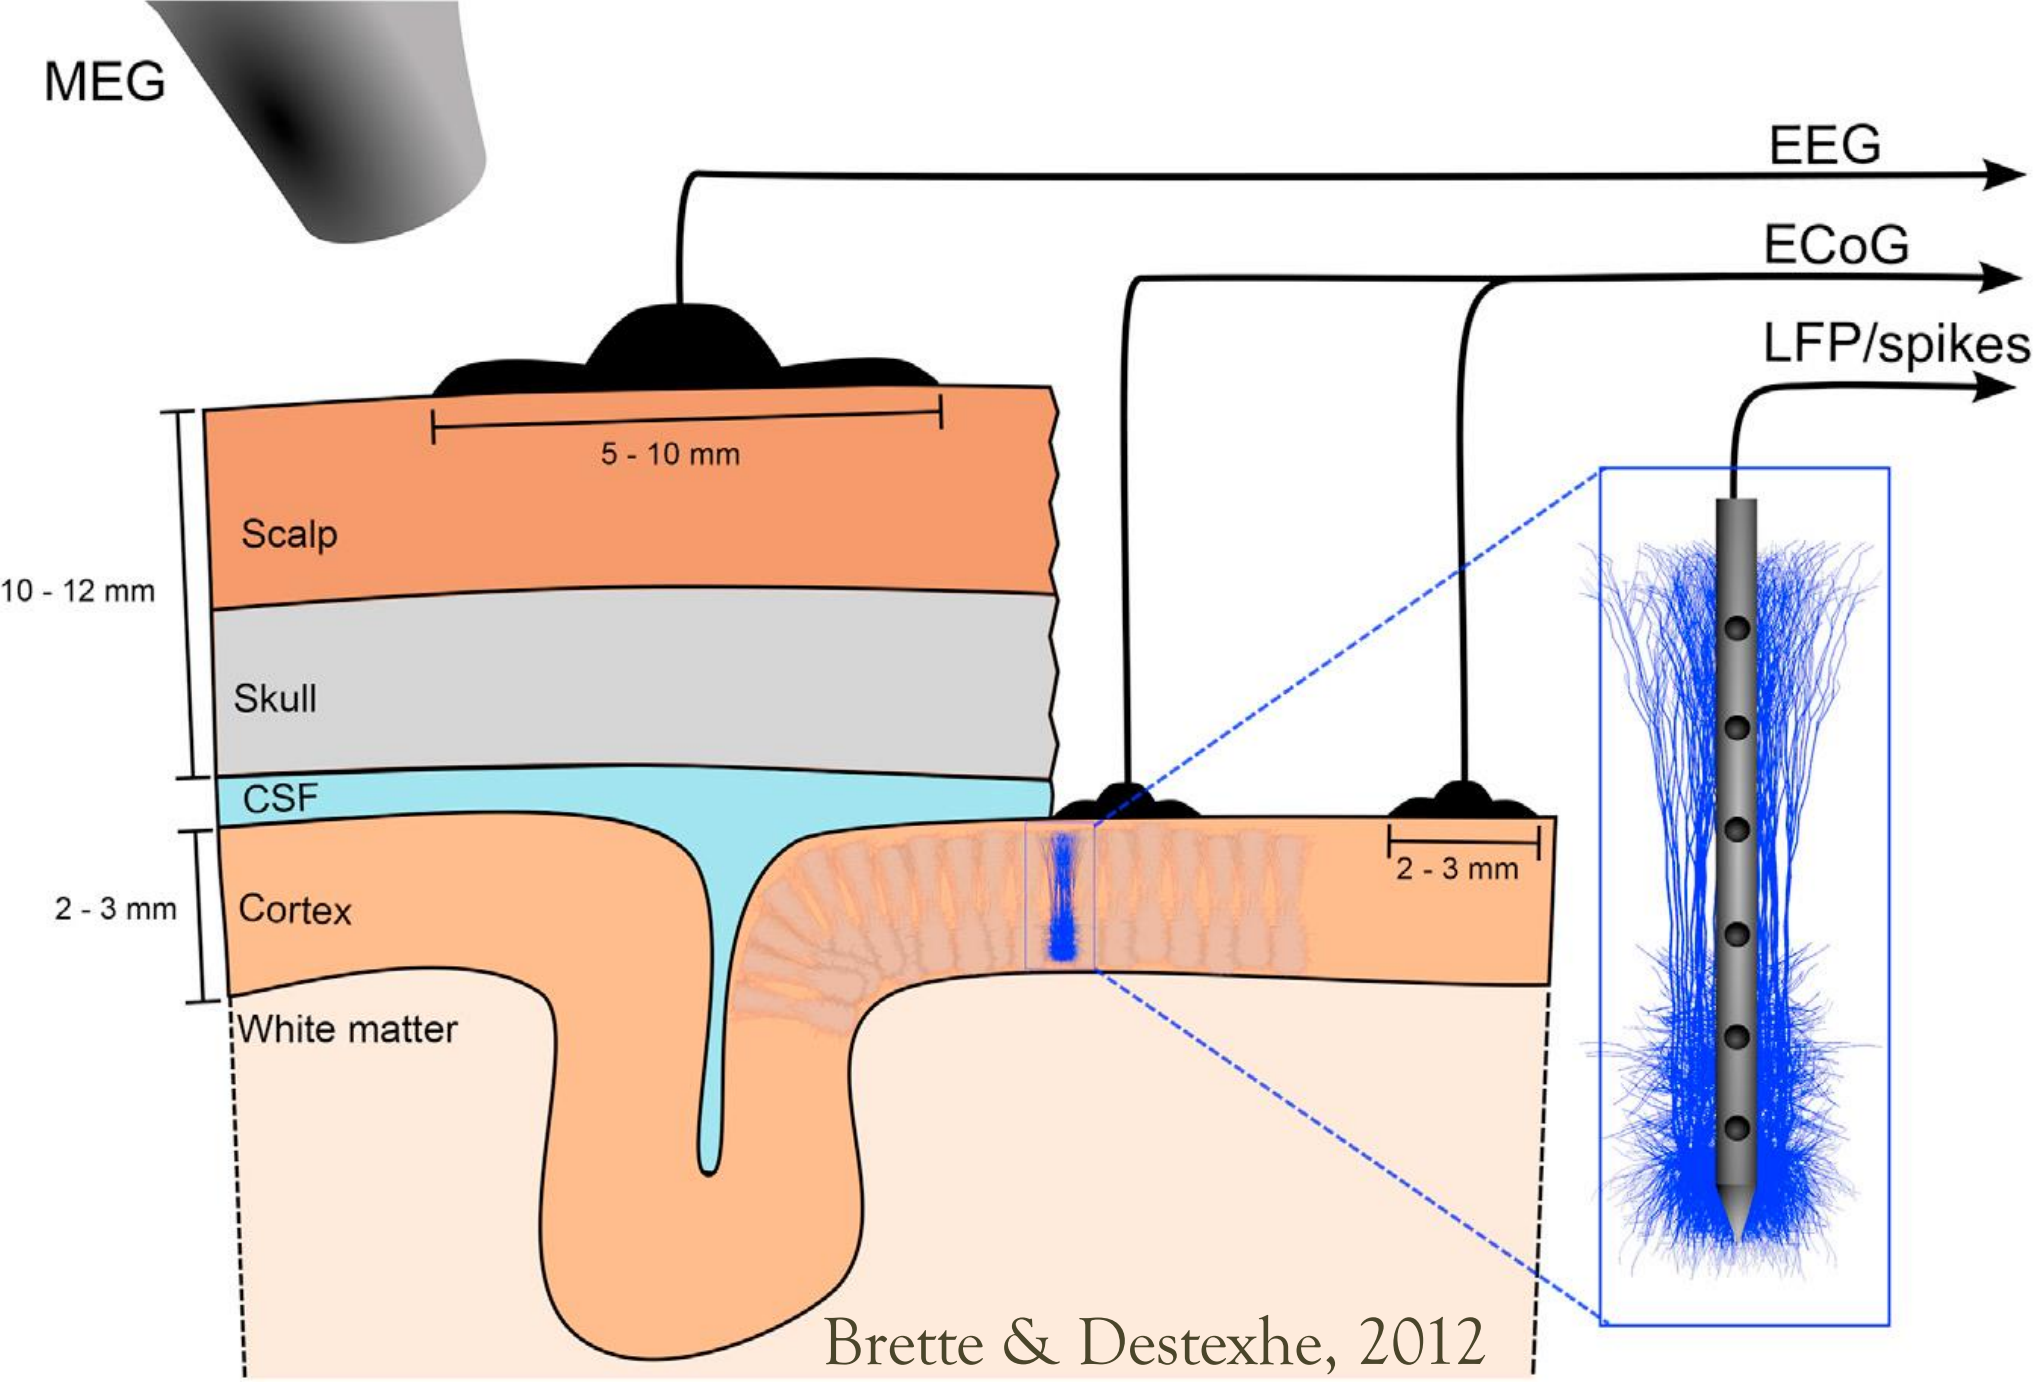
\includegraphics[scale=0.25]{01_1}
    \centering
\end{figure}
Finally, it should be stated that there is still no comprehensive theory describing information
processing in the brain, but important building blocks can be won through these approaches and
may constitute the basis for such a theory in the future.
\newpage

\section{Neuron Components and Equivalent Circuit}
\graphicspath{ {./images/02/} }
A neuron is made of several fundamental components, crucial to build a meaningful model.
\begin{itemize}
    \item \textbf{Anatomical components:}
          \begin{itemize}
              \item Soma
              \item Dendrites
              \item Axons
              \item Spines
              \item Synapses
          \end{itemize}
    \item \textbf{Biophysical components:}
          \begin{itemize}
              \item Cell membranes
              \item Ion channels (Na\({}^{+}\), Ca\({}^{2+}\), K\({}^{+}\), Cl\({}^{-}\), \dots)
              \item Receptors
              \item Transporters
          \end{itemize}
    \item \textbf{Sub-cellular components:}
          \begin{itemize}
              \item Binding proteins
              \item Calcium stores
              \item Intracellular signaling cascades
          \end{itemize}
\end{itemize}
When it comes to computational problems there are mainly two approaches nowadays.
\begin{itemize}
    \item \textit{Abstract models:} the functioning of neurons is abstracted, while their morphology
          is disregarded.
          \begin{figure}[H]
              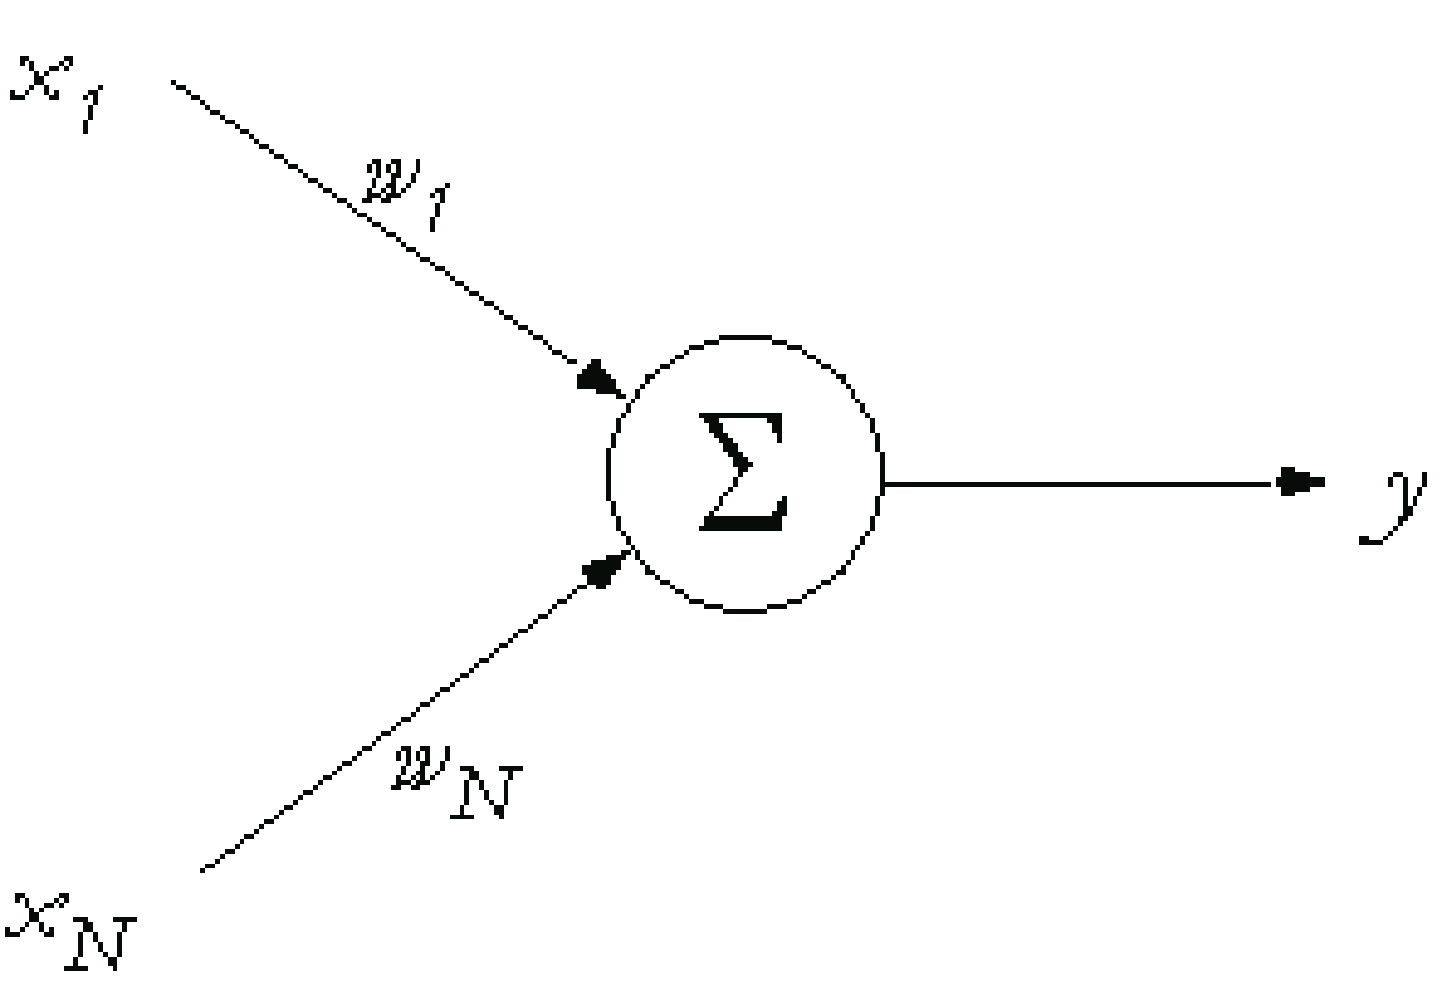
\includegraphics[scale=0.15]{02_1}
              \centering
          \end{figure}
    \item \textit{Realistic models:} the neurons morphology is kept into account as well, as it is
          considered a crucial characteristic for the model.
          \begin{figure}[H]
              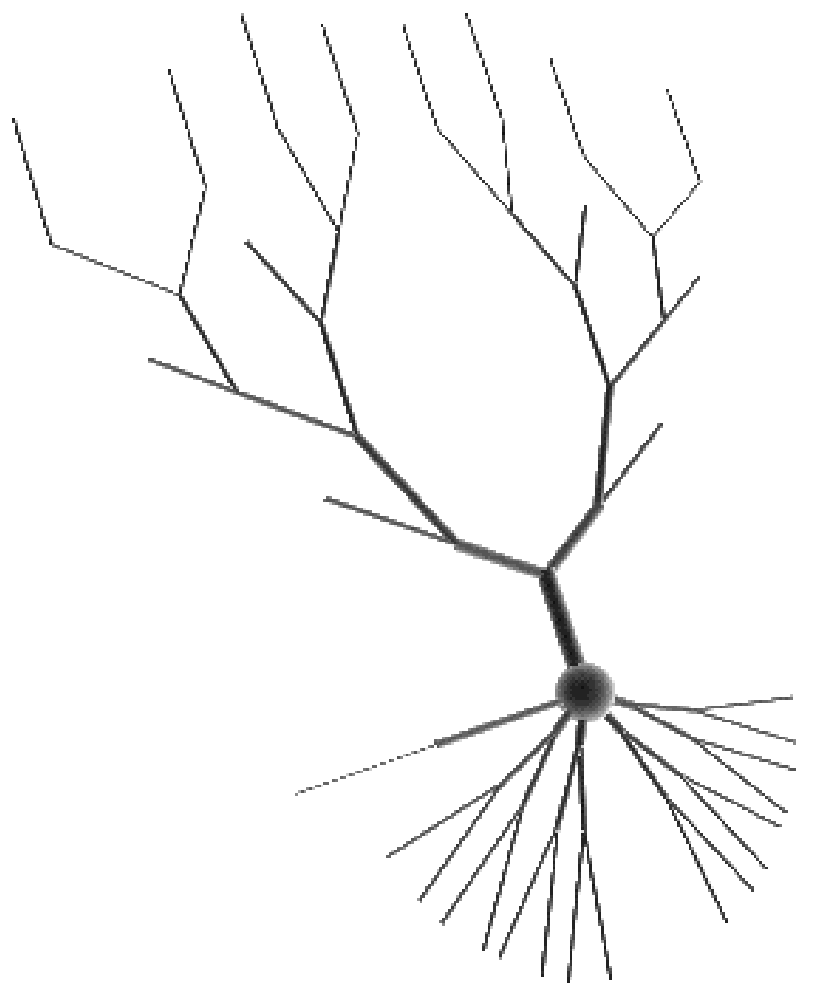
\includegraphics[scale=0.15]{02_2}
              \centering
          \end{figure}
\end{itemize}
\subsection{The Biophysical Structure of the Cell Membrane}
\paragraph{The Transmembrane Voltage}
When penetrating a neuron with a microelectrode, an electrical potential across the membrane is
measured. It is usually negative with respect to the ground (extracellular).
\begin{equation*}
    V_{m}(t)=V_{i}(t)-V_{e}(t)
\end{equation*}
The resting potential \(E_{rest}\), usually between \(-60\,mV\) and \(-70\,mV\), is the ordinary value for the
transmembrane voltage, when all the ionic currents are at the equilibrium and their net value is
zero.
\paragraph{The Transmembrane Capacitance}
A phospholipid bilayer separates the intracellular matrix from the extracellular one and it
separates ionic species, therefore it works as a capacitor, with negative charges inside the neuron
and positive charge on the outside surface:
\begin{equation*}
    Q=C_{m}\cdot V_{m}
    \hspace*{2.5cm}
    I_{C}=\frac{dQ}{dt}\Rightarrow
    I_{C}=C_{m}\frac{dV_{m}}{dt}
\end{equation*}
The membrane capacitance determines the membrane voltage dynamics, regulating how rapidly \(V_{m}\)
changes in response to a fixed current. The membrane capacitance is proportional to the surface area
of the cell, hence a specific membrane capacitance \(c_{m}\approx{1\,\mu{F}/cm^{2}}\) can be
introduced.
\paragraph{The Transmembrane Resistance}
The membrane displays voltage-independent channels with proteins allowing the leakage of ions
both into and out of the cell, iducing a current \(I_{leak}\). A leakage reversal potential
\(E_{m}\sim{E_{rest}}\) can thus be introduces. Then, the membrane voltage changes in a linear way,
following the Ohm's law:
\begin{equation*}
    V_{m}=R_{m}\cdot{I_{leak}}
\end{equation*}
where \(R_{m}\) is the transmembrane resistance. Notice that such a resistance is often
characterized by the related channel conductance \(g_{leak}=\frac{1}{R_{m}}\).\\
Holding the membrane potential steady at a level different from \(E_{rest}\) requires a certain
current, which is determined by the membrane (or input) resistance \(R_{m}\). Also in this
case it is possible to define the specific membrane resistance \(r_{m}\), independent on the
cell surface area.\\
\newline
To sum up, a neuron can be characterized by the measures reported in the picture below.
\begin{figure}[H]
    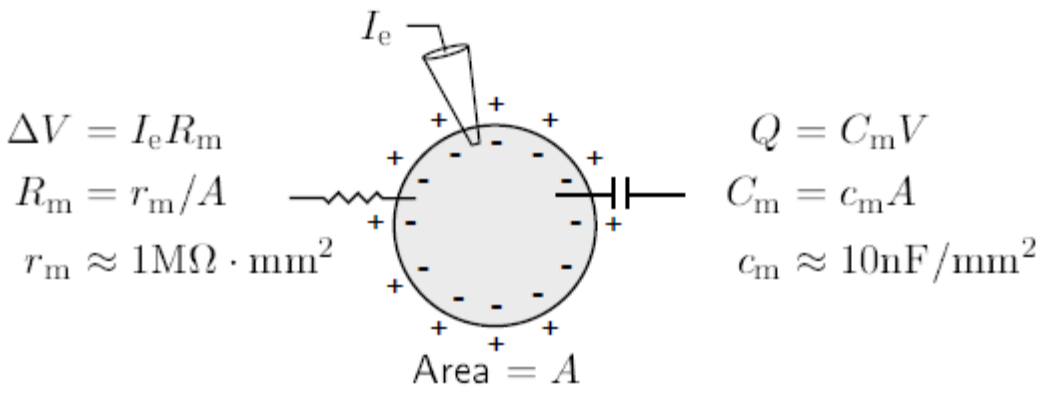
\includegraphics[scale=0.45]{02_3}
    \centering
\end{figure}
The membrane capacitance \(C_{m}\) and the membrane resistance \(R_{m}\) are employed to define
a membrane time constant \(\tau_{m}=R_{m}\cdot{C_{m}}=r_{m}\cdot{c_{m}}\) regulating the time
scale of changes in the membrane potential. It typically ranges in the \(10\,ms-100\,ms\) interval.\\
Now, the reported equivalent circuit can be derived from the previous considerations and the
relative KCL is shown just below it.
\begin{figure}[H]
    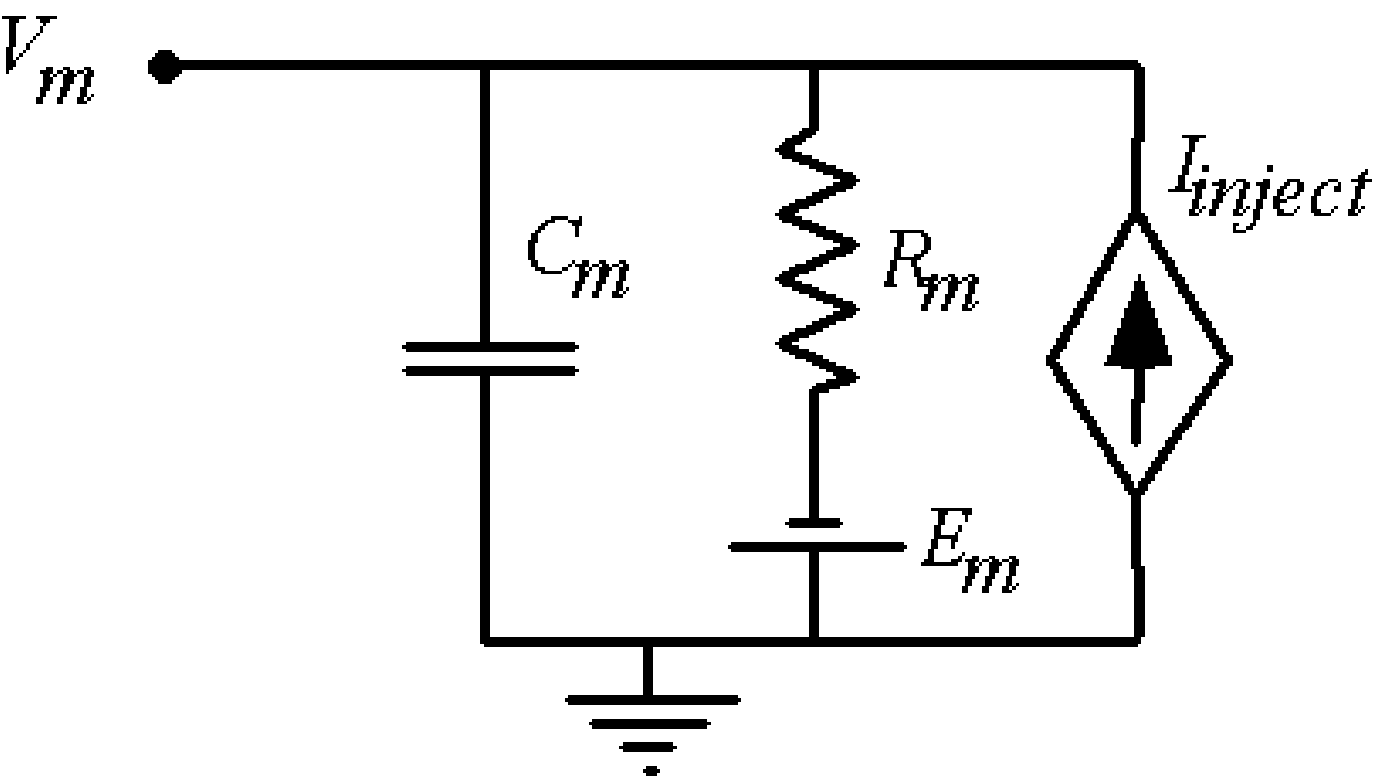
\includegraphics[scale=0.25]{02_4}
    \centering
\end{figure}
\begin{equation*}
    C_{m}\frac{dV_{m}}{dt}=-\frac{(V_{m}-E_{m})}{R_{m}}+I_{inject}
\end{equation*}
By solving the KCL, an expression for the membrane voltage as a function of time is obtained:
\begin{equation*}
    V_{m}(t)=V_{\infty}\bigl(1-e^{-\frac{t}{\tau_{m}}}\bigr)+E_{m}
\end{equation*}
\begin{equation*}
    \text{with}
    \hspace{0.25cm}
    V_{\infty}=R_{m}\cdot{I_{inject}}
    \hspace{0.25cm}
    \text{and}
    \hspace{0.25cm}
    \tau_{m}=R_{m}\cdot{C_{m}}
\end{equation*}
\subsection{Modelling the Single Channel}
So far, voltage-independent channels have been taken into account. However, cell membranes
contains a number of individual (voltage-dependent) channels. These channels open in a stochastic
way and their opening may be affected by several factors, such as the membrane potential \(V_{m}\),
intracellular ion concentration, and so on. Moreover, they are selective for one or more ions,
typically Na\({}^{+}\), K\({}^{+}\), Ca\({}^{2+}\), and Cl\({}^{-}\).
\begin{figure}[H]
    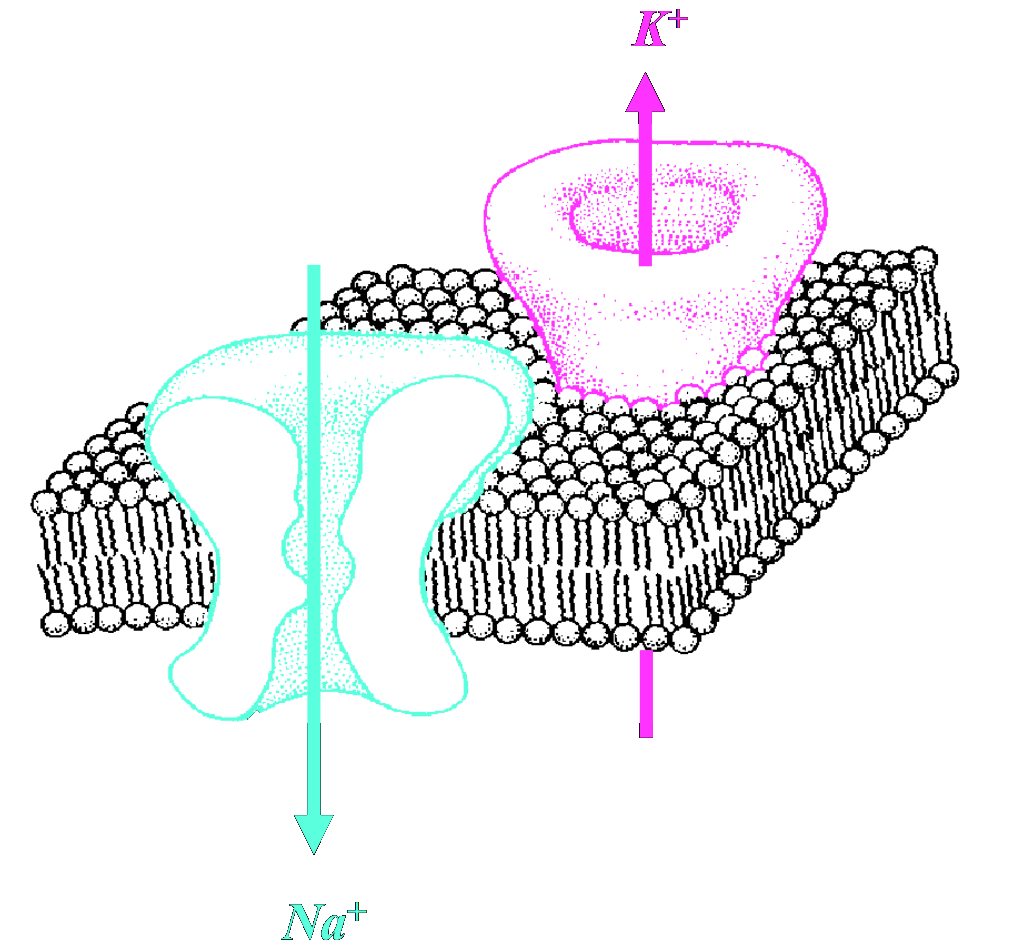
\includegraphics[scale=0.3]{02_5}
    \centering
\end{figure}
Whenever ions flow through these channels, some ionic currents \(I_{k}\) are generated. Generally,
\(I_{k}\) is related to the membrane voltage \(V_{m}\) through a linear relationship, leading
to the following equation.
\begin{equation*}
    I_{k}=g_{k}(V_{m}-E_{k})
\end{equation*}
Note that the conductance \(g_{k}\) is a function of several factors, in particular
\(g_{k}=f(V_{m},[k],t)\), with the ionic reversal potential \(E_{k}\) defined by the Nernst
equation as \(E_{k}=\frac{RT}{zF}\ln{\frac{[k]_{out}}{[k]_{in}}}\).\\
These voltage-dependent or concentration-dependent ionic currents can be incorporated in the
previously introduced equivalent circuit:
\begin{figure}[H]
    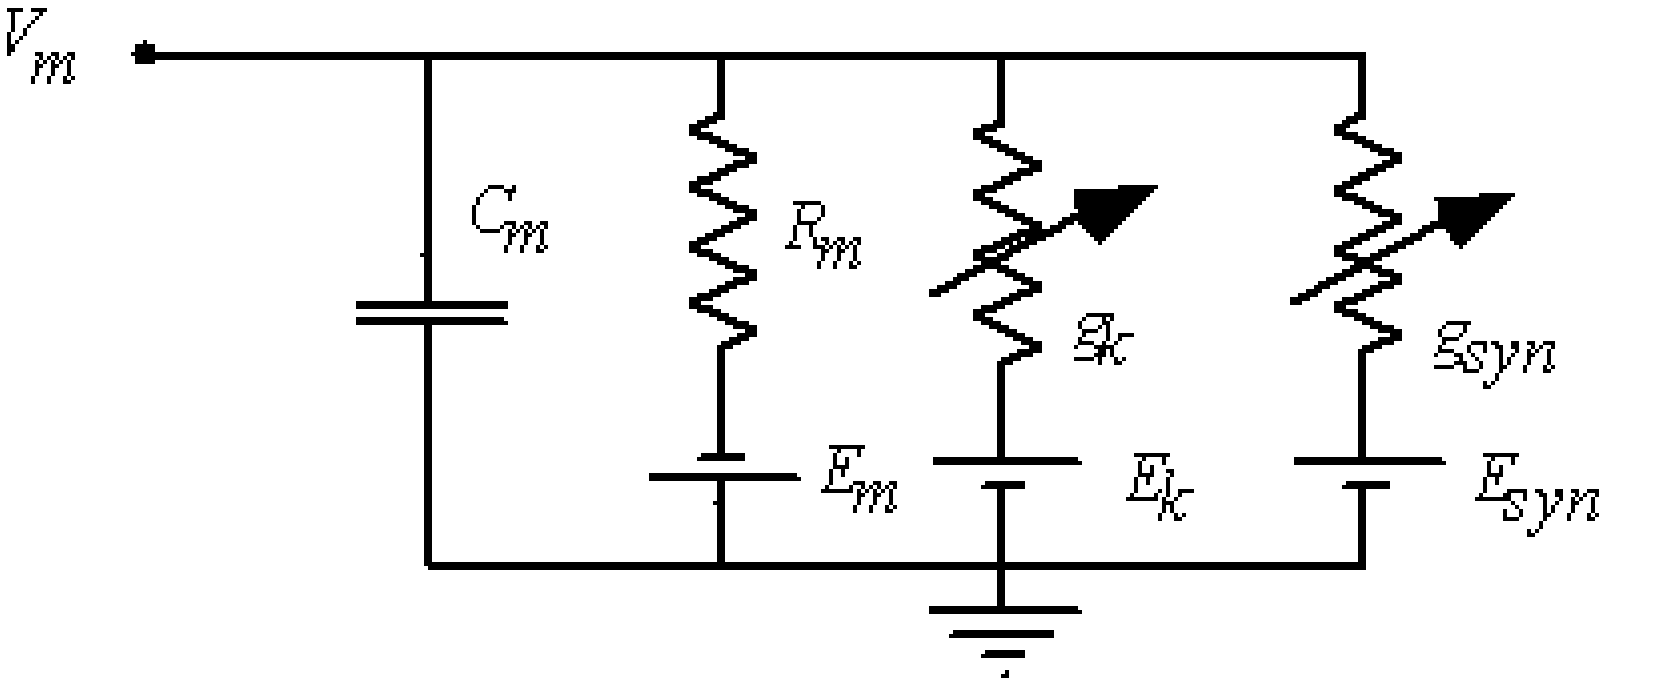
\includegraphics[scale=0.3]{02_6}
    \centering
\end{figure}
\begin{equation*}
    I_{k}=g_{k}(V_{m}-E_{k})
    \hspace{2.5cm}
    I_{syn}=g_{syn}(V_{m}-E_{syn})
\end{equation*}
Note that \(g_{syn}\) and \(E_{syn}\) are the synaptic conductance and the synaptic reversal
potential respectively.
\paragraph{Why are ionic channels modeled as resistive circuits?} The flux of ions through each
transmembrane ionic channel is ruled by both \textit{drift} and \textit{diffusion}. As a
consequence, they give birth to a drift-diffusion (ionic) current \(I_{k}\).
\begin{align*}
    I_{k}(x)
     & =I_{k,diffusion}(x)+I_{k,drift}(x)                      \\
     & =-z_{k}FD_{k}\frac{d[k](x)}{dx}+z_{k}F[k](x)\mu_{k}E(x)
\end{align*}
where \(E(x)\) is the electric field across the membrane.\\
By rearranging the equation, it can be obtained that:
\begin{equation*}
    \frac{I_{k}(x)}{\mu_{k}z_{k}F}=-\frac{D_{k}}{\mu_{k}}\frac{d[k](x)}{dx}+[k](x)E(x)
\end{equation*}
Note that due to the Einstein relationship \(\frac{D_{k}}{\mu_{k}}=\frac{RT}{z_{k}F}\), therefore:
\begin{equation*}
    \frac{I_{k}(x)}{\mu_{k}z_{k}F[k]}=
    -\frac{RT}{z_{k}F}\frac{1}{[k](x)}\frac{d[k](x)}{dx}-\frac{dV(x)}{dx}
\end{equation*}
Let's now integrate all the terms:
\begin{equation*}
    \int_{0}^{\Delta{x}}{\frac{I_{k}(x)}{\mu_{k}z_{k}F[k]}}dx=
    -\frac{RT}{z_{k}F}\int_{[k]_{in}}^{[k]_{out}}{\frac{1}{[k](x)}d[k](x)}
    -\int_{V_{in}}^{V_{out}}{dV(x)}
\end{equation*}
where \(\Delta{x}\) is the membranes thickness. At this point let's assume current density which
is constant across the membrane, such that it can be taken outside the integral.
\begin{equation*}
    I_{k}\int_{0}^{\Delta{x}}{\frac{1}{\mu_{k}z_{k}F[k]}}dx=
    -\frac{RT}{z_{k}F}\ln{\frac{[k]_{out}}{[k]_{in}}}
    -(V_{out}-V_{in})
\end{equation*}
Note that \(\int_{0}^{\Delta{x}}{\frac{1}{\mu_{k}z_{k}F[k]}}dx=R_{k}\), while
\(V_{in}-V_{out}=V_{m}\), leading to:
\begin{equation*}
    I_{k}{R_{k}}=V_{m}-E_{k}
\end{equation*}
This is the Ohm's law and this relationship has been derived without any assumption on the nature
of ionic channels or about their opening and closing dynamics.\\
Eventually, a crucial remark consists in saying that the electrophysiological properties of a
neuron are not exclusively caused by peculiar kinds of channels across its membrane. Also the
neuron morphology plays a fundamental role, thus it has to be modeled too.
\newpage

\section{Modeling Complex Neuronal Structures}
\graphicspath{ {./images/03/} }
When dealing with neurons, it must be kept in mind that there are several types of
neurons characterized by peculiar morphologies and arborizations, fundamental
to properly build an effective and reliable model.\\
To encode the structure of a neuron it is necessary to acquire images of the cell itself:
this is often done via radioactive or fluorescent markers, alternatively advanced optical
methods are often employed. Successively, the model has to be quantitatively characterized,
thus the dimensions of each cell element are measured.\\
Several softwares, such as \textit{NeuroMorpho}, were introduced to reconstruct 3D models of
neurons, allowing scientists to share them across the scientific community.

\subsection{Compartmental Models}
Generally, the morphology of the dendritic arborizations is the main attribute used to classify
neurons. Compartmental models are based on the idea that the various structures found in
a neuron can be modelled separately, then they are put together, constituting the
overall realistic and working model of the target cell.\\
In order to compartmentalize a neuron, the structure is divided into three main parts:
\begin{itemize}
    \item \textbf{Soma}: it is commonly approximated to a isopotential spheroid. the
          transition points between the soma and the dendritic tree are difficult to determine.
    \item \textbf{Dendritic Tree}: it is often modelled as a complex structure made by
          linked sequences of discrete cylinders, characterized by geometrical properties.
    \item  \textbf{Dendritic Spines}: they are the major target of synapses, making their
          modelling rather complex.
\end{itemize}
During the development of a model, it is crucial to keep in mind the following relatonships:
\begin{equation*}
    {Model\,fidelity}\propto{Amount\,of\,data}
    \hspace{2.5cm}
    {Simulation\,speed}\propto{\frac{1}{Model\,fidelity}}
\end{equation*}
An example of compartmental model is reported below, in particular the KCL and KVL for the
\(j-\)th element are shown:
\begin{figure}[H]
    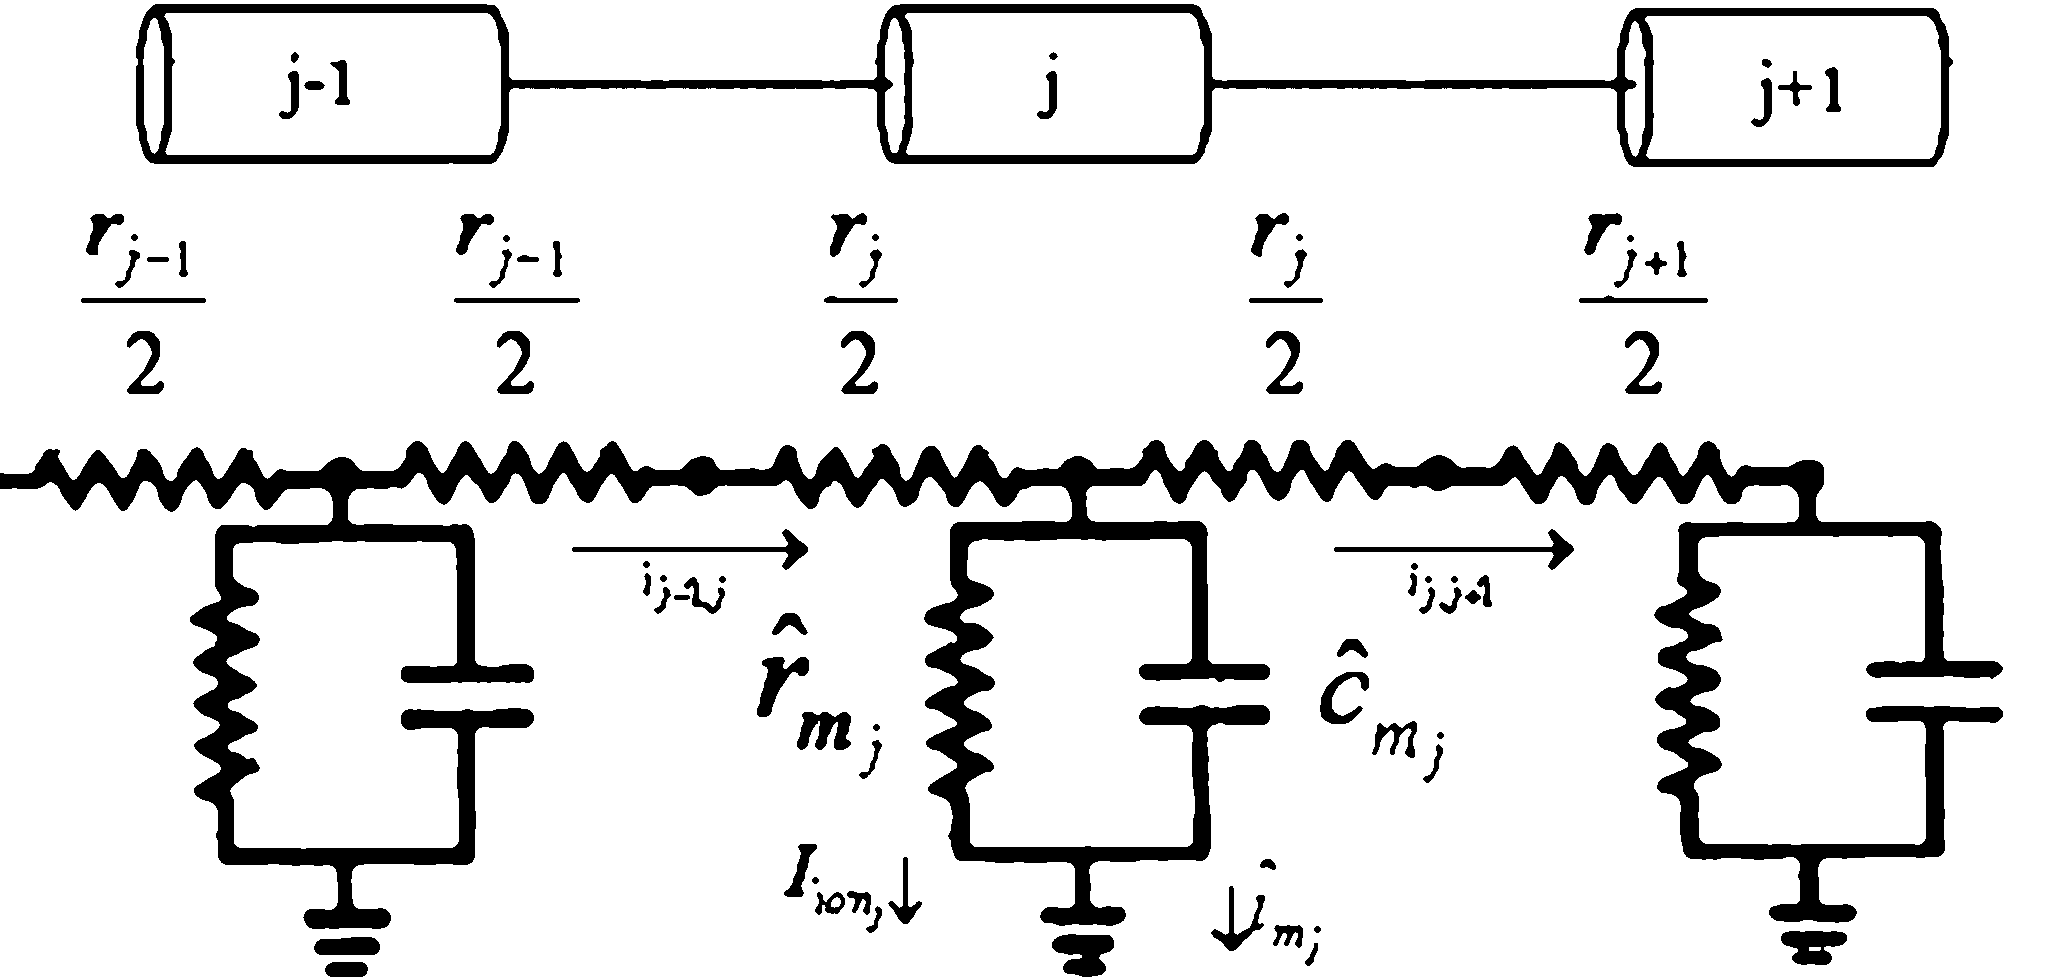
\includegraphics[scale=0.17]{03_1}
    \centering
\end{figure}
\begin{equation*}
    \begin{cases}
        \hat{i}_{m_{j}}=\hat{i}_{m_{j-1,j}}-\hat{i}_{m_{j}}=\hat{i}_{m_{j,j+1}} \\
        \hat{i}_{m_{j}}=I_{ion,j}+\hat{c}_{m}\frac{dV_{j}}{dt}+I_{stim,j}       \\
        \hat{i}_{m_{j}}=\frac{V_{j-1}-V_{j}}{r_{j-1,j}}-\frac{V_{j}-V{j+1}}{r_{j,j+1}}
    \end{cases}
    \Rightarrow
    \hat{c}_{m}\frac{dV_{j}}{dt}+I_{ion,j}+I_{stim,j}=g_{j-1,j}(V_{j-1}-V_{j})-g_{j,j+1}(V_{j}-V_{j+1})
\end{equation*}
In the equations above, \(r_{j}\) denotes the (specific) axoplasmatic resistance and \(I_{ion,j}\)
the ionic currents, including leakage and active channels, as well as synaptic contributions.
The main questions that should be answered when building a compartmental model regard the
compartmentalization criterion to employ, the estimation of the dendrites diameter if it is
not constant, and whether and how to take into account the dendritic spines. Therefore,
a segmentation (or compartmentalization) method is required.
\begin{figure}[H]
    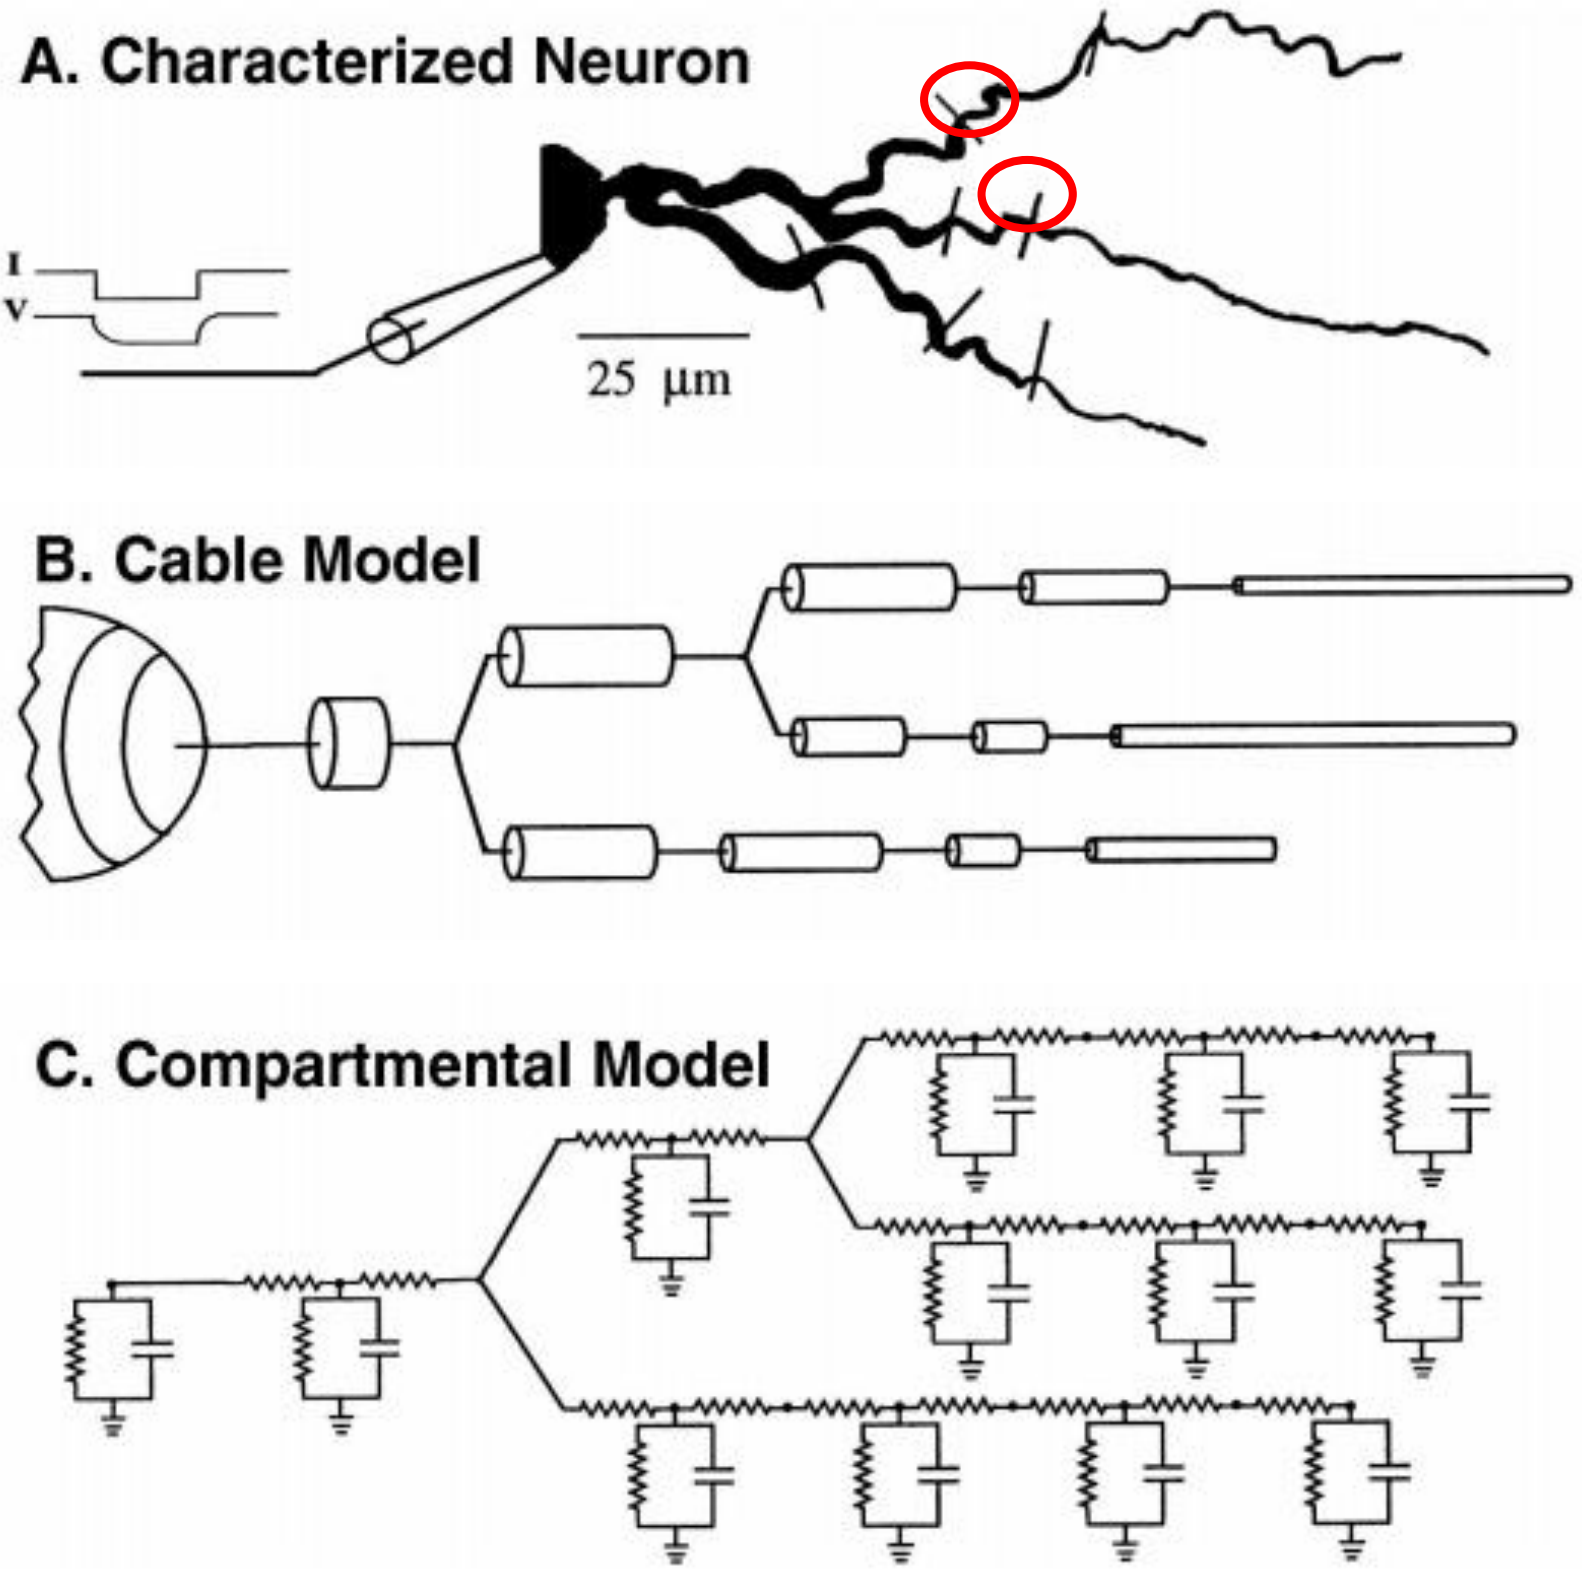
\includegraphics[scale=0.25]{03_2}
    \centering
\end{figure}
After characterizing the neuron from a geometrical point of view, a cable model, where
each dendritic segments is approximated to a cable with a specific diameter, is constructed.
Note that a threshold on the diameter is usually exploited, in order to have a discrete
set of diameters. Finally, each cable segment is considered to be isopotential and is modelled
through an equivalent electrical circuit.

\subsection{Complexity Reduction}
Given their nature, realistic and detailed compartmental models tend to be particularly
demanding from the computational point of view. Hence, the main idea is to simplify them,
losing some details in order to increase their efficiency. To do so, their level of
abstraction is increased.
\begin{figure}[H]
    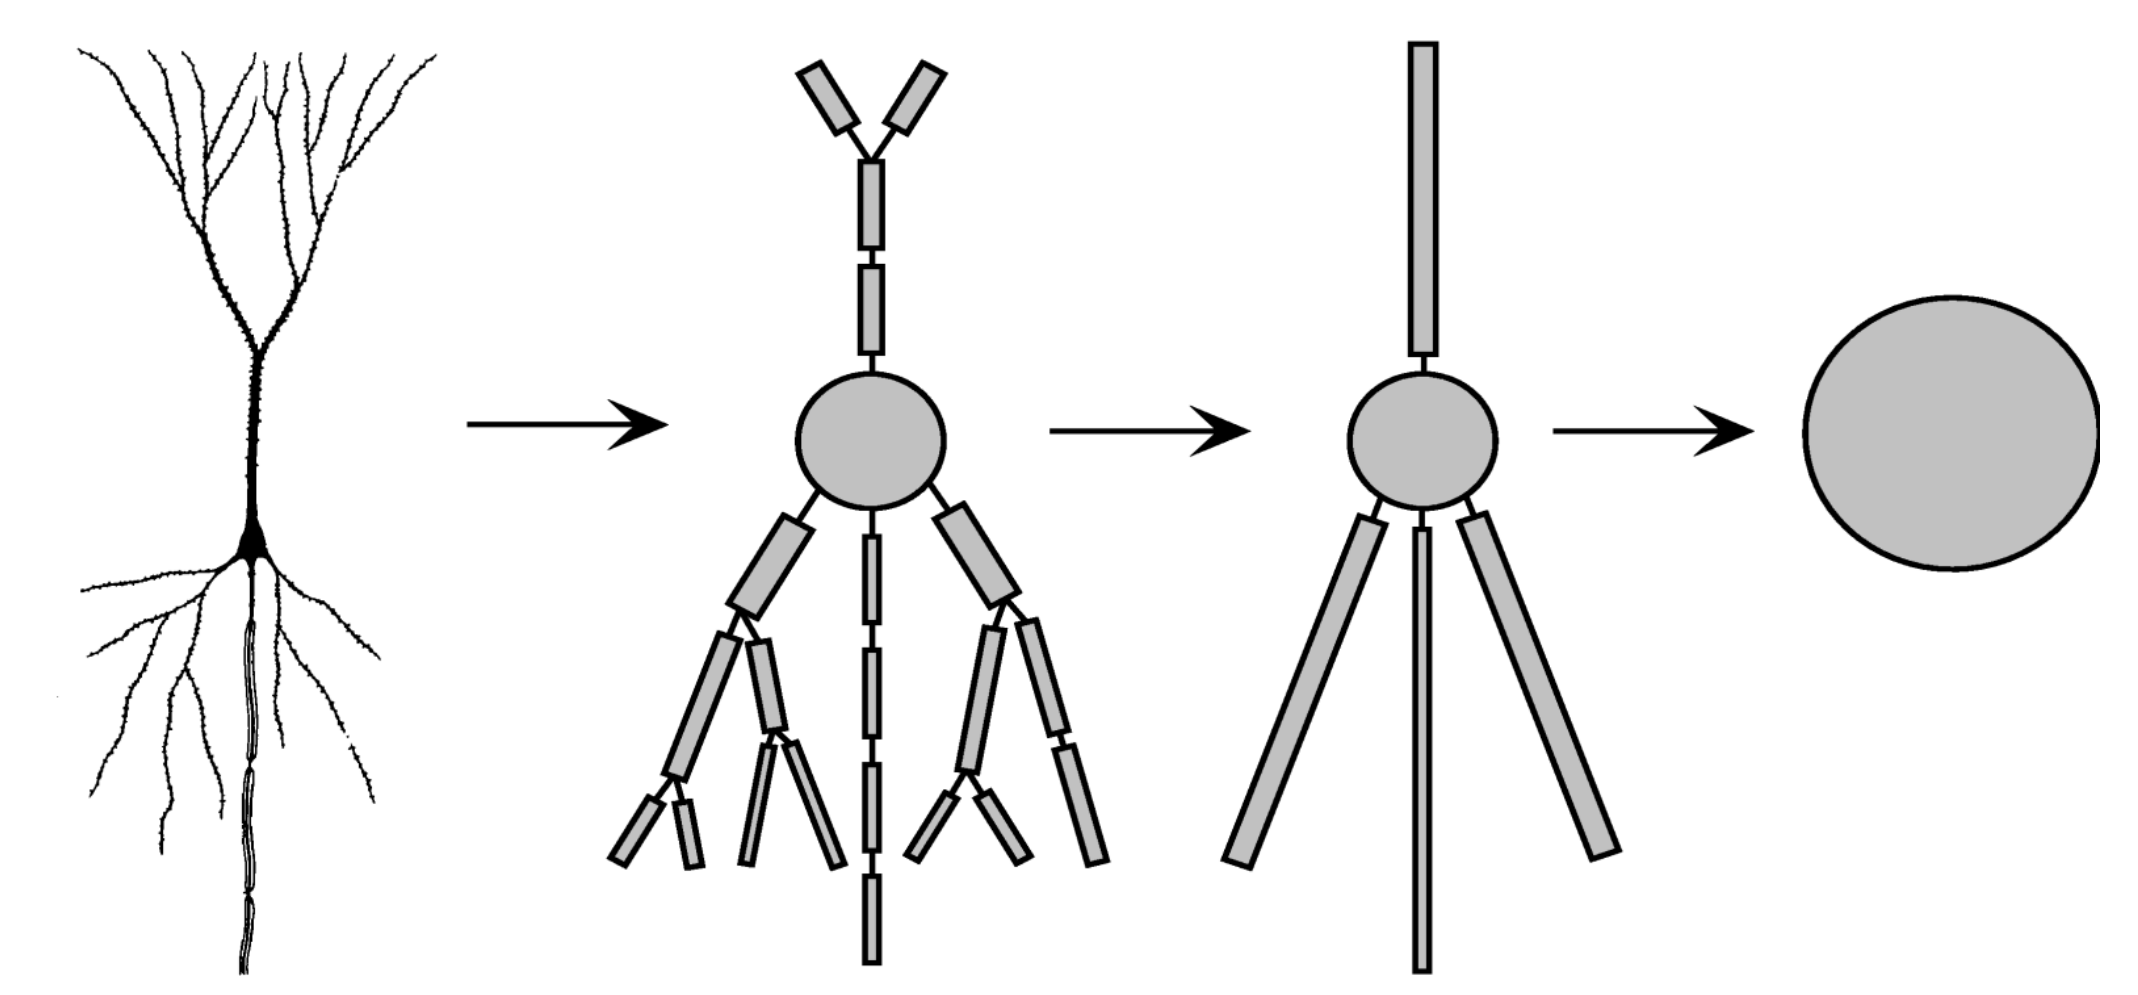
\includegraphics[scale=0.2]{03_3}
    \centering
\end{figure}
The aim is to reduce complexity while keeping the very same electrophysiological patterns,
such as bursts, spikes, and mixed activity. On the other hand, reducing a model inevitably
leads to losing certain features, ISI for instance, but it is not important as long as
these attributes are not relevant to characterize the considered model. The golden rule
when simplifying a neuronal model is that the input/output characteristic, which is
derived from stimulations, should not change. Note that the neuron spontaneous activity is
instead strictly related to the cell morphology, thus it is extremely difficult to
preserve it during model reduction.
\begin{figure}[H]
    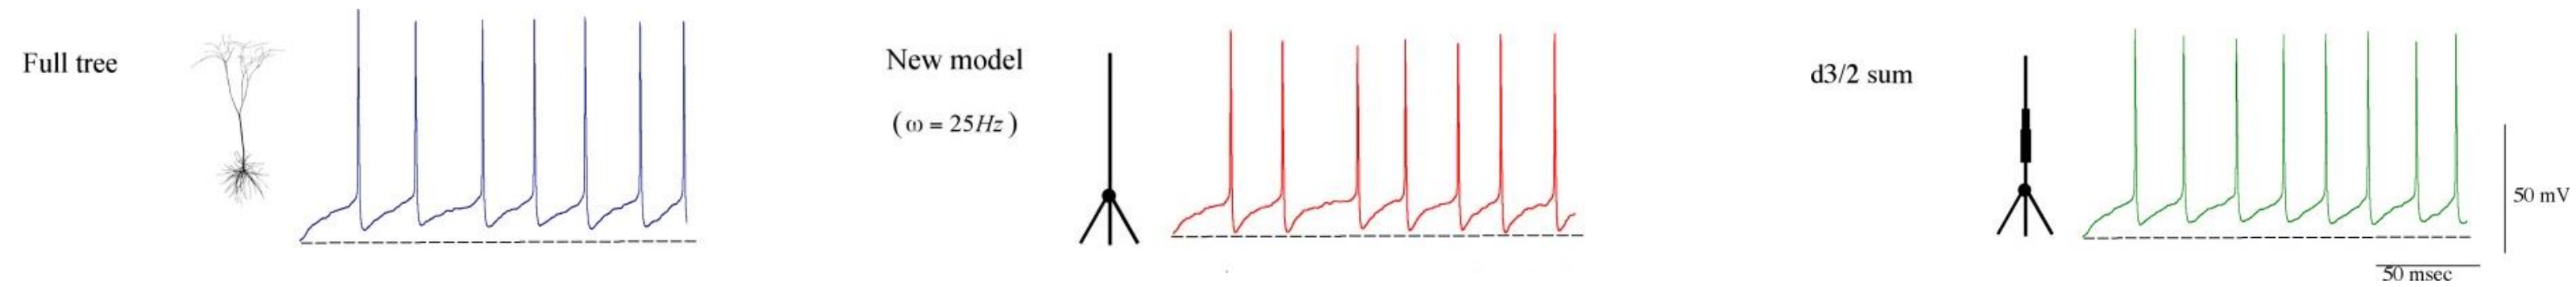
\includegraphics[scale=0.25]{03_4}
    \centering
\end{figure}
\paragraph{The Rall's Equivalent Cylinder}
The main idea is that the whole dendritic tree of a neuron can be represented as a single cylinder
having a constant diameter. In the model proposed by Rall, the soma is substituted by
a compact region (a single compartment), while the entire dendritic tree is replaced by
a single equivalent cylindrical cable. Said so, it is crucial to properly select the
geometrical and electrical properties of such a cylinder, such as its radius \(a\) and
length \(L\).
\begin{figure}[H]
    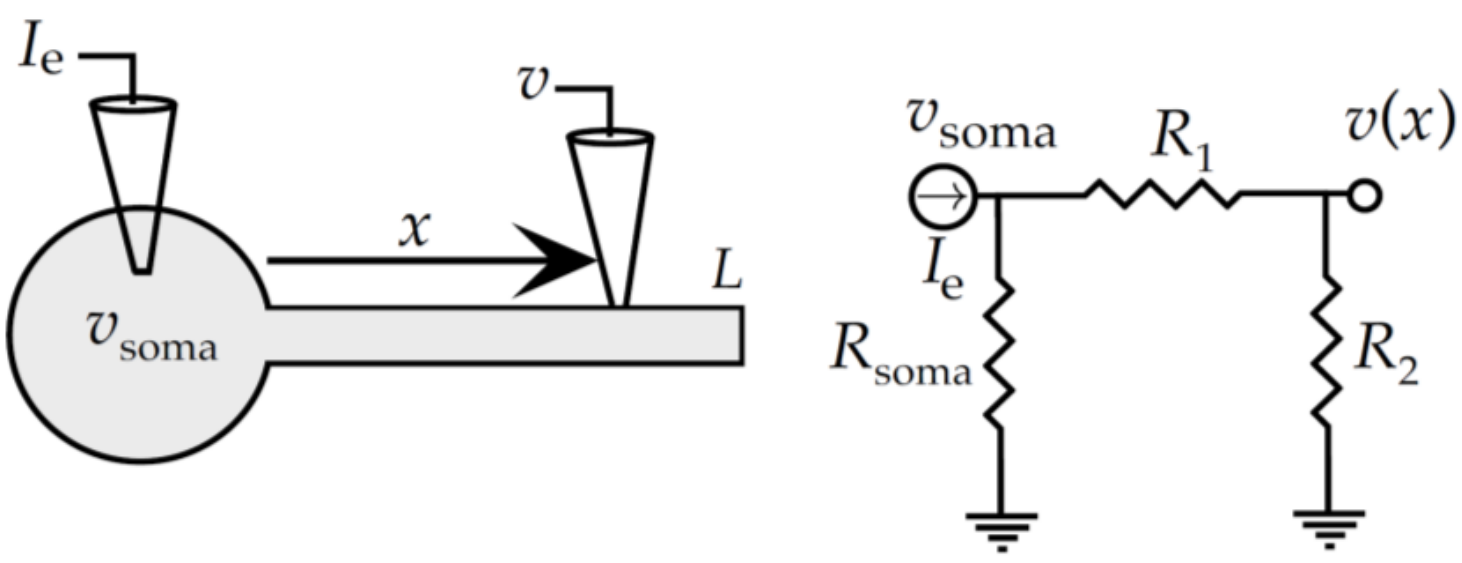
\includegraphics[scale=0.35]{03_5}
    \centering
\end{figure}
\(L\) and \(a\) are carefully selected to match two critical properties of the dendritic
tree. As a matter of fact, \(L\) is related to the average electrotonic length,
determining the degree of attenuation of the electrical input as a function of the distance.
The electrotonic length is measured by summing all the electrotonic segment lengths according
to the designated end point and then computing an average measure, describing the average
signal decay rate between the input and the output ends.\\
Differently, \(a\) is employed in the computation of the total surface area \(2\pi{a}\cdot{L}\),
crucial to correctly model the membrane resistance and capacitance of the neuron. The Rall's
model neuron input resistance \(R_{in}\) can be derived as follow:
\begin{equation*}
    R_{in}=\frac{(R_{1}+R_{2})R_{soma}}{(R_{1}+R_{2}+R_{soma})}
\end{equation*}
\begin{figure}[H]
    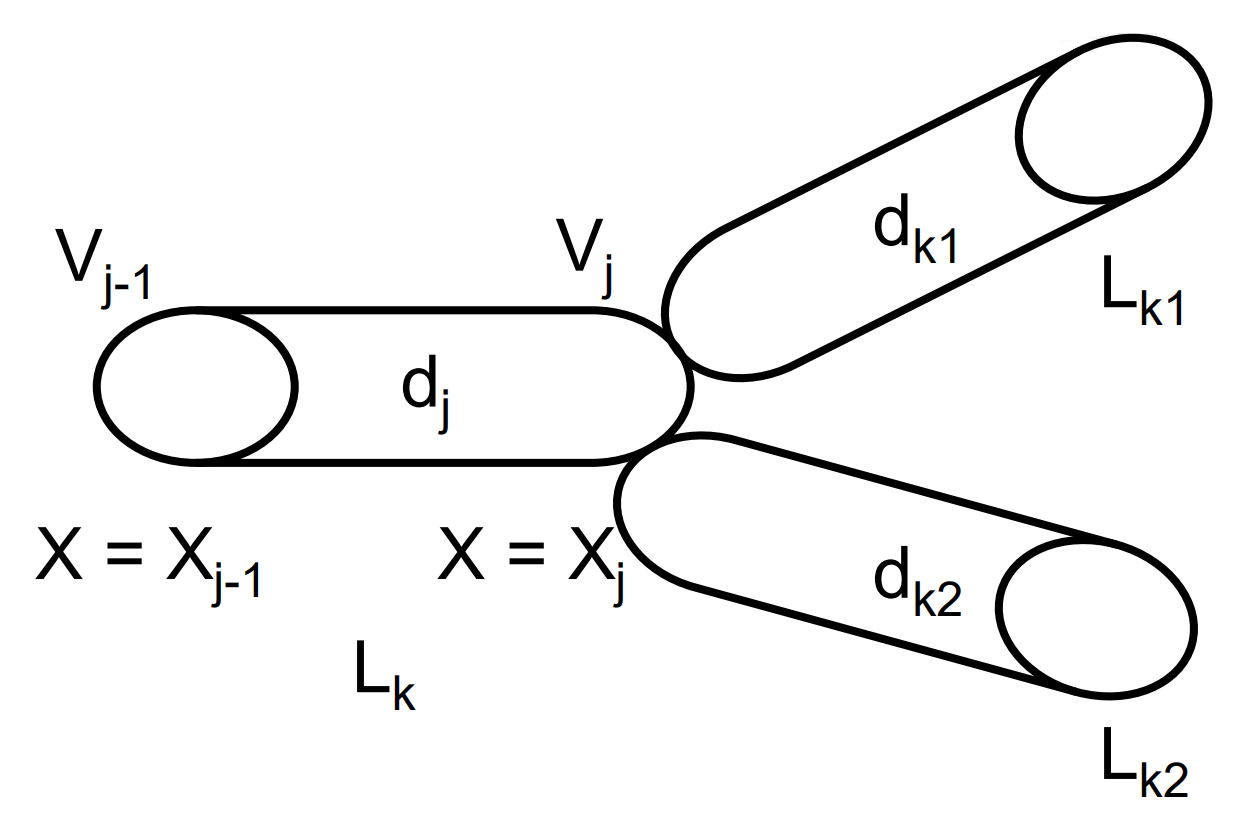
\includegraphics[scale=0.2]{03_6}
    \centering
\end{figure}
The Rall's model can be used with neurons matching three particularly strict criteria:
\begin{enumerate}
    \item The electrotonic lengths of all paths from soma to dendritic ends must be identical.
          \begin{equation*}
              L_{k}=L_{k1}=L_{k2}
          \end{equation*}
    \item The sum of the diameters of child branches at each branch point, raised to the power
          of \(\frac{3}{2}\) must equal the diameter of the parent branch, also raised to the power
          of \(\frac{3}{2}\).
          \begin{equation*}
              (d_{j})^{\frac{3}{2}}=(d_{k1})^{\frac{3}{2}}+(d_{k2})^{\frac{3}{2}}
          \end{equation*}
    \item The electrical properties should be constant and uniform as much as possible, in
          particular \(R_{m}\) and \(R_{i}\) must be spatially uniform within the branching structure.
          \begin{figure}[H]
              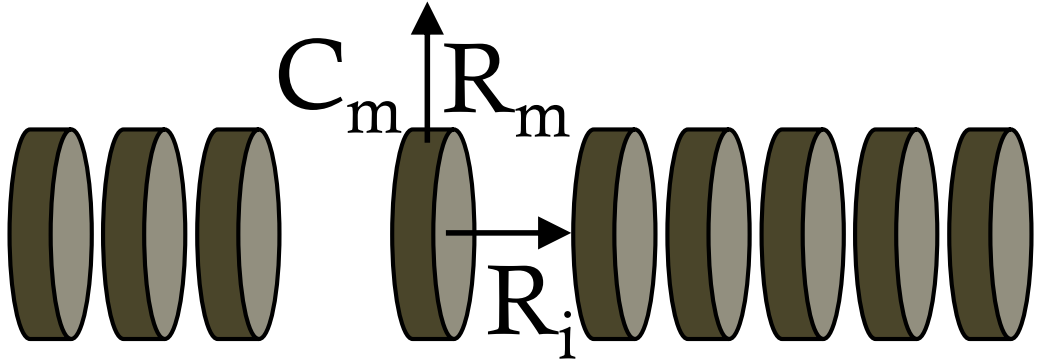
\includegraphics[scale=0.15]{03_7}
              \centering
          \end{figure}
\end{enumerate}
To sum up, the Rall's cable approach wants to substitute the whole dendritic tree with a single
cable having a constant diameter and the surface area distributed, with respect to the electrotonic
distance, similarly to the one of the original tree. Unfortunately, real neurons does not exhibit
morphological characteristics compliant with the Rall's criteria, therefore a less strict model
is to be introduced.
\paragraph{The Equivalent Cable}
This model was introduced to overcome the limitations of the Rall's cylinder, as a matter of
facts the idea is once again to model the whole dendritic tree as a single cable, but
the diameter is no longer assumed constant: it changes as a function of distance. This allows
a modelling much more precise in terms of electrical quantities, since they are strictly
related to the radius of the equivalent cable. A parameter \(\Delta{x}\) regulates the degree
of detail of the model, in particular it represents the length of a segment with constant
diameter of the overall cable. A very small \(\Delta{x}\) generates an extremely precise model,
but the computational cost increases as a consequence of the greater number of compartments.
\begin{figure}[H]
    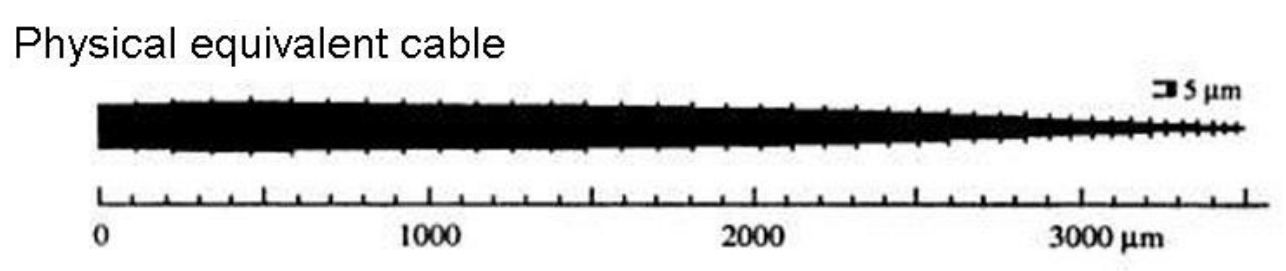
\includegraphics[scale=0.35]{03_8}
    \centering
\end{figure}
\paragraph{The Attenuation Cable}
The idea behind this approach is to disregard all the dendritic branches along which the
input signal attenuation overcomes a certain threshold: the assumption is that branches
exhibiting very fast decays are not important for the overall signal propagation.
\begin{figure}[H]
    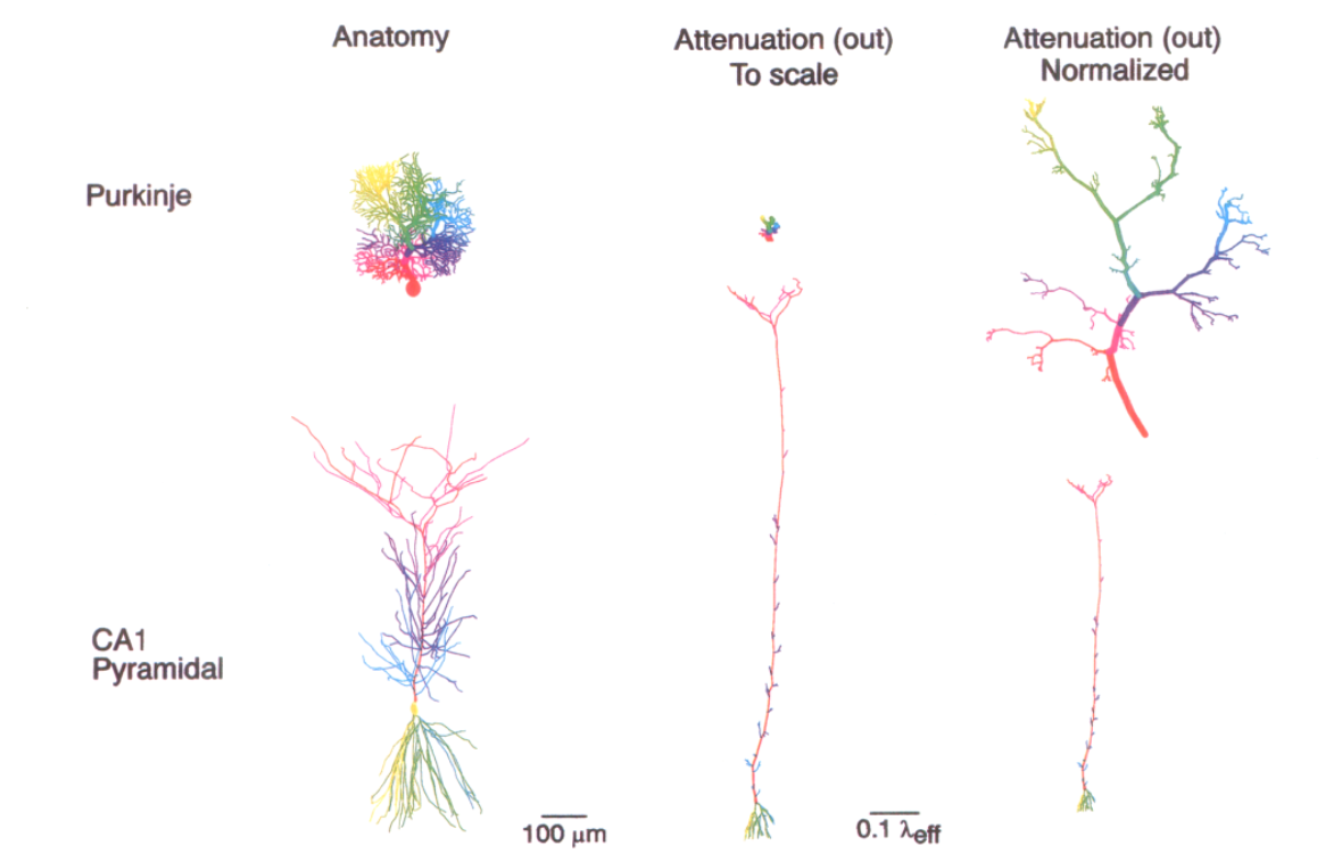
\includegraphics[scale=0.6]{03_9}
    \centering
\end{figure}
Note that the voltage attenuation is not an appropriate quantity to represent geometrically,
as it is not additive. To obtain the attenuation and delay of the membrane potential
for complex morphologies it is better to proceed as illustrated below.
\begin{figure}[H]
    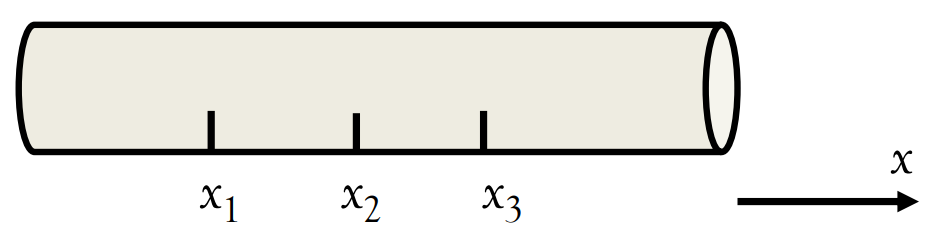
\includegraphics[scale=0.3]{03_10}
    \centering
\end{figure}
The voltage attenuation between \(x_{1}\) and \(x_{3}\) is:
\begin{equation*}
    \frac{V(x_{1})}{V(x_{3})}=\frac{V(x_{1})}{V(x_{2})}\cdot{\frac{V(x_{2})}{V(x_{3})}}
\end{equation*}
By applying the logarithm, an additive quantity is obtained, providing better information
about the signal propagation.
\begin{equation*}
    \ln{\biggl(\frac{V(x_{1})}{V(x_{3})}\biggr)}=
    \ln{\biggl(\frac{V(x_{1})}{V(x_{2})}\biggr)}+\ln{\biggl(\frac{V(x_{2})}{V(x_{3})}\biggr)}
\end{equation*}
Note that a similar approach considering signal propagation delay instead of signal
attenuation also exists.
\paragraph{The Pinsky-Rinzel 2-Comp Model}
This model is based on the fact that at least two compartments are required to properly mimic
complex patterns of electrophysiological activity. In particular, a compartment models the soma,
while another approximates the dendrites.
\begin{figure}[H]
    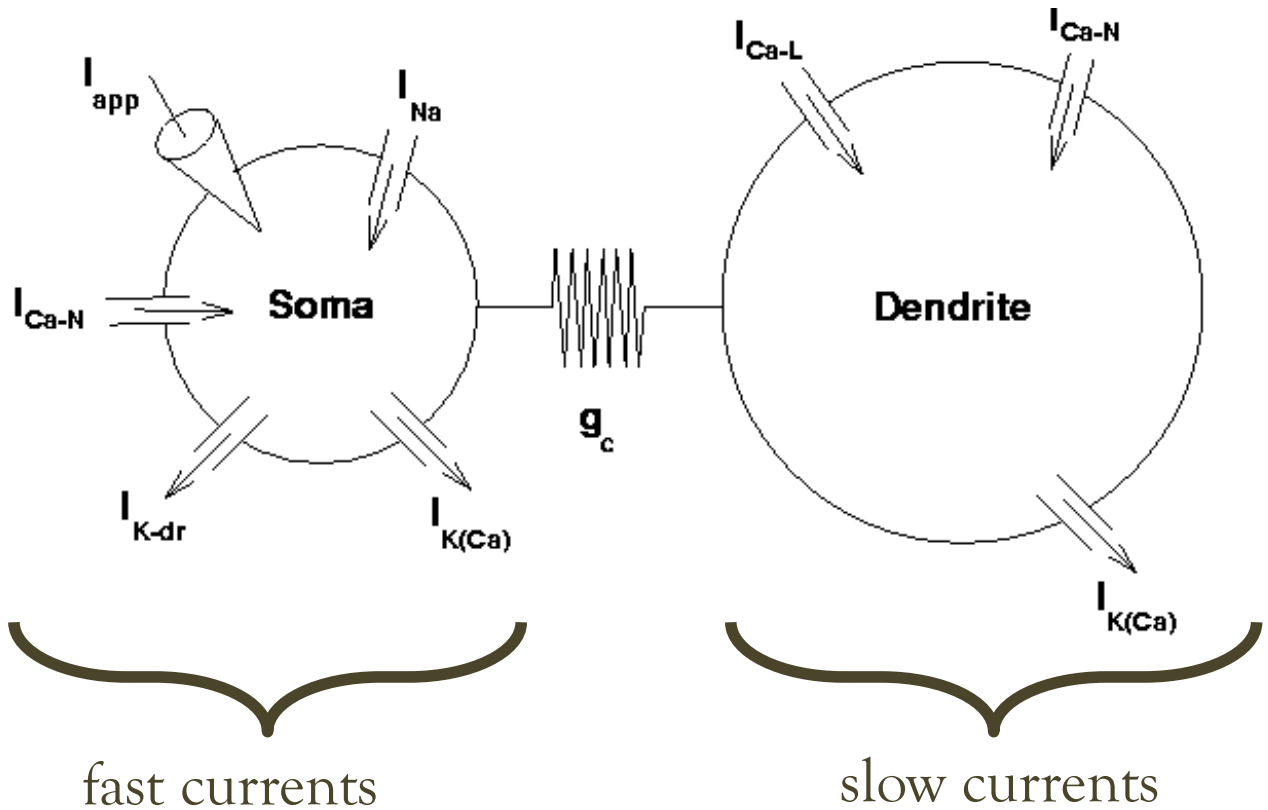
\includegraphics[scale=0.3]{03_11}
    \centering
\end{figure}
These two compartments are separated by a conductance \(g_{c}\) determining the coupling between
them, which instead regulates the kind of electrophysiological activity.
\begin{figure}[H]
    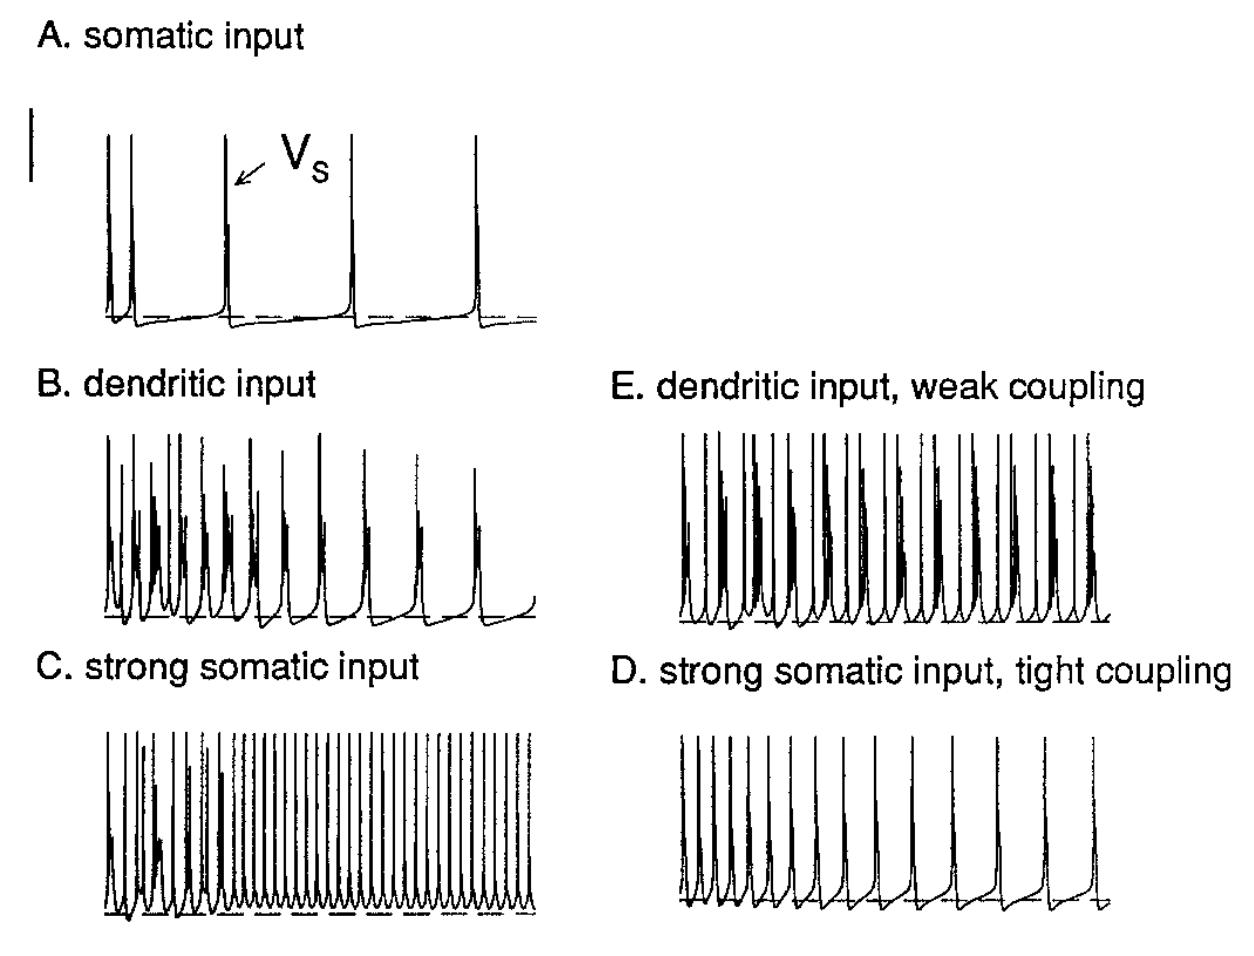
\includegraphics[scale=0.3]{03_12}
    \centering
\end{figure}

\subsection{Modelling Dendritic Spines and Synaptic Inputs}
Spines should definitely be taken into account when building the model of a neuron, they
characterize the surface of dendrites, moreover spines usually contain synapses.
\begin{figure}[H]
    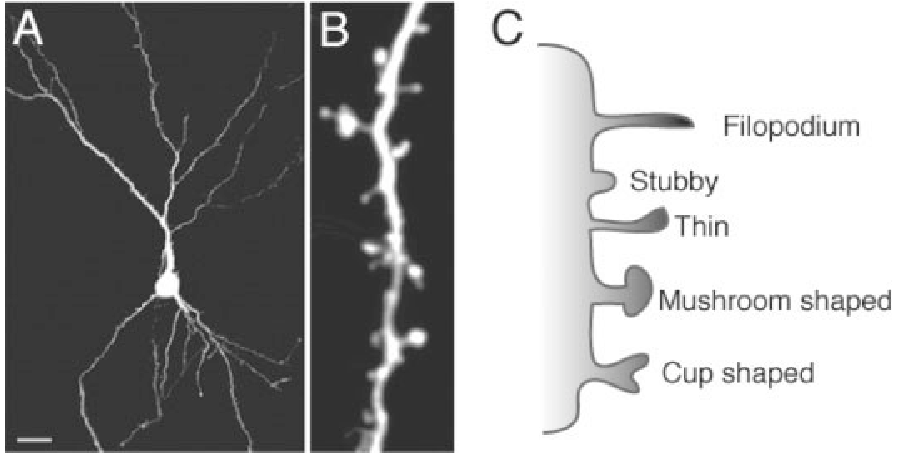
\includegraphics[scale=0.5]{03_13}
    \centering
\end{figure}
Note that several shapes are available when talking about spines, with different
geometrical properties and, as a consequence, different electrical properties.\\
When modelling spines, two distinct cases should be taken into account:
\begin{itemize}
    \item \textbf{Sipnes as \textit{passive} components}: the current flows \textit{from}
          the dendrite \textit{into} the spines.\\
          This means that spines are considered to be without synapses (no inputs). They are
          isopotential and the membrane area can be incorporated into the membrane of the parent dendrite.
          \begin{figure}[H]
              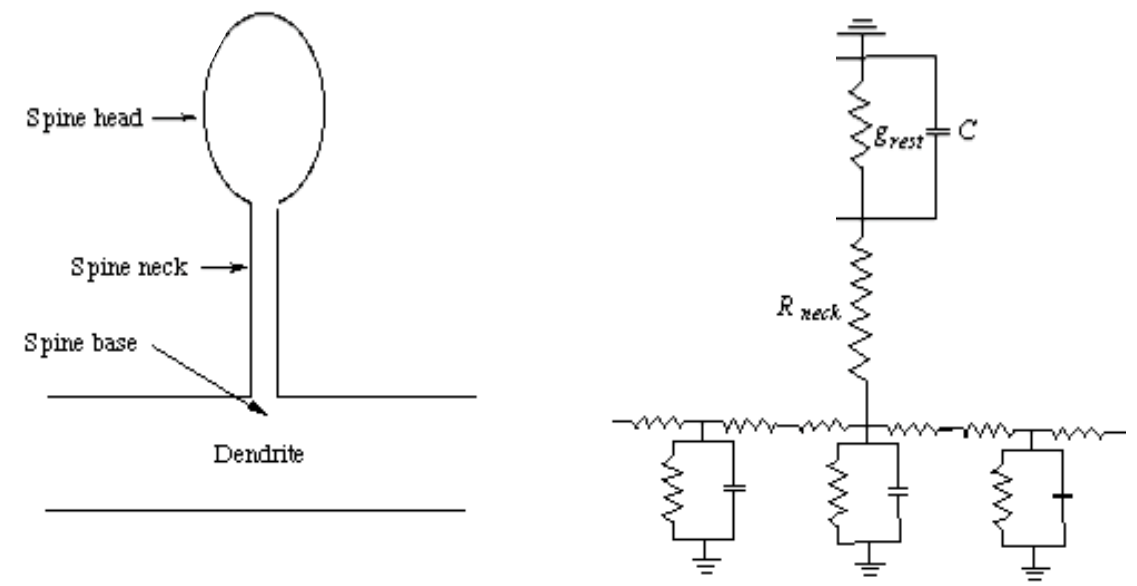
\includegraphics[scale=0.4]{03_14}
              \centering
          \end{figure}
          Both the physical dimensions and the specific membrane properties are affected by the presence
          of the spine:
          \begin{equation*}
              l'=l\cdot{F^{\frac{2}{3}}}
              \hspace{2.5cm}
              R_{m}'=\frac{R_{m}}{F}
          \end{equation*}
          \begin{equation*}
              d'=d\cdot{F^{\frac{2}{3}}}
              \hspace{2.5cm}
              C_{m}'=\frac{C_{m}}{F}
          \end{equation*}
          \begin{equation*}
              F=\frac{A_{dendrite}+A_{spine}}{A_{dendrite}}
          \end{equation*}
    \item \textbf{Sipnes as \textit{active} components}: the current is generated at the head membrane.\\
          In this case the spine contains a synapse, as an input current flows into it. The synaptic input
          can be modelled through a time-varying synaptic conductance.
          \begin{figure}[H]
              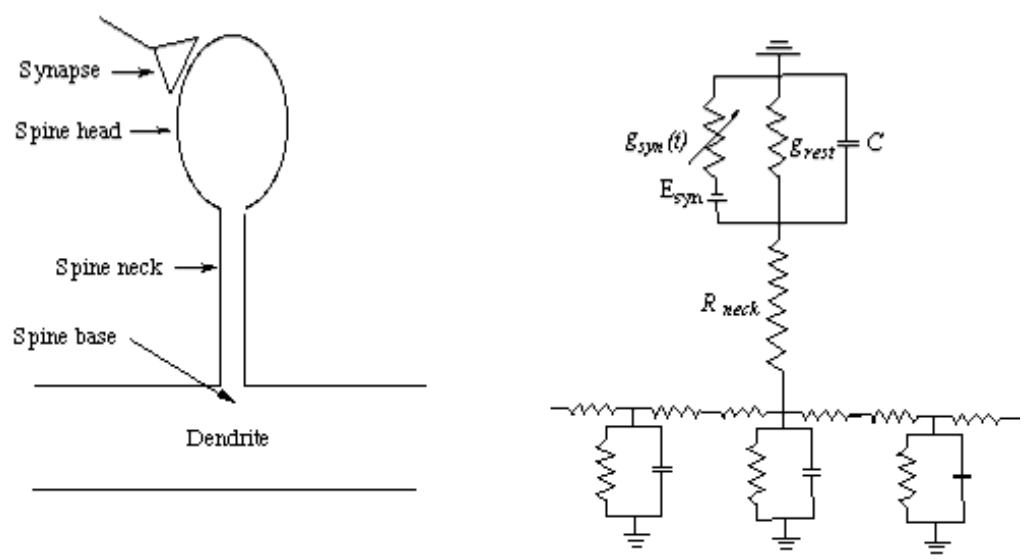
\includegraphics[scale=0.4]{03_15}
              \centering
          \end{figure}
          Here the factor \(F\) used in the
          other case can no longer be employed, as each spine exhibits its own kinetics.
\end{itemize}
\newpage

\section{Cable Theory Applied to Dendritic Structures}
\graphicspath{ {./images/04/} }
\subsection{The Cable Theory}
\subsubsection{Introduction}
The Cable Theory, first developed in 1850s and applied to neuroscience in 1930s and 1940s,
is based on a strong assumption: neuronal processes contain only voltage-independent
components. In other words, neurons are assumed to work exclusively as passive components,
therefore only resistances and capacitances are considered.\\
The following quantities represents the electrical components involved in the Cable Theory.
\begin{figure}[H]
    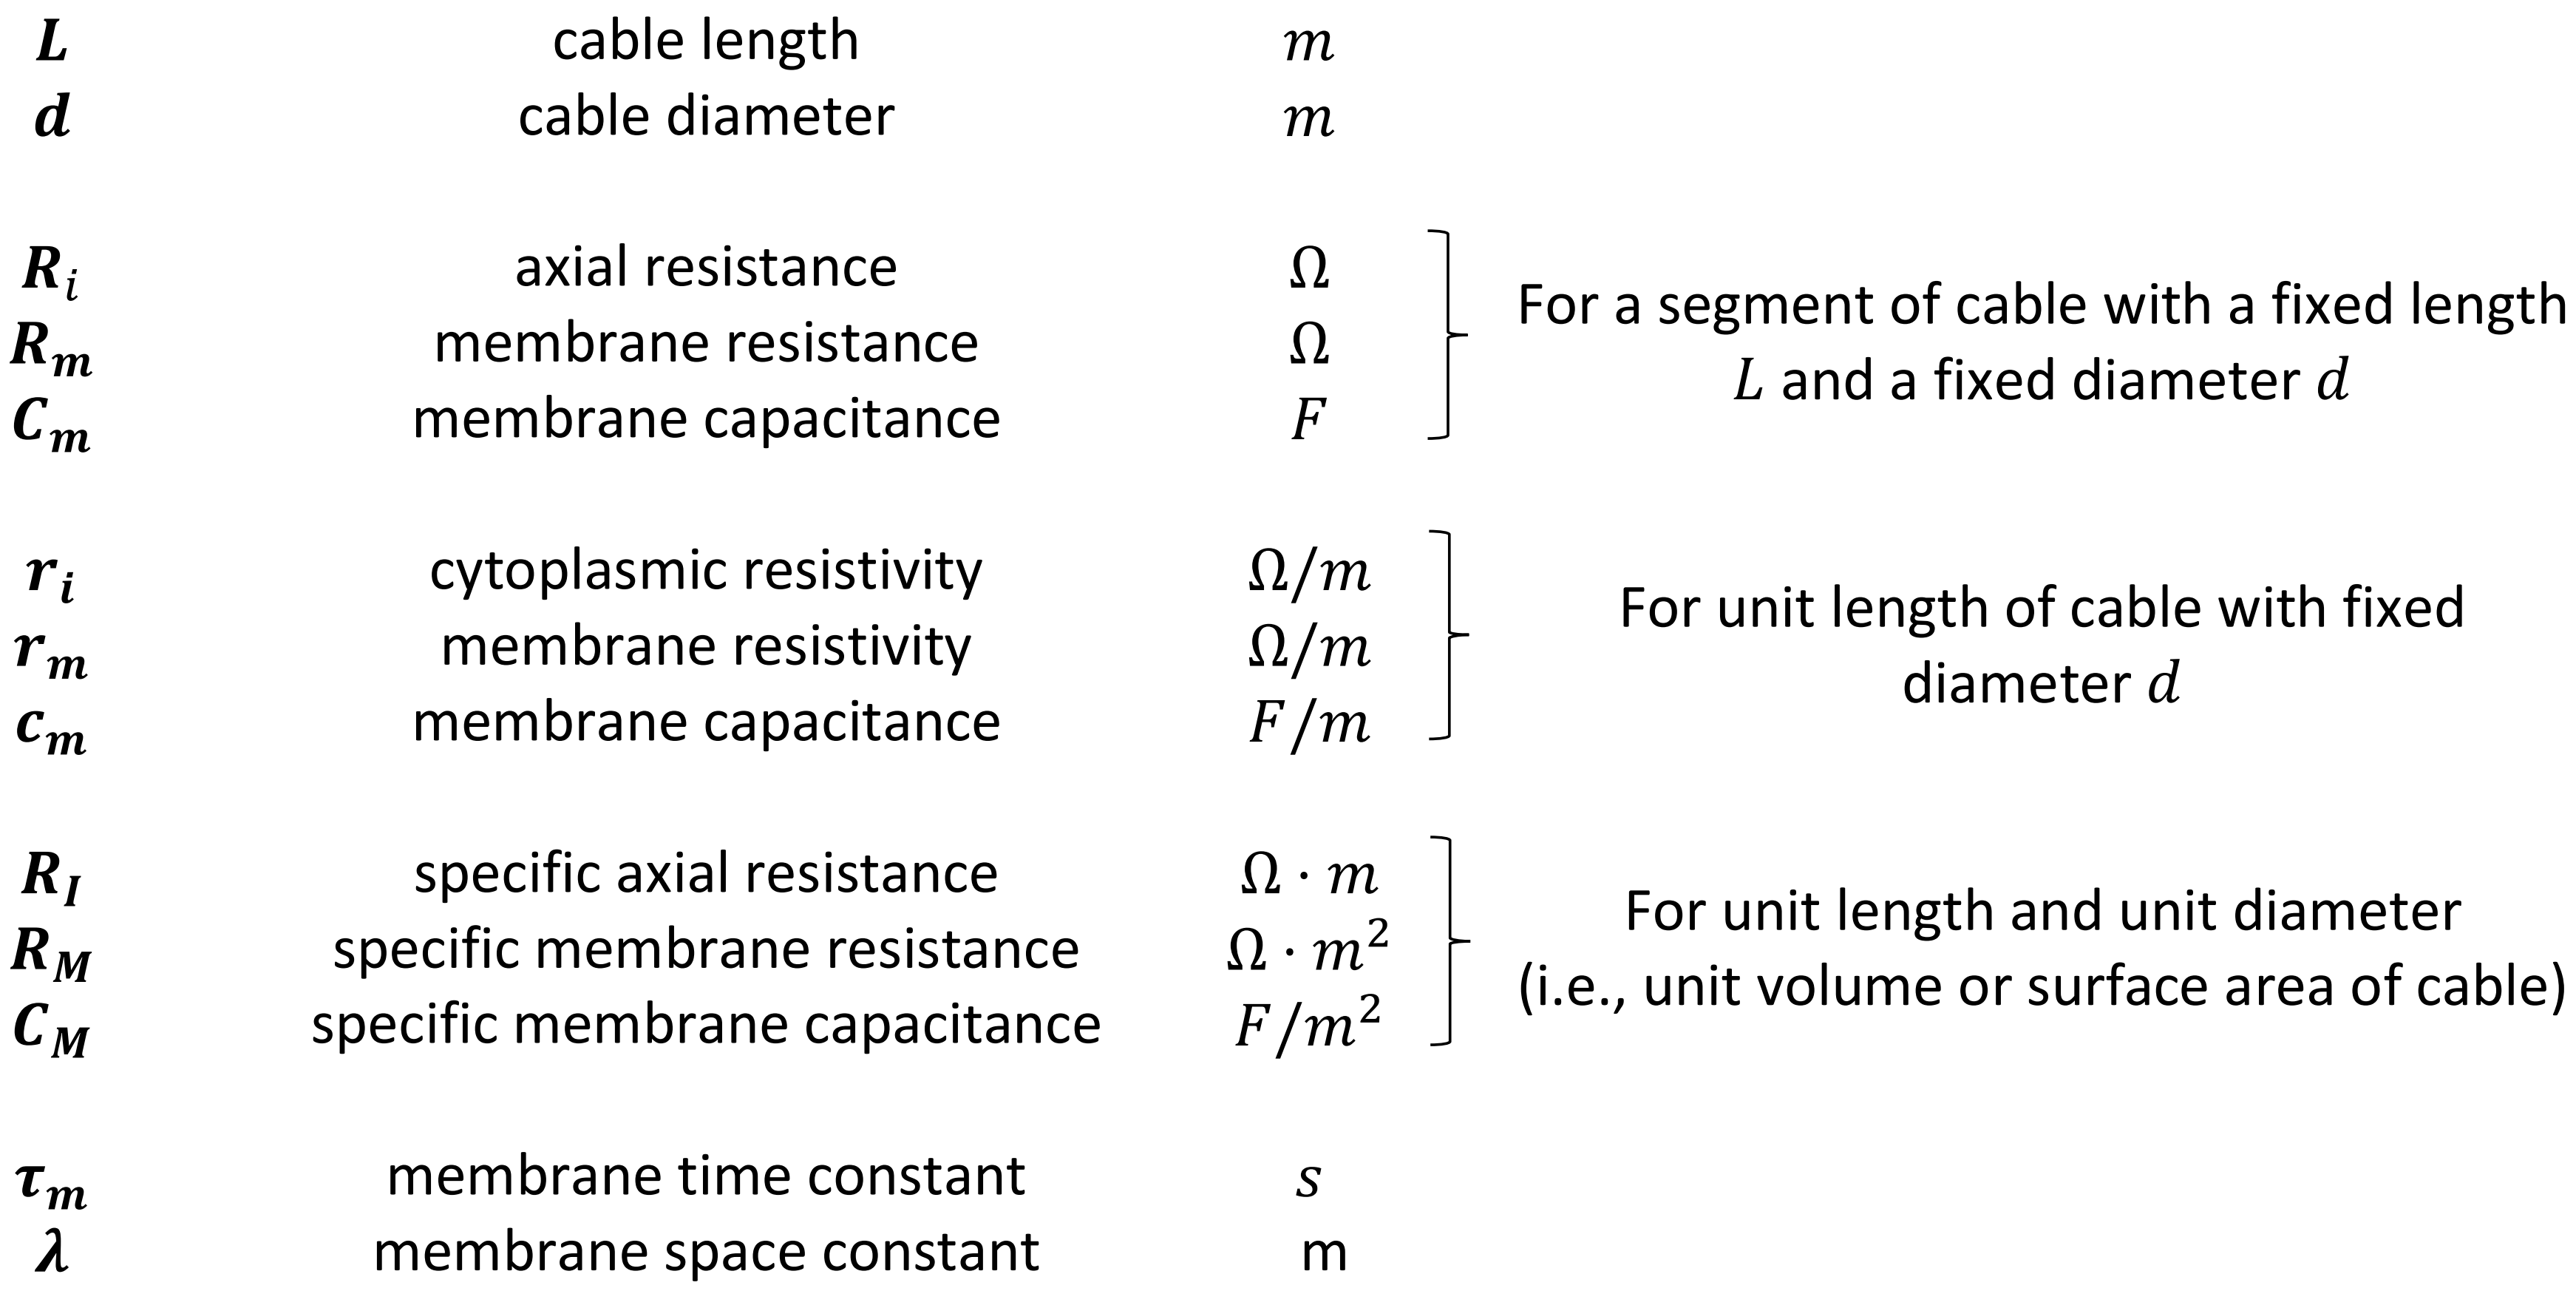
\includegraphics[scale=0.18]{04_1}
    \centering
\end{figure}
Note that given these measures, the relatonships reported here hold:
\begin{gather*}
    R_{i}=r_{i}L=\frac{4L}{\pi{d^2}}R_{I}
    \hspace{2cm}
    R_{m}=\frac{r_{m}}{L}=\frac{R_{M}}{\pi{dL}}
    \hspace{2cm}
    C_{m}=c_{m}L=\pi{dLC_{M}}\\
    \lambda=\sqrt{\frac{r_{m}}{r_{i}}}=\sqrt{\frac{d}{4}\frac{R_{M}}{R_{I}}}
    \hspace{2.5cm}
    \tau_{m}=r_{m}c_{m}=R_{M}C_{M}=R_{m}C_{m}
\end{gather*}
The cable is modelled as depicted below and the subsequent canonical expression for
the cable equation is derived.
\begin{figure}[H]
    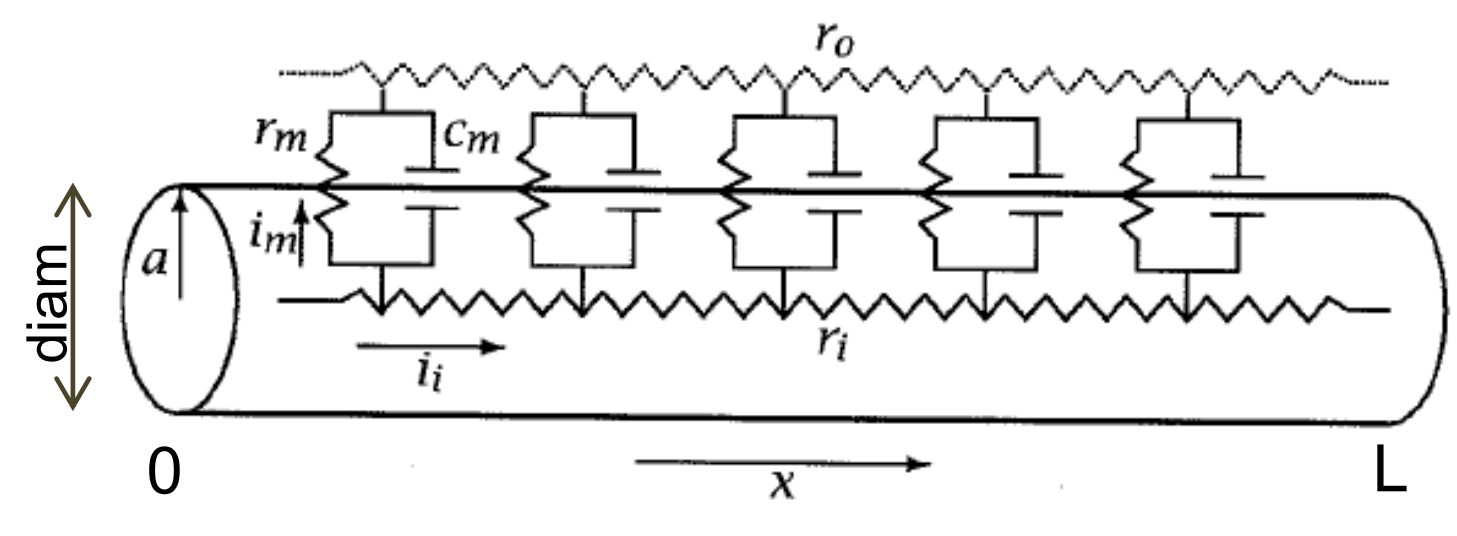
\includegraphics[scale=0.26]{04_2}
    \centering
\end{figure}
\begin{equation*}
    \lambda^{2}\frac{\partial^{2}V}{\partial{x^{2}}}-V-\tau{\frac{\partial{V}}{\partial{t}}}=0
    \Rightarrow
    \frac{\partial^{2}V}{\partial{X^{2}}}-V-\frac{\partial{V}}{\partial{T}}=0
\end{equation*}
Note that \(X=\frac{x}{\lambda}\) and \(T=\frac{t}{\tau}\), while \(V=(V_{i}-V_{e})-E_{r}\), with
\(V_i\) being the intracellular potential and \(V_e\) the extracellular one.
\subsubsection{Proof (Cable Equation Derivation)}
First of all, it is important to establish some hypotheses:
\begin{itemize}
    \item Neuronal processes contain only voltage-independent components, thus only passive
          electrical quantities are considered.
    \item The neurite is short (either axon or dendrites): \(L<\lambda\).
    \item The neurite length is much greater than its diameter: \(L>>d\).
    \item The propagation of the current is longitudinal, thus the current flows in parallel
          to the cylinder axis: \(r_{m}>>r_{i}\).
    \item The electrical properties of the membranes (\(r_{m}\), \(r_{i}\), \(c_{m}\)) are
          assumed to be uniform: \(V=V(t,x)\).
\end{itemize}
\begin{figure}[H]
    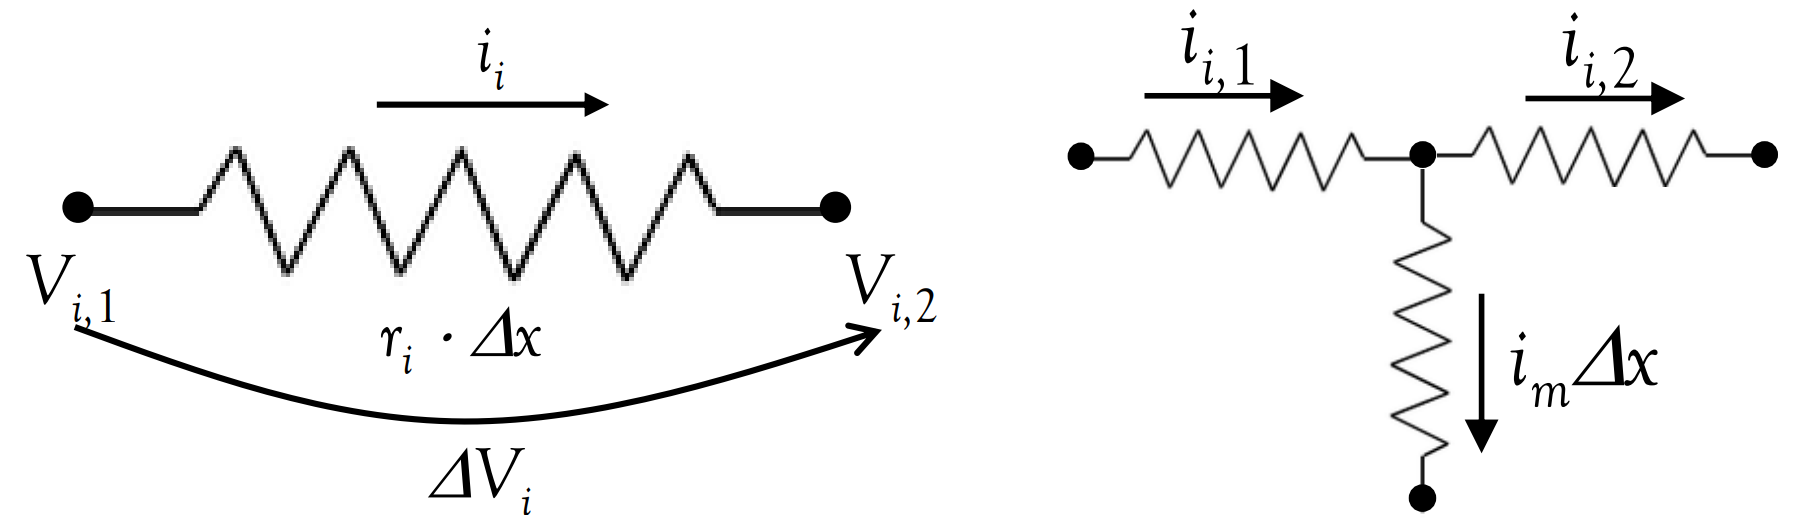
\includegraphics[scale=0.3]{04_3}
    \centering
\end{figure}
Due to the Ohm's Law:
\begin{equation*}
    i_{i}(r_{i}\Delta{x})=-\Delta{V_{i}}\Rightarrow\frac{\Delta{V_{i}}}{\Delta{x}}=-r_{i}i_{i}
\end{equation*}
Note that if \(\Delta{x}\) is infinitesimal (\(\Delta{x}\to{0}\)), this expression changes as:
\begin{equation*}
    \frac{\Delta{V_{i}}}{\Delta{x}}=-r_{i}i_{i}\Rightarrow\frac{\partial{V_{i}}}{\partial{x}}=-r_{i}i_{i}
\end{equation*}
Let's now derive the whole expression once again, without forgetting that \(r_{i}\) is uniform
by hypothesis:
\begin{equation*}
    \frac{\partial{V_{i}}}{\partial{x}}=-r_{i}i_{i}
    \Rightarrow
    \frac{\partial^{2}V_{i}}{\partial{x^{2}}}=-\frac{\partial{r_{i}i_{i}}}{\partial{x}}
    \Rightarrow
    \frac{\partial^{2}V_{i}}{\partial{x^{2}}}=-r_{i}\frac{\partial{i_{i}}}{\partial{x}}
\end{equation*}
At this point, some considerations can be done:
\begin{itemize}
    \item \(\frac{\partial{i_{i}}}{\partial{x}}=0\): there are no current variations
          within the increment \(\Delta{x}\).
    \item \(\frac{\partial{i_{i}}}{\partial{x}}<0\Rightarrow\frac{\partial^{2}V_{i}}{\partial{x^{2}}}>0\):
          there is an excess of current in the increment \(\Delta{x}\), thus an outward current \(i_{m}\) should
          be accounted for.
    \item \(\frac{\partial{i_{i}}}{\partial{x}}>0\Rightarrow\frac{\partial^{2}V_{i}}{\partial{x^{2}}}<0\):
          there is an entering current in the increment \(\Delta{x}\), indicating the presence of a synapse.
\end{itemize}
By applying the KCL, one can write that
\begin{equation*}
    i_{i,2}-i_{i,1}=-i_{m}\Delta{x}
    \Rightarrow
    \Delta{i_{i}}=-i_{m}\Delta{x}
    \Rightarrow
    -\frac{\Delta{i_{i}}}{\Delta{x}}=i_{m}
\end{equation*}
and if \(\Delta{x}\to{0}\) it becomes the following:
\begin{equation*}
    -\frac{\Delta{i_{i}}}{\Delta{x}}=i_{m}
    \Rightarrow
    -\frac{\partial{i_{i}}}{\partial{x}}=i_{m}
\end{equation*}
At this point, the resulting expression can be substituted into the previous one, leading to:
\begin{equation*}
    \frac{\partial^{2}V_{i}}{\partial{x^{2}}}=-r_{i}\frac{\partial{i_{i}}}{\partial{x}}
    \Rightarrow
    \frac{\partial^{2}V_{i}}{\partial{x^{2}}}=r_{i}i_{m}
    \Rightarrow
    \frac{1}{r_{i}}\frac{\partial^{2}V_{i}}{\partial{x^{2}}}=i_{m}
\end{equation*}
By reconsidering once again the previous hypotheses, it has been said that \(V=(V_{i}-V_{e})-E_{r}=V(x,t)\),
however the extracellular liquid is assumed to be isopotential, thus \(V_{e}\) and \(E_{r}\) are
independent on space \(x\) and time \(t\). As a consequence:
\begin{equation*}
    V=(V_{i}-V_{e})-E_{r}
    \Rightarrow
    V_{i}=V+V_{e}+E_{r}
    \Rightarrow
    \frac{\partial{V_{i}}}{\partial{x}}=\frac{\partial{V}}{\partial{x}}
\end{equation*}
Let's now take the previous equation and multiply it by \(r_{m}\):
\begin{equation*}
    \frac{1}{r_{i}}\frac{\partial^{2}V_{i}}{\partial{x^{2}}}\cdot{r_{m}}=i_{m}\cdot{r_{m}}
    \Rightarrow
    \frac{r_{m}}{r_{i}}\frac{\partial^{2}V}{\partial{x^{2}}}=r_{m}i_{m}
\end{equation*}
From now on, the \(i\)-th compartment depicted below is considered.
\begin{figure}[H]
    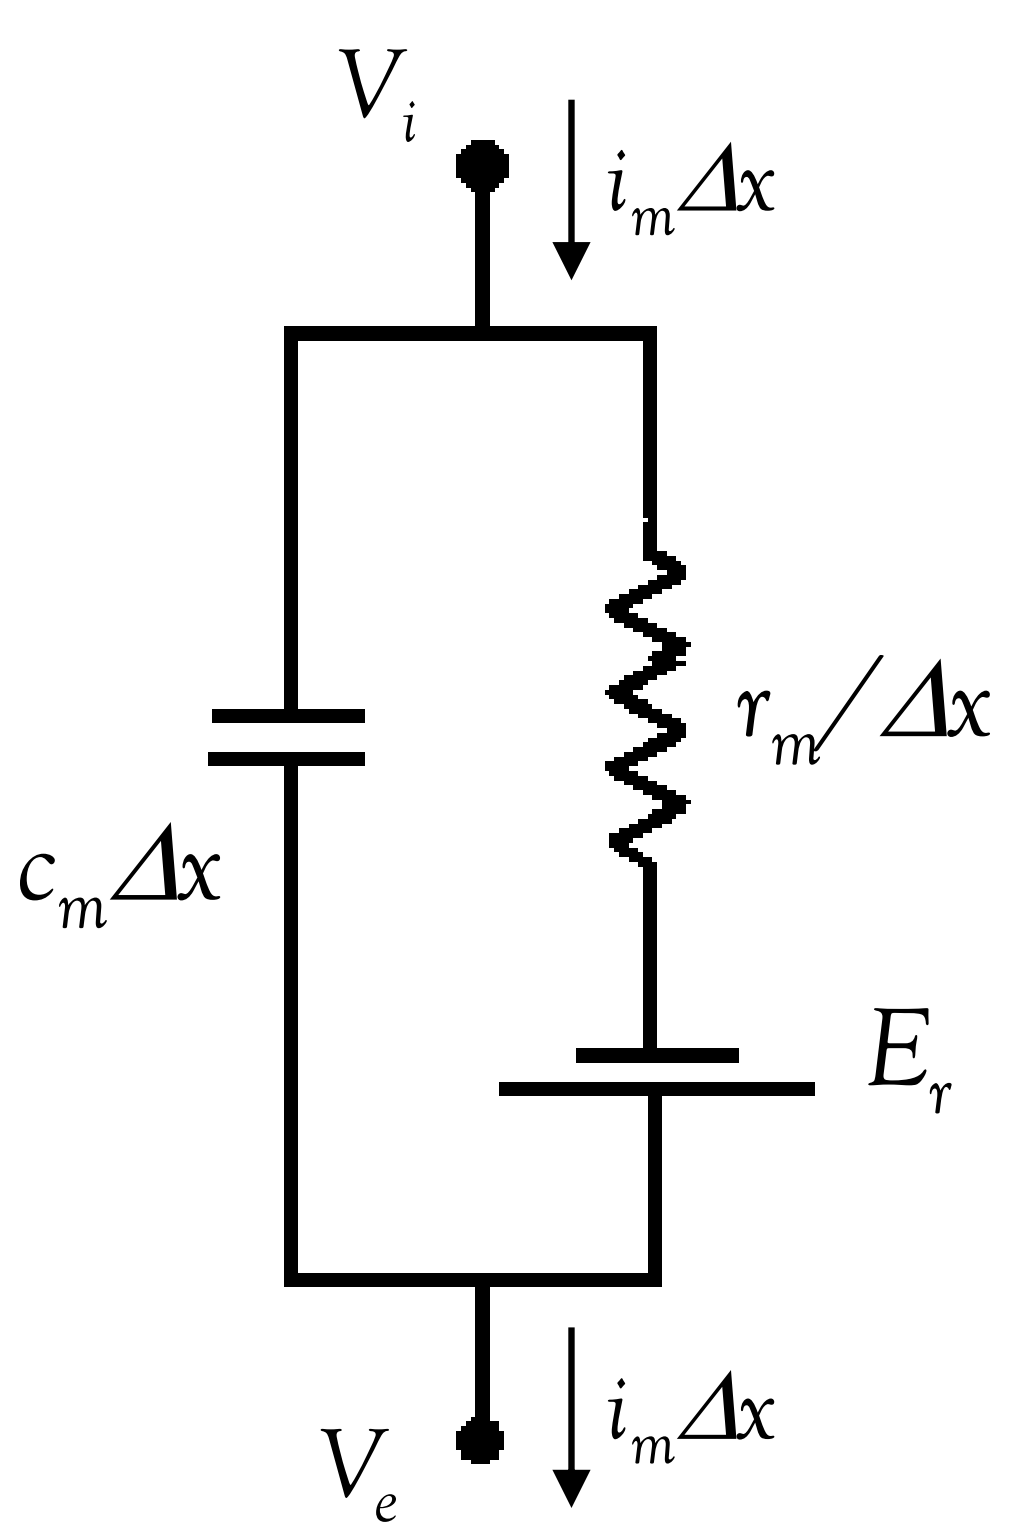
\includegraphics[scale=0.22]{04_4}
    \centering
\end{figure}
By considering its state equation, it can be said that:
\begin{equation*}
    i_{m}=c_{m}\frac{\partial{V}}{\partial{t}}+\frac{(V_{i}-V_{e})-E_{r}}{r_{m}}
    \Rightarrow
    r_{m}i_{m}=r_{m}c_{m}\frac{\partial{V}}{\partial{t}}+V
    \Rightarrow
    r_{m}i_{m}=\tau_{m}\frac{\partial{V}}{\partial{t}}+V
\end{equation*}
as the time constant is defined as \(\tau_{m}=r_{m}c_{m}\).\\
Since
\begin{equation*}
    \frac{r_{m}}{r_{i}}\frac{\partial^{2}V}{\partial{x^{2}}}=r_{m}i_{m}
    \hspace{1.5cm}
    \text{and}
    \hspace{1.5cm}
    \tau_{m}\frac{\partial{V}}{\partial{t}}+V=r_{m}i_{m}
\end{equation*}
it can be easily derived that
\begin{equation*}
    \frac{r_{m}}{r_{i}}\frac{\partial^{2}V}{\partial{x^{2}}}
    =
    \tau_{m}\frac{\partial{V}}{\partial{t}}+V
    \Rightarrow
    \lambda^{2}\frac{\partial^{2}V}{\partial{x^{2}}}-V-\tau_{m}\frac{\partial{V}}{\partial{t}}
    =
    0
\end{equation*}
with \(\lambda=\sqrt{\frac{r_{m}}{r_{i}}}\) being the space constant.
\subsubsection{Space and Time Constants}
\begin{itemize}
    \item \textbf{Space constant \(\lambda\)}: it depends not only on the axoplasmatic
          and membrane resistances (\(r_{i}\) and \(r_{m}\) respectively), but on the cable
          diameter as well, as illustrated by this relationship:
          \begin{equation*}
              \lambda=\sqrt{\frac{r_{m}}{r_{i}}}=\sqrt{\frac{R_{m}}{R_{i}}\frac{d}{4}}
          \end{equation*}
          In particular, cylinders with a bigger diameter tends to exhibit a bigger
          spatial constant, implying that the signal needs a greater distance to be attenuated.
    \item \textbf{Time constant \(\tau\)}: it defines the transient voltage response
          of a segment of the membrane to a current step input. It is formalized as:
          \begin{equation*}
              \tau=\tau_{m}=r_{m}c_{m}=R_{m}C_{m}=R_{M}C_{M}
          \end{equation*}
          Note that a bigger - i.e., slower - time constant implies a slower response to a
          changing stimulus.
\end{itemize}
Note that the \(\frac{\tau}{\lambda}\) ratio represents the time required for the voltage
across the membrane to reach \(\frac{1}{e}=0.37\) of its final value.\\
The obtained equivalent expressions
\begin{equation*}
    \lambda^{2}\frac{\partial^{2}{V}}{\partial{x^{2}}}-V-\tau\frac{\partial{V}}{\partial{t}}=0
    \hspace{2cm}
    \text{and}
    \hspace{2cm}
    \frac{\partial^{2}{V}}{\partial{X^{2}}}-V-\frac{\partial{V}}{\partial{T}}=0
\end{equation*}
are Partial Differential Equations (PDEs) and they were derived under the crucial
assumption that the axoplasmatic resistance \(r_{i}\) is uniform and constant: without this
hypothesis it is much more difficult to find a solution for the differential equation, as the
following term would change.
\begin{equation*}
    \frac{\partial^{2}V_{i}}{\partial{x^{2}}}=-r_{i}\frac{\partial{i_{i}}}{\partial{x}}
    \Rightarrow
    \frac{\partial^{2}V_{i}}{\partial{x^{2}}}=
    -r_{i}\frac{\partial{i_{i}}}{\partial{x}}-i_{i}\frac{\partial{r_{i}}}{\partial{x}}
\end{equation*}
As differential equations and time are involved, two kinds of solutions should be taken into
account:
\begin{itemize}
    \item \textbf{Steady-state solutions}
    \item \textbf{Time-dependent solutions}
\end{itemize}
\subsubsection{Cable Equation Steady-State Solutions}
In steady-state conditions, there is no change of voltage over time, therefore
the cable equation becomes an Ordinary Differential Equation (ODE):
\begin{equation*}
    \frac{\partial^{2}{V}}{\partial{X^{2}}}-V-\cancel{\frac{\partial{V}}{\partial{T}}}=0
    \Rightarrow
    \frac{\partial^{2}{V}}{\partial{X^{2}}}-V=0
\end{equation*}
The solution of such ODE can be equivalently expressed as:
\begin{itemize}
    \item \(V(X)=A_{1}e^{X}+A_{2}e^{-X}\)
    \item \(V(X)=B_{1}\cosh{(X)}+B_{2}\sinh{(X)}\)
    \item \(V(X)=C_{1}\cosh{(L-X)}+C_{2}\sinh{(L-X)}\)
\end{itemize}
where \(X=\frac{x}{\lambda}\) is the electrotonic coordinate and \(L=\frac{l}{\lambda}\)
is the electrotonic distance. Note that the solution will exhibit a sort of
expotential decay as the distance \(x\) from the input point increases.
\begin{figure}[H]
    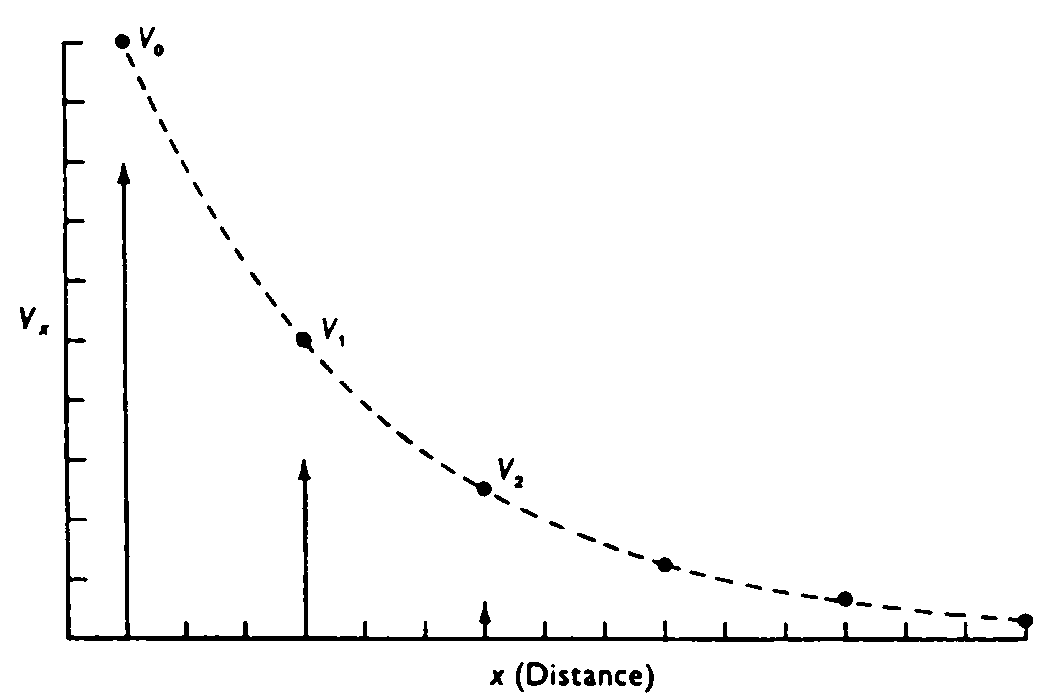
\includegraphics[scale=0.4]{04_5}
    \centering
\end{figure}
Several cases are considered in the following.
\paragraph{Semi-Infinite Cable} This model is not closed on the end side. The voltage
decays exponentially to zero as the distance from the current injection site is increased,
with a rate controlled by the space constant \(\lambda\).\\
\textit{Boundary Conditions:}
\begin{itemize}
    \item \(V(0)=V_{0}=\text{initial voltage}\)
    \item \(V(\infty)=0\)
\end{itemize}
\textit{General Solution:} \(V(X)=A_{1}e^{X}+A_{2}e^{-X}\)\\
\textit{Computations:}
\begin{gather*}
    V(X)\xrightarrow{X\to{\infty}}{0}
    \Rightarrow{0=A_{1}e^{X}+\cancelto{0}{A_{2}e^{-X}}}
    \Rightarrow{A_{1}e^{\infty}=0}
    \Rightarrow{A_{1}=0}\\
    V(X)\mid{}_{X=0}=V_{0}
    \Rightarrow{V_{0}=\cancel{A_{1}}+A_{2}}
    \Rightarrow{A_{2}=V_{0}}
\end{gather*}
\textit{Steady-State Solution:}
\begin{equation*}
    V(X)=V_{0}e^{-X}=V_{0}e^{-\frac{x}{\lambda}}
\end{equation*}
\paragraph{Finite Cable with Sealed End} The end of the cable is closed by an infinte
resistance \(R_{m}\), thus no axial current \(i_{i}\) flows at the end.\\
\textit{Boundary Conditions:}
\begin{itemize}
    \item \(V(0)=V_{0}=\text{initial voltage}\)
    \item \(i_{i}(L)=0\Rightarrow{\frac{\partial{V}}{\partial{X}}\mid{}_{X=L}=0}\)
\end{itemize}
\textit{General Solution:} \(V(X)=C_{1}\cosh{(L-X)}+C_{2}\sinh{(L-X)}\)\\
\textit{Computations:}
\begin{gather*}
    \frac{\partial{V}}{\partial{X}}\mid{}_{X=L}=0
    \Rightarrow{0=-\cancel{C_{1}\sinh{(L-L)}}-C_{2}\cosh{(L-L)}}
    \Rightarrow{0=C_{2}\cancelto{1}{\cosh{(0)}}}
    \Rightarrow{C_{2}=0}\\
    V(0)=V_{0}
    \Rightarrow{C_{1}\cosh{(L)}+\cancel{C_{2}\sinh{(L)}}}
    \Rightarrow{C_{1}=\frac{V_{0}}{\cosh{(L)}}}
\end{gather*}
\textit{Steady-State Solution:}
\begin{equation*}
    V(X)=V_{0}\frac{\cosh{(L-X)}}{\cosh{(L)}}
\end{equation*}
\paragraph{Finite Cable with Open End} This model is cut open at the end, providing
a short circuit to the ground - i.e., the extracellular potential.\\
\textit{Boundary Conditions:}
\begin{itemize}
    \item \(V(0)=V_{0}=\text{initial voltage}\)
    \item \(V(L)=0\)
\end{itemize}
\textit{General Solution:} \(V(X)=C_{1}\cosh{(L-X)}+C_{2}\sinh{(L-X)}\)\\
\textit{Computations:}
\begin{gather*}
    V(L)=0
    \Rightarrow{0=C_{1}\cancelto{1}{\cosh{(0)}}+\cancel{C_{2}\sinh{(0)}}}
    \Rightarrow{C_{1}=0}\\
    V(0)=V_{0}
    \Rightarrow{V_{0}=\cancel{C_{1}\cosh{(L)}}+C_{2}\sinh{(L)}}
    \Rightarrow{C_{2}=\frac{V_{0}}{\sinh{(L)}}}
\end{gather*}
\textit{Steady-State Solution:}
\begin{equation*}
    V(X)=V_{0}\frac{\sinh{(L-X)}}{\sinh{(L)}}
\end{equation*}
\paragraph{Finite Cable with Clamped End} The end of the cable is clamped
at an arbitrary voltage \(V_{L}\), it can be seen as a generalization of
the open end case, where \(V_{L}=0\).\\
\textit{Boundary Conditions:}
\begin{itemize}
    \item \(V(0)=V_{0}=\text{initial voltage}\)
    \item \(V(L)=V_{L}\)
\end{itemize}
\textit{General Solution:} \(V(X)=C_{1}\cosh{(L-X)}+C_{2}\sinh{(L-X)}\)\\
\textit{Computations:}
\begin{gather*}
    V(L)=V_{L}
    \Rightarrow{V_{L}=C_{1}\cancelto{1}{\cosh{(0)}}+\cancel{C_{2}\sinh{(0)}}}
    \Rightarrow{C_{1}=V_{L}}\\
    V(0)=V_{0}
    \Rightarrow{V_{0}=C_{1}\cosh{(L)}+C_{2}\sinh{(L)}}
    \Rightarrow{C_{2}=\frac{V_{L}}{\tanh{(L)}}}
\end{gather*}
\textit{Steady-State Solution:}
\begin{equation*}
    V(X)=V_{L}\cosh{(L-X)}+\frac{V_{L}}{\tanh{(L)}}\sinh{(L-X)}
\end{equation*}
All the presented steady-state solutions are presented in the plot below, showing
how the voltage drops as a function of distance.
\begin{figure}[H]
    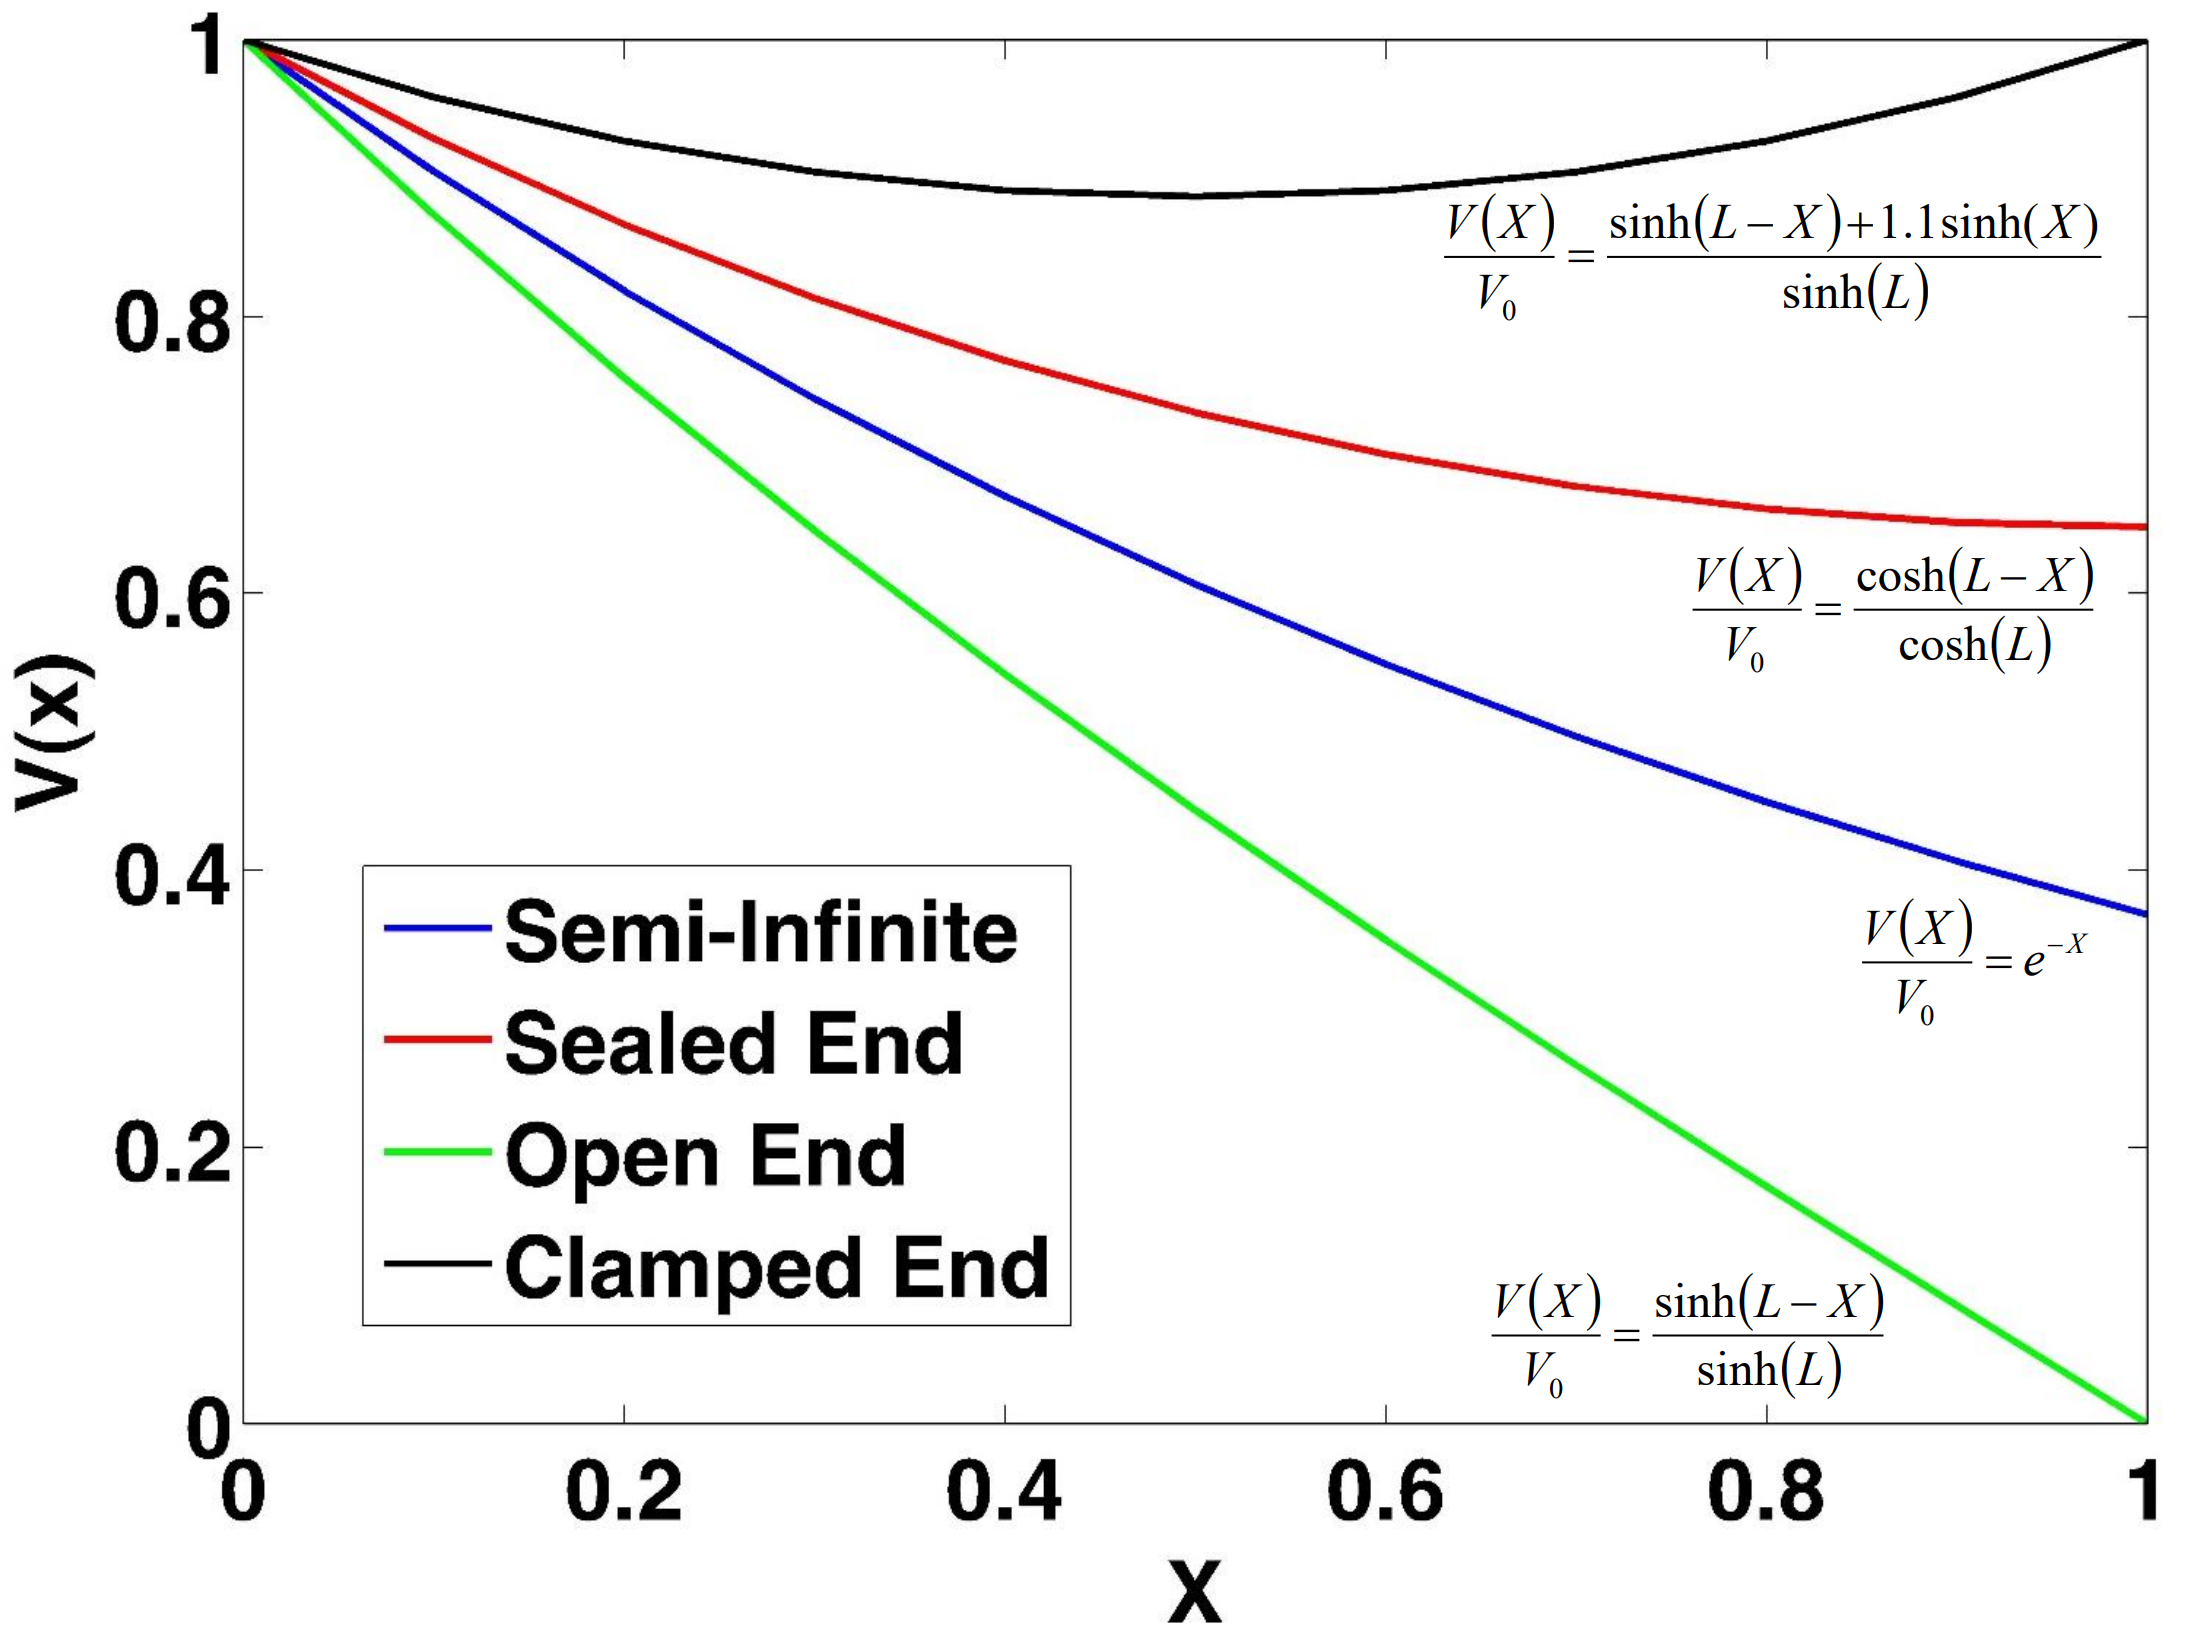
\includegraphics[scale=0.25]{04_6}
    \centering
\end{figure}
Finally, there are also two other cases of finite cable that should be taken into
account:
\begin{itemize}
    \item \textbf{Finite Cable with Leaky End}: the boundary conditions are defined
    by the same expression
    \begin{equation*}
        \pm{\frac{1}{r_{i}}\frac{\partial{V}}{\partial{x}}}\mid{}_{x=0,L}=G_{L}\cdot{V(x,t)}
    \end{equation*}
    with \(G_{L}\) being a conductance which connects the end of the cable to the resting
    potential \(E_{r}\).
    \item \textbf{Finite Cable with Current Injected at Sealed End}: the boundary conditions
    are defined by the same expression
    \begin{equation*}
        \pm{\frac{1}{r_{i}}\frac{\partial{V}}{\partial{x}}}\mid{}_{x=0,L}=I(t)
    \end{equation*}
\end{itemize}
Notice that this is used to model a dendrite stimulated from one extremity to the other
and vice-versa, in order to obtain information on the dendrite properties (collision test).
\subsubsection{Cable Equation Time-Dependent Solutions}
Firstly, let's make an hypothesis: the membrane potential is isopotential, thus it
is constant across the space, in other words \(\frac{\partial{V}}{\partial{X}}=0\).
Said so, the cable equation is simplified as follow:
\begin{equation*}
    \cancel{\frac{\partial^{2}{V}}{\partial{X^{2}}}}-V-\frac{\partial{V}}{\partial{T}}=0
    \Rightarrow
    \frac{\partial^{2}{V}}{\partial{T^{2}}}+V=0
\end{equation*}
If an isopotential neuron is stimulated by a current pulse \(I_{0}\), then:
\begin{equation*}
    V(T)=I_{0}R_{m}(1-e^{-T})
\end{equation*}
where \(R_{m}\) is the membrane resistance of the isopotential segment.\\
Whenever the stimulus is removed, the voltage decays exponentially from
its maximum value \(V(t_{0})=V_{0}\):
\begin{equation*}
    V(T)=V_{0}e^{-T}=V_{0}e^{-\frac{t}{\tau}}
\end{equation*}
In the general case of passive cylinders, thus considering both space and
time constants, the solution of the cable equation \(V(X,T)\) can be expressed as
a sum of an infinite number of exponential decays.

\subsection{The Computational Properties of Dendrites}
When talking about dendrites one may ask whether they are somehow
important from the functional point of view or, on the other hand,
if they play only a key role in forming connections, without any
contribution in computations. With respect to how the brain process
information there are two main viewpoints:
\begin{itemize}
    \item Information processing results primarily from the properties of
    synapses and the connectivity of neurons. The contribution of a single
    neuron is negligible, the emphasis is on the complexity of the overall
    network.
    \item The focus should be on the neuron, playing a fundamental role in the
    computations, thanks to its complex morphology.
\end{itemize}
This second viewpoint is a little old-fashioned nowadays, as it was at the base
of the perceptrons, which aimed at describing the biological neurons and their
computational capabilities in a comprehensive way. The idea was that neurons are
able to operate as devices where analog computations are at a certain point
transformed into a digital output signal.\\
However, today it is mostly believed that linear and non-linear mechanisms
in the dendritic tree are likely to serve as computational building blocks:
combined together they play a key role in the overall computation performed
by a neuron.
\subsubsection{Passive Dendrites}
\paragraph{Passive Filters} They may act as linear filters acting on the input signal: this
kind of filtering tends to attenuate the dendritic signal as a function of the travelled
distance and its frequency. As a consequence, if a signal is too low in power or very
far away it tends to be disregarded.
\paragraph{Non-linear Interactions} Whenever excitatory and inhibitory inputs are
widely separated from one another on different dendritic branches, the input signals
will tend to sum linearly at the soma (a logic OR).\\
If the inputs are adjacent to each other the inhibition can produce a highly non-linear
shunting of the excitatory input (a logic AND-NOT).\\
Moreover, the branch points in the dendritic tree sums up the currents in individual
branches.
\paragraph{Reducing and Amplifying the Mutual Interaction} Generally, excitatory
inputs to the same branch tend to sum sublinearly, whereas inputs on different branches
sum linearly.
\paragraph{Coincidence Detection} The back-propagation of action potentials triggers
a dendritic Ca\({}^{2+}\) spike which depolarizes the whole apical dendrite and drives
a burst of spikes in the axon.
\begin{figure}[H]
    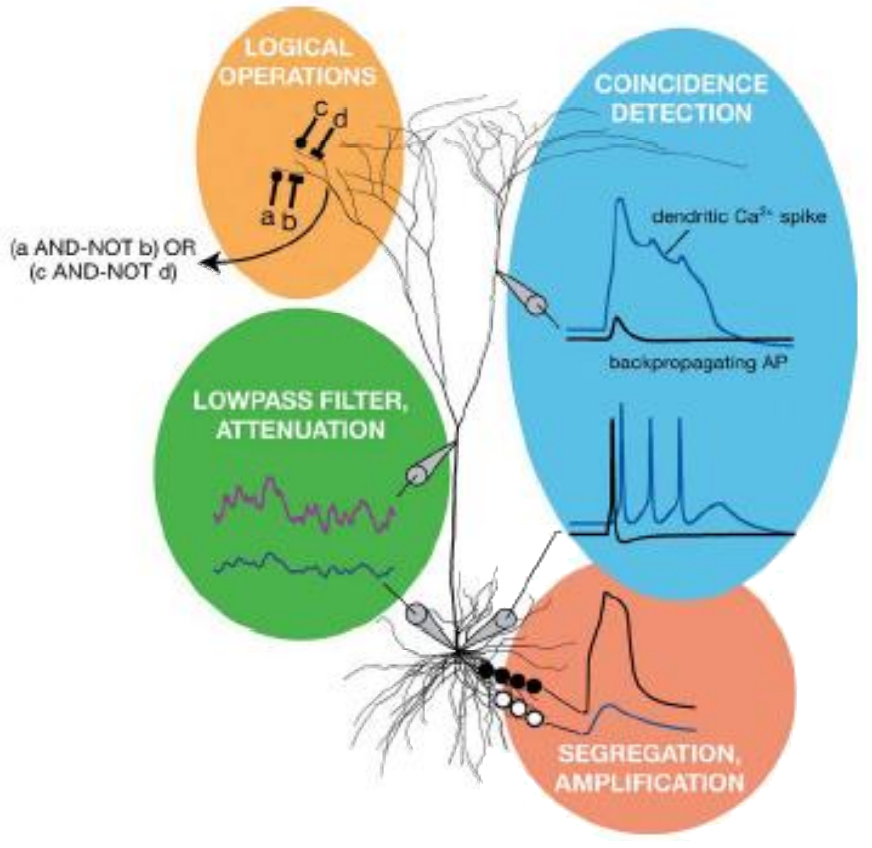
\includegraphics[scale=0.5]{04_7}
    \centering
\end{figure}
\subsubsection{Active Dendrites}
\paragraph{Dynamic Polarization Law} In the nervous system information flows in one
direction, from dendrites to the soma and then to the axon.
\paragraph{Back-propagation Theory} The presence of excitable ionic currents in the
dendrites supports dendritic action potentials that travel in the reverse direction
w.r.t. the main one. Therefore, the neuron is no longer considered to be an
open-loop system, but it presents an internal feedback mechanism.\\
In general, the amount of input is critical in defining the direction of
propagation, while the kind of computation performed is a consequence of
the dendritic tree morphology.
\newpage

\section{The Hodgkin-Huxley Model}
\graphicspath{ {./images/05/} }
Prior to 1940, there were no hints regarding the underlying mechanism of a neuron
as only extracellular recordings were available. At that time it was known that:
\begin{enumerate}
    \item The cell membrane separates solutions with different ionic concentrations.
    \item \([\text{K}^{+}]_{o}<<[\text{K}^{+}]_{i}\)
    \item \([\text{Na}^{+}]_{o}>>[\text{Na}^{+}]_{i}\)
\end{enumerate}
Moreover, the neuronal activity was believed to be a breakdown of the membrane resistance.\\
Then, the voltage clamp technique was introduced, enabling to maintain the membrane
voltage \(V_{m}\) at any desired level. Thus, it allowed, together with chemical stimulation,
to study the effect of each kind of ion via a selective analysis of the single ionic currents.
As a matter of fact, it was observed that both Na\({}^{+}\) and K\({}^{+}\) ions make significant
contributions to the ionic current underlying the action potential. Therefore, there are changes
in the membrane permeabilities for a few different ions, not for all ions, as thought before.\\
In particular, the action potential amplitude crtically depends on the external concentration of
Na\({}^{+}\) ions.\\
In the classical patch-clamp technique, scientists were able to analyse a patch of cellular membrane
and selectively block some kinds of channels, studying how the behaviour of the remaining ones would
affect the \(V_{m}\) voltage. However, Neher and Sakmann improved such a technique and allowed to
measure the effect on \(V_{m}\) of a single ion channel.\\
Hence, the big remaining question investigated by Hodgkin and Huxley was how the permeability of the
membrane to specific ions is linked to \(V_{m}\) and time. The two researchers managed to
disentangle the temporal contributions of different ions assuming that they responded
differently to changes in \(V_{m}\).
\begin{figure}[H]
    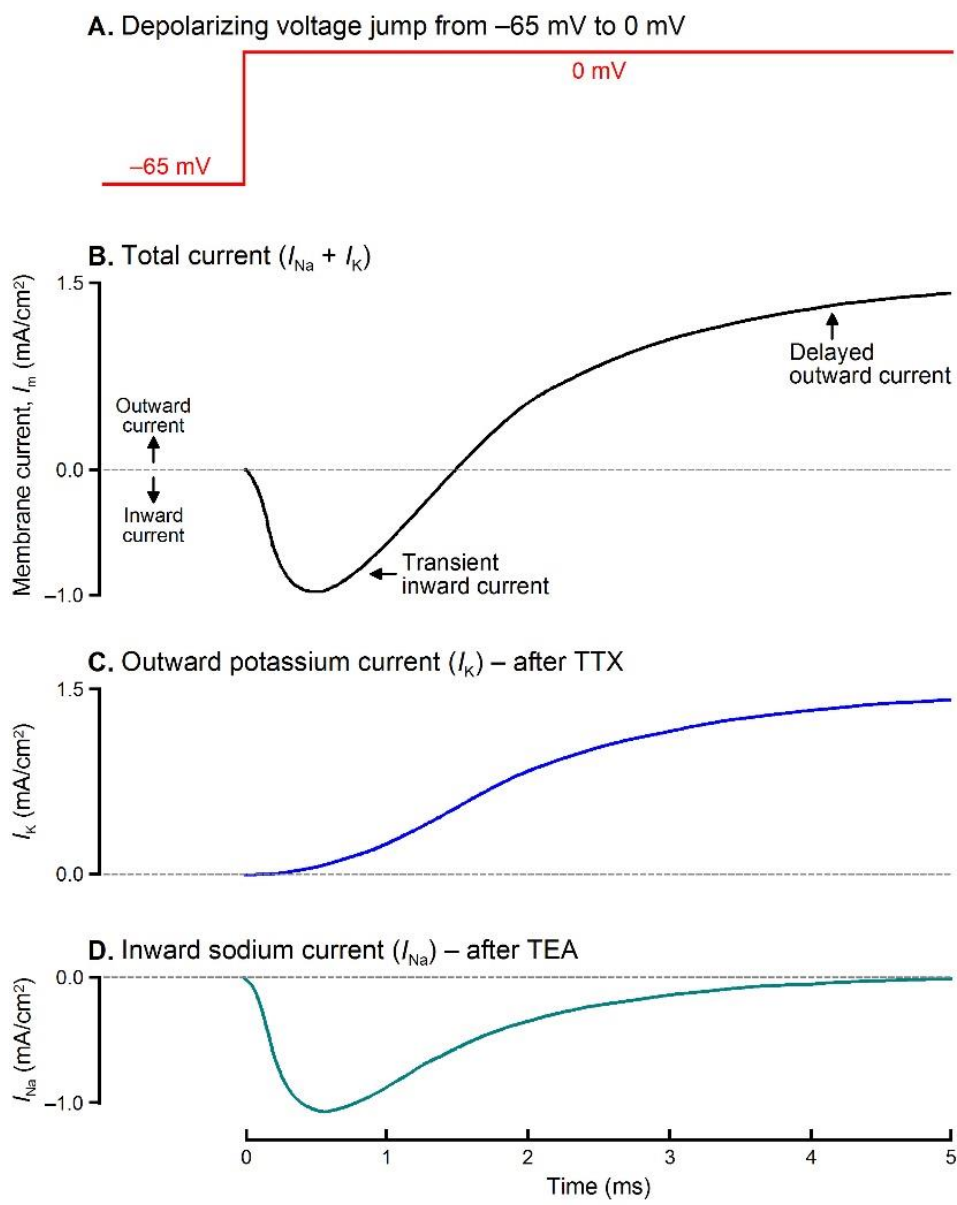
\includegraphics[scale=0.33]{05_1}
    \centering
\end{figure}

\subsection{Equivalent Circuit}
The following equivalent may be used to model virtually any cellular membrane, in particular it
can describe a neuron membrane if the proper ionic channels - i.e., Na\({}^{+}\) and K\({}^{+}\) -
are introduced. Note that also a leakage current \(I_{leak}\) is considered.
\begin{figure}[H]
    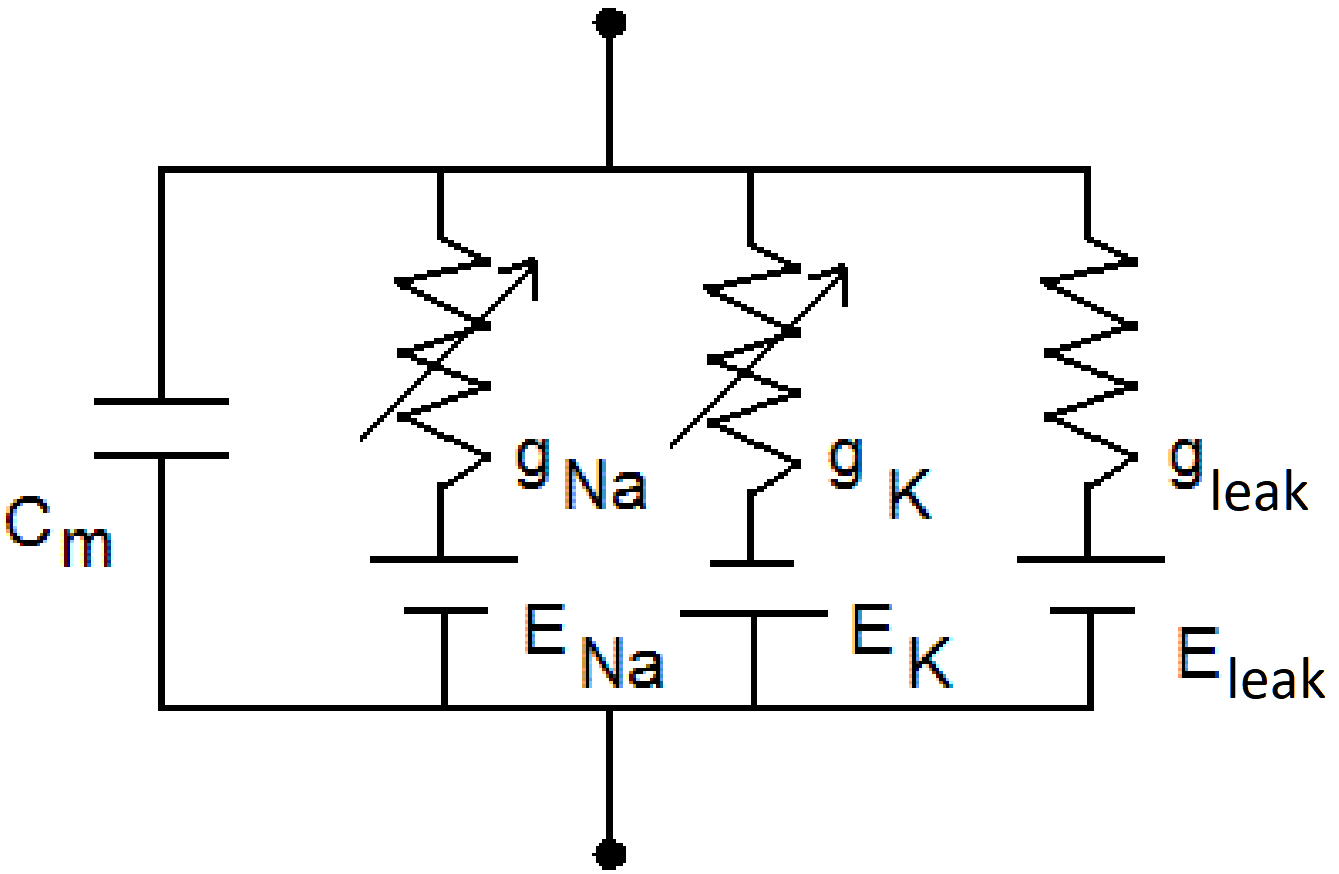
\includegraphics[scale=0.22]{05_2}
    \centering
\end{figure}
Thus, the membrane current is described as:
\begin{equation*}
    I_{m}(t)=I_{ionic}(t)+C_{m}\frac{dV_{m}}{dt}=I_{Na}+I_{K}+I_{leak}+C_{m}\frac{dV_{m}}{dt}
\end{equation*}
Let's now take one of the three ionic current components, for instance Na\({}^{+}\), hence
the sodium current \(I_{Na}\) can be computed thanks to the Ohm's Law:
\begin{equation*}
    I_{Na}(t)=g_{Na}(V_{m}(t),t)\cdot{\bigl[V_{m}(t)-E_{Na}\bigr]}
\end{equation*}
with \(E_{Na}\) being the sodium reversal potential obtained from the Nernst Equation:
\begin{equation*}
    E_{Na}=\frac{RT}{zF}\ln{\frac{[Na]_{o}}{[Na]_{i}}}
\end{equation*}
Therefore, it is clear that sodium and potassium conductances are functions of
both time and membrane voltage, as shown in the image below.
\begin{figure}[H]
    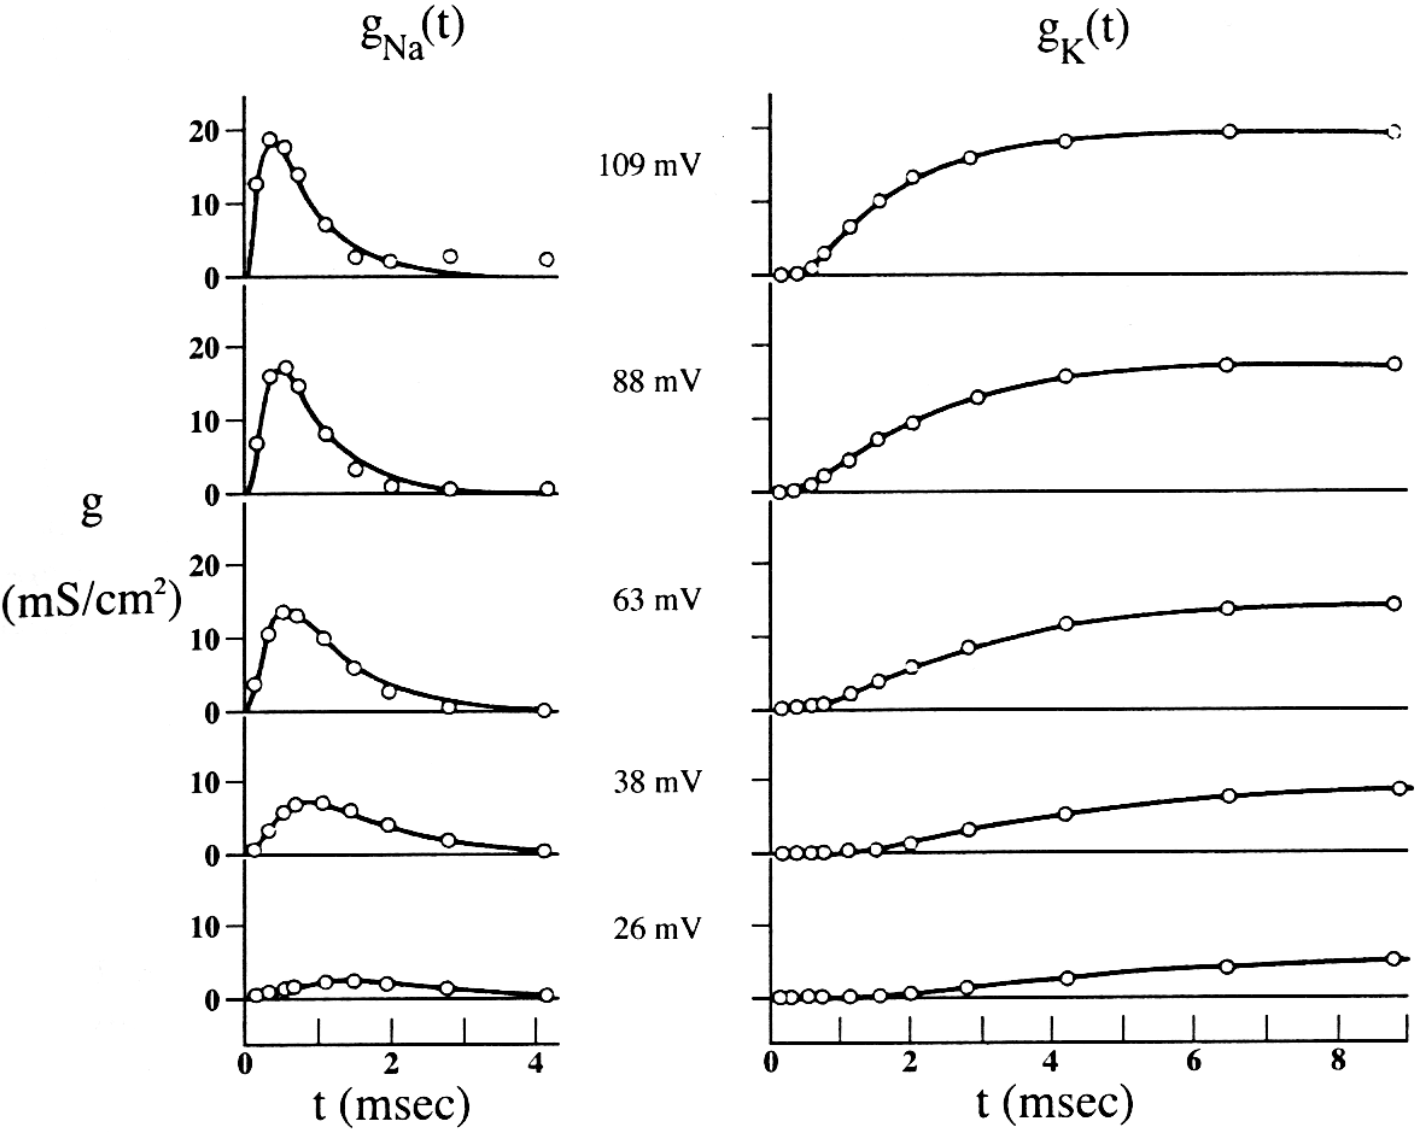
\includegraphics[scale=0.3]{05_3}
    \centering
\end{figure}
Note that the potassium channels dynamics is monophasic - i.e., monotonic - and is delayed
w.r.t. the sodium channels response, in addition it shows no decay.

\subsection{Gating Particles}
The gating particles (\(m\), \(h\), \(n\), \dots) were introduced to describe the dynamics of
the ionic conductances, they can be either activating or inactivating.
\begin{equation*}
    g_{Na}=\bar{g}_{Na}\cdot{m^{3}h}
    \hspace{3cm}
    g_{K}=\bar{g}_{K}\cdot{n^{4}}
\end{equation*}
The sodium kinetics is governed by 2 gating particles, thus its behaviour is biphasic. On the other
hand, the potassium dynamics is monophasic, as it depends only on \(n\).\\
Note that a gating particle \(p_{i}\) value is in the \([0; 1]\) interval and it can be equivalently
seen as the fraction or the probability of gates of type \(i\) being open. On the contrary,
\((1-p_{i})\) represents the fraction of type \(i\) gates being closed.\\
The connection between these two probabilities is governed by two functions:
\(\alpha_{i}(V_{m})\) and \(\beta_{i}(V_{m})\).
Now, this differential equation describing how \(p_{i}\) evolves over time can be derived:
\begin{equation*}
    \frac{dp_{i}}{dt}=\alpha_{i}(V_{m})(1-p_{i})-\beta_{i}(V_{m})p_{i}
\end{equation*}
The steady-state solution \(p_{i_{\infty}}\) is
\begin{equation*}
    p_{i_{\infty}}(V_{m})=\frac{\alpha_{i}(V_{m})}{\alpha_{i}(V_{m})+\beta_{i}(V_{m})}
\end{equation*}
while the time constant for the channels of type \(i\) is
\begin{equation*}
    \tau_{i}(V_{m})=\frac{1}{\alpha_{i}(V_{m})+\beta_{i}(V_{m})}
\end{equation*}
\paragraph{Potassium Current}
\begin{equation*}
    I_{K}=g_{K}(V_{m}-E_{K})=\bar{g}_{K}\cdot{n^{4}}\cdot{(V_{m}-E_{K})}
\end{equation*}
where \(\bar{g}_{K}=36\;mS/cm^{2}\).\\
\(n\) is an \textbf{activating} particle, where the two \(\alpha_{n}\) and \(\beta_{n}\)
functions are:
\begin{equation*}
    \alpha_{n}(V_{m})=\frac{10-V_{m}}{100\cdot\bigl(e^{\frac{10-V_{m}}{10}}-1\bigr)}
    \hspace{3cm}
    \beta_{n}(V_{m})=0.125\cdot{e^{-\frac{V_{m}}{80}}}
\end{equation*}
with \(\alpha_{n}\) being a sigmoidal function and \(\beta_{n}\) an exponential-like function.
Finally, the time-dependent solution can be written as:
\begin{equation*}
    n(t)=n_{\infty}-(n_{\infty}-n_{0})e^{-\frac{t}{\tau_{n}}}
\end{equation*}
\paragraph{Sodium Current}
\begin{equation*}
    I_{Na}=g_{Na}(V_{m}-E_{Na})=\bar{g}_{Na}\cdot{m^{3}h}\cdot{(V_{m}-E_{Na})}
\end{equation*}
where \(\bar{g}_{Na}=120\;mS/cm^{2}\).\\
\(m\) is an \textbf{activating} particle, where the two \(\alpha_{m}\) and \(\beta_{m}\)
functions are:
\begin{equation*}
    \alpha_{m}(V_{m})=\frac{25-V_{m}}{10\cdot\bigl(e^{\frac{25-V_{m}}{10}}-1\bigr)}
    \hspace{3cm}
    \beta_{m}(V_{m})=4\cdot{e^{-\frac{V_{m}}{18}}}
\end{equation*}
\(h\) is an \textbf{inactivating} particle, where the two \(\alpha_{h}\) and \(\beta_{h}\)
functions are:
\begin{equation*}
    \alpha_{h}(V_{m})=0.07\cdot{e^{-\frac{V_{m}}{20}}}
    \hspace{3cm}
    \beta_{h}(V_{m})=\frac{1}{e^{\frac{30-V_{m}}{10}}+1}
\end{equation*}
Finally, the following two plots are derived. The first one depicts the gating particles
time constants vs. the membrane voltage \(V_{m}\) and it can be seen that \(m\) has a
super fast dynamics when compared to the other two particles. The second plot shows
the gating particles activating or inactivating effect as a function of the membrane
voltage \(V_{m}\).
\begin{figure}[H]
    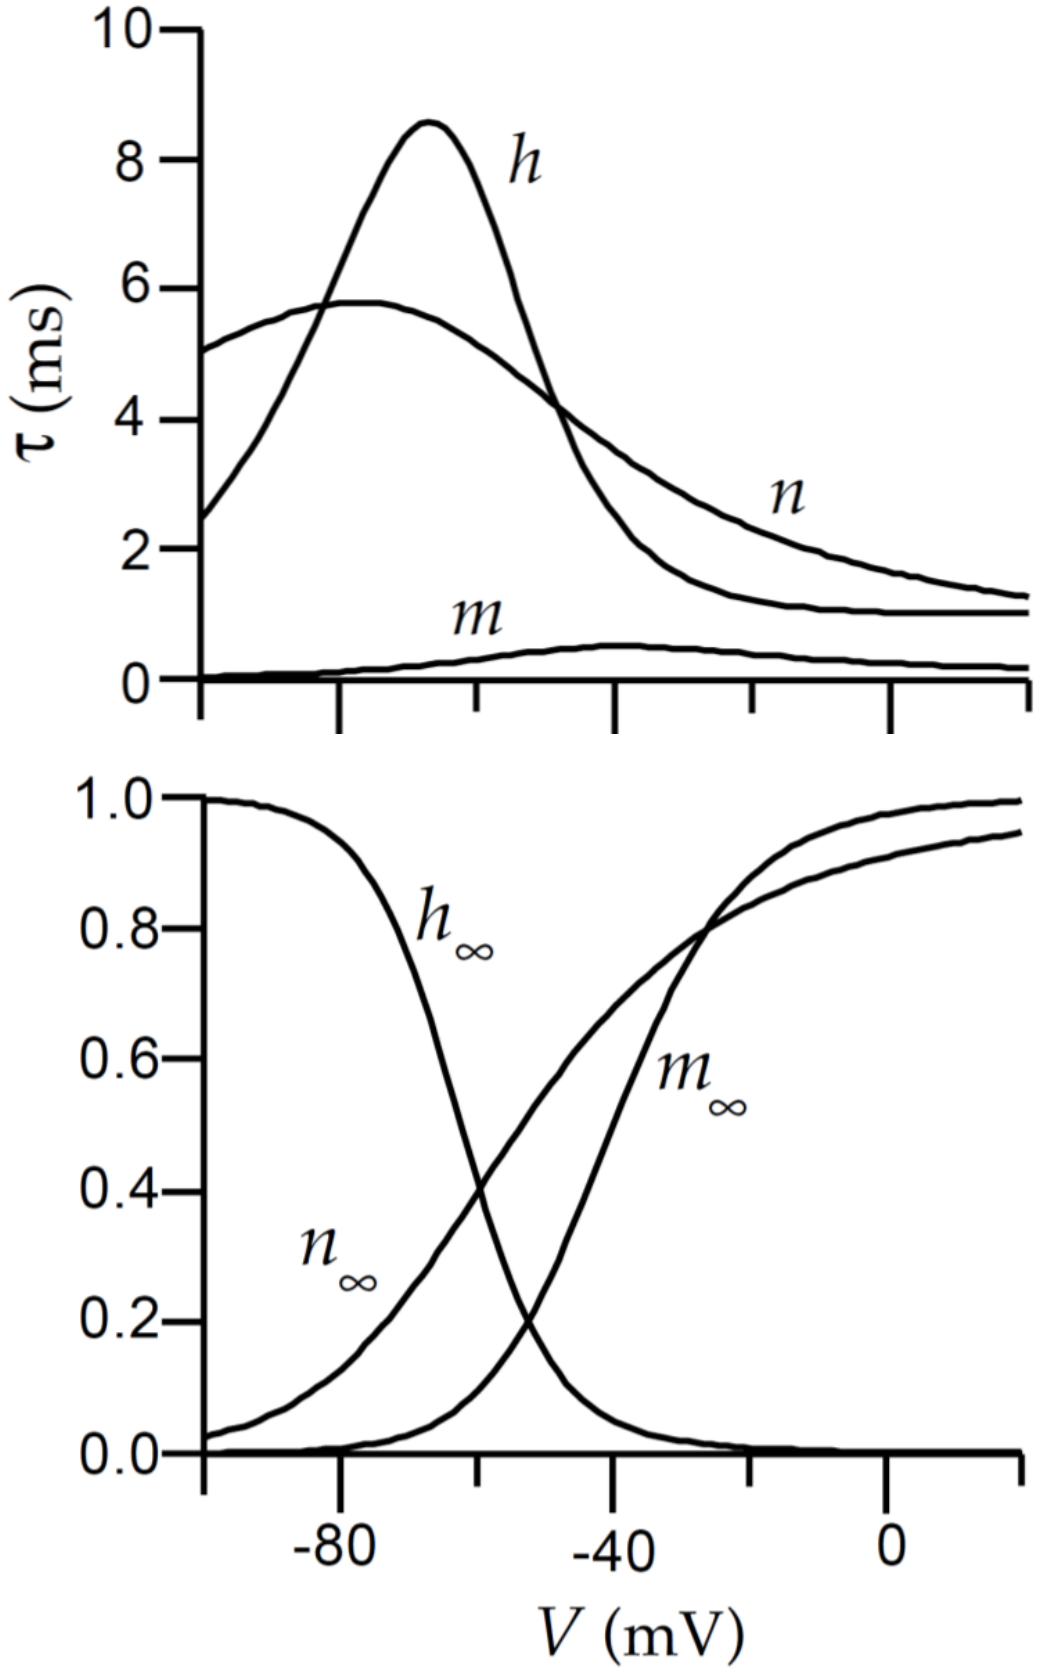
\includegraphics[scale=0.28]{05_4}
    \centering
\end{figure}
In the following it is instead shown what happens to the ionic currents (A), to the
membrane potential \(V_{m}\) (B), and to the gating particles respectively in two distinct
cases:
\begin{itemize}
    \item \textit{Solid} lines: the input current pulse overcomes the threhsold and generates
          an action potential (suprathreshold stimulus).
    \item \textit{Dashed} lines: the input current pulse is not high enough to produce an
          action potential (subthreshold stimulus).
\end{itemize}
\begin{figure}[H]
    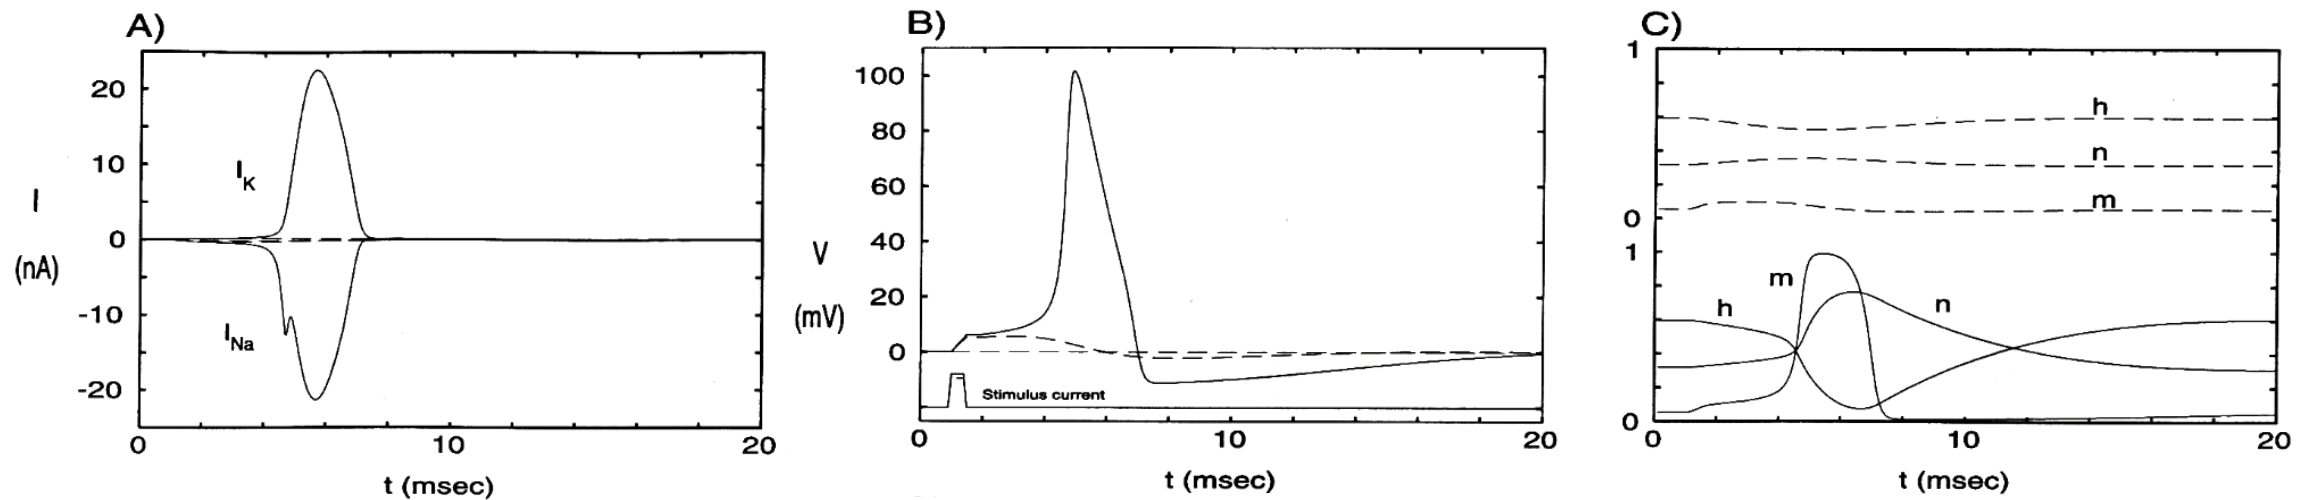
\includegraphics[scale=0.34]{05_5}
    \centering
\end{figure}
To sum up, the HH model is capable to:
\begin{itemize}
    \item Generate action potentials in a correct manner.
    \item Wait for a certain threshold to be overcome in order to initiate a spike.
    \item Exhibit a physiological refractory period after the firing of an action potential.
\end{itemize}
Lastly, it is important to highlight that the kinetics of channels, driven by \(\alpha\) and
\(\beta\) functions, are strongly dependent on temperature as well.

\subsection{Hodgkin-Huxley Model Dynamics}
As show in the picture below, the HH model is capable to fire an action potential
whenever the input stimulus overcomes a certain activation threshold. If this is not
the case, a passive potential - i.e., a partial depolarization - occurs. Note that
the action potential shape produced by this model is highly compatible with the one
observed in experiments.
\begin{figure}[H]
    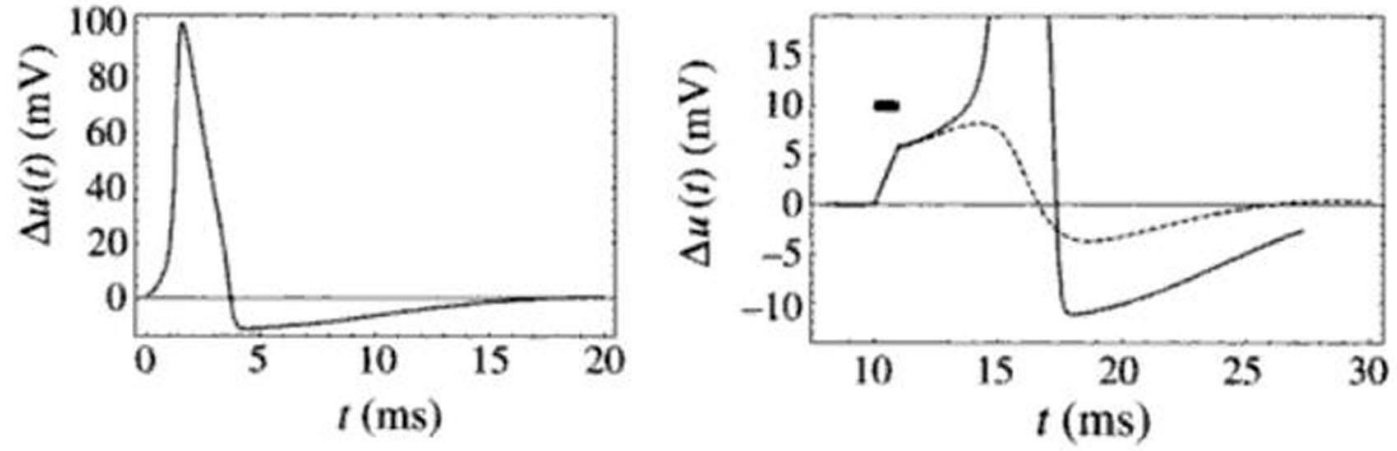
\includegraphics[scale=0.5]{05_6}
    \centering
\end{figure}
If a constant suprathreshold stimulation is provided, then a regular spike train is
observed. The spiking interval is \(T\) and is related to the stimulus amplitude, as
shown by the gain function on the right side. Note that the firing frequency \(f=T^{-1}\)
and it is dependent on the input current (as long as the threhsold is overcome). A minimum
firing rate (\(58\;Hz\)) is present, thus this model cannot fire at lower frequencies.
\begin{figure}[H]
    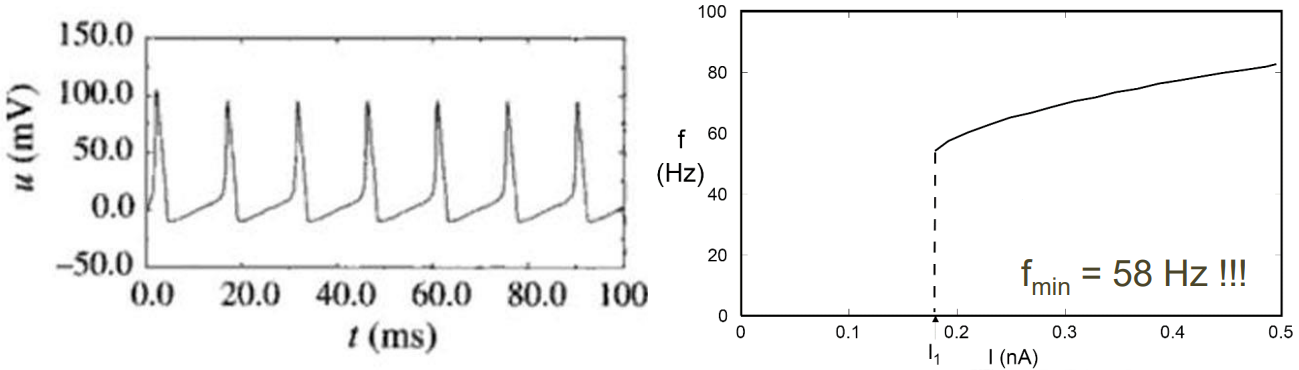
\includegraphics[scale=0.5]{05_7}
    \centering
\end{figure}
Note that if the input current is gradually increased, a higher applied current is needed
to elicit an action potential. In general, a fair current exploits the positive feedback
coming from the fact that Na\({}^{+}\) activating channels (\(m\)) are much faster than the
inactivating ones (\(h\)) and the K\({}^{+}\) activating channels (\(n\)). However, if the
membrane potential is incrementally raised (as the input current increases), the negative
feedback component has time to become stronger. In this condition the neuron is bistable:
\begin{itemize}
    \item Silent if initially quiescent.
    \item Sustained firing if it was already spiking.
\end{itemize}
If the provided stimulation is a step current, the model exhibits different behaviour
according to the size of the step \(\Delta{I}=I_{2}-I_{1}\) and to the final current \(I_{2}\).
\begin{itemize}
    \item Large \(\Delta{I}\Rightarrow\) Spike initiation is facilitated.
    \item Large \(I_{2}\Rightarrow\) Regular firing is more likely to occur.
\end{itemize}
\begin{figure}[H]
    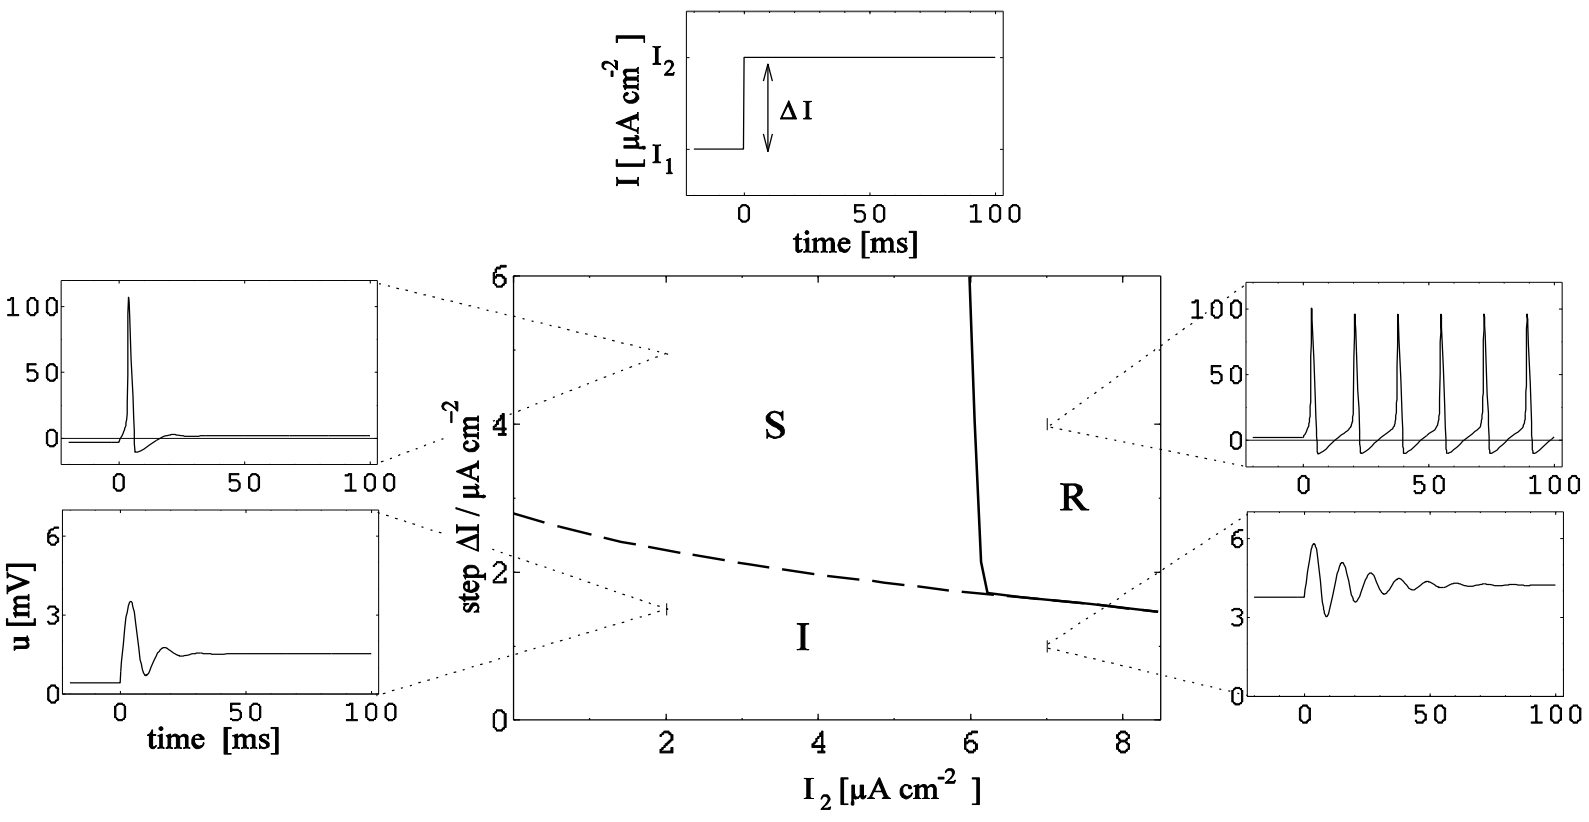
\includegraphics[scale=0.48]{05_8}
    \centering
\end{figure}
In general, the input stimuli can be either external, such as in the case of photoreceptors,
or coming from other close neurons; nonetheless, they are irregular and delivered in a
stochastic way. Typiclly, this means that the response of a neuron should be constituted of
irregular spikes superimposed on a generalized background activity, due to the presence of
noise.
\begin{figure}[H]
    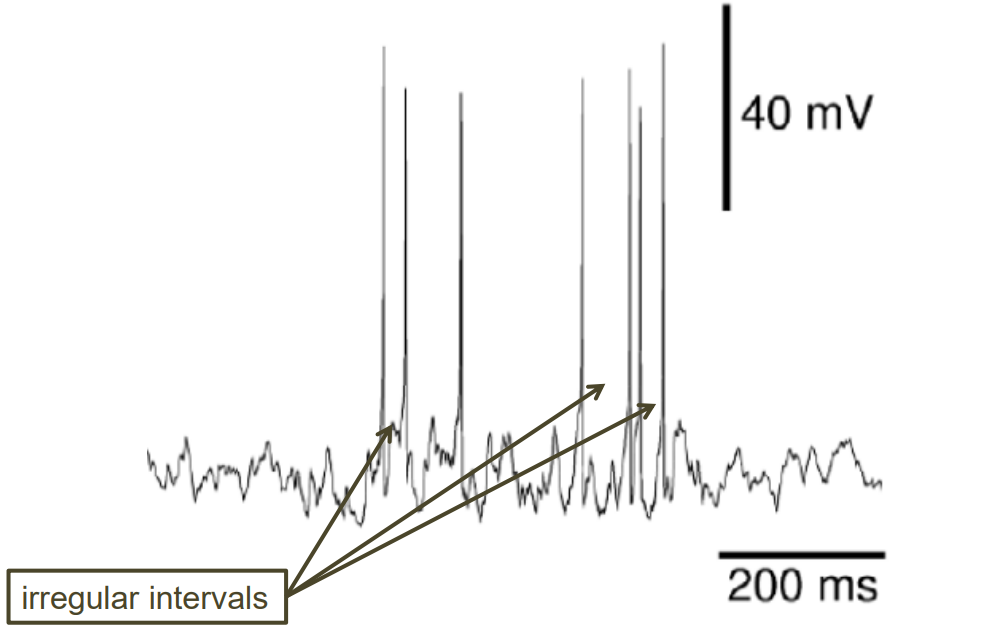
\includegraphics[scale=0.4]{05_9}
    \centering
\end{figure}

\subsection{Hodgkin-Huxley Model Limitations}
Hodgkin divided the neurons in three classes, according to their firing rate characteristics:
\begin{itemize}
    \item \textbf{Class I}: the firing frequency \(f\) can be arbitrarily low, depending on
          the amplitude of the input current. The magnitude of the input is encoded into the
          firing frequency.
    \item \textbf{Class II}: the firing rate is limted to a certain frequency band and it is
          relatively insensitive to changes in the input current magnitude.
    \item \textbf{Class III}: these neurons cannot exhibit sustained spiking activity.
\end{itemize}
The HH model works for Class II neurons, as shown by the gain function.
\begin{figure}[H]
    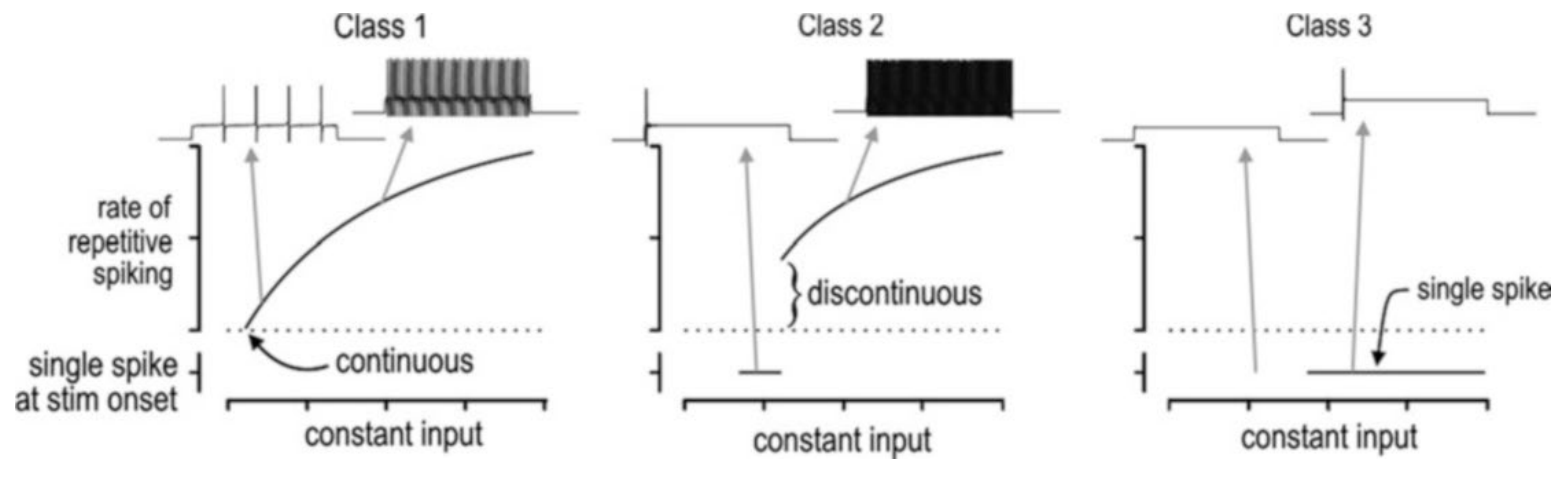
\includegraphics[scale=0.48]{05_10}
    \centering
\end{figure}
Therefore, the HH model does not work if the desired firing rate is low, as regular (tonic)
firing activity is elicited exclusively for high firing frequencies.\\
Another major drawback concerning the HH model is that it cannot reproduce all the
experimentally observed firing patterns. In particular, it is not suitable to model:
\begin{itemize}
    \item Bursting
    \item Adaptation
    \item Post-inhibitory rebound
    \item Resonator
\end{itemize}
Lastly, the HH model is based on the assumption that ion permeation processes are
both continuous and deterministic. Unluckily, this does not hold for very small patches of
cellular membrane, where channels are discrete; in addition, the opening and closing of
channels is ruled by stochastic processes and channels undergo random fluctuations between
open and closed stable states.
\begin{figure}[H]
    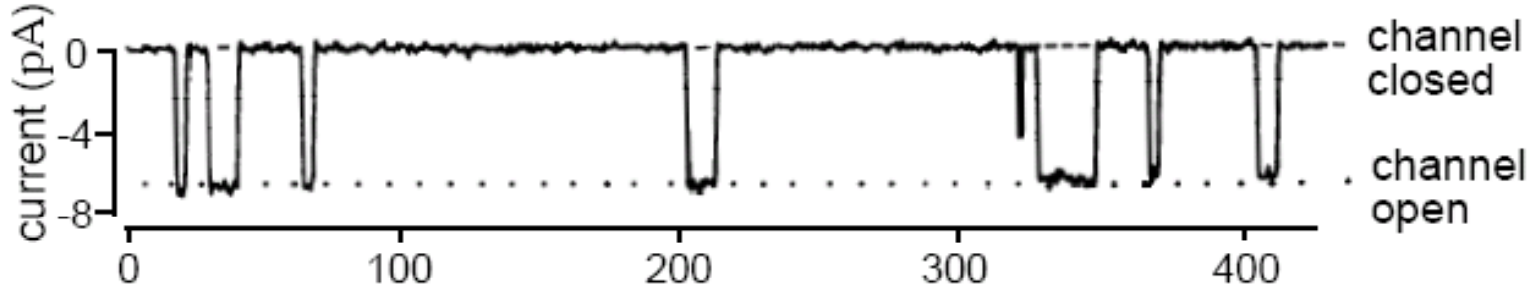
\includegraphics[scale=0.48]{05_11}
    \centering
\end{figure}
\newpage

\section{Multichannel Biophysical Models}
\graphicspath{ {./images/06/} }
As stated in the previous chapter, one of the main limitations displayed by the
Hodgkin-Huxley model is the fact that it can produce only a small fraction of the
activity patterns commonly observed in experiments. Said so, it would be desirable to
build a model able to reproducing virtually all the possible patterns of activity.
\begin{figure}[H]
    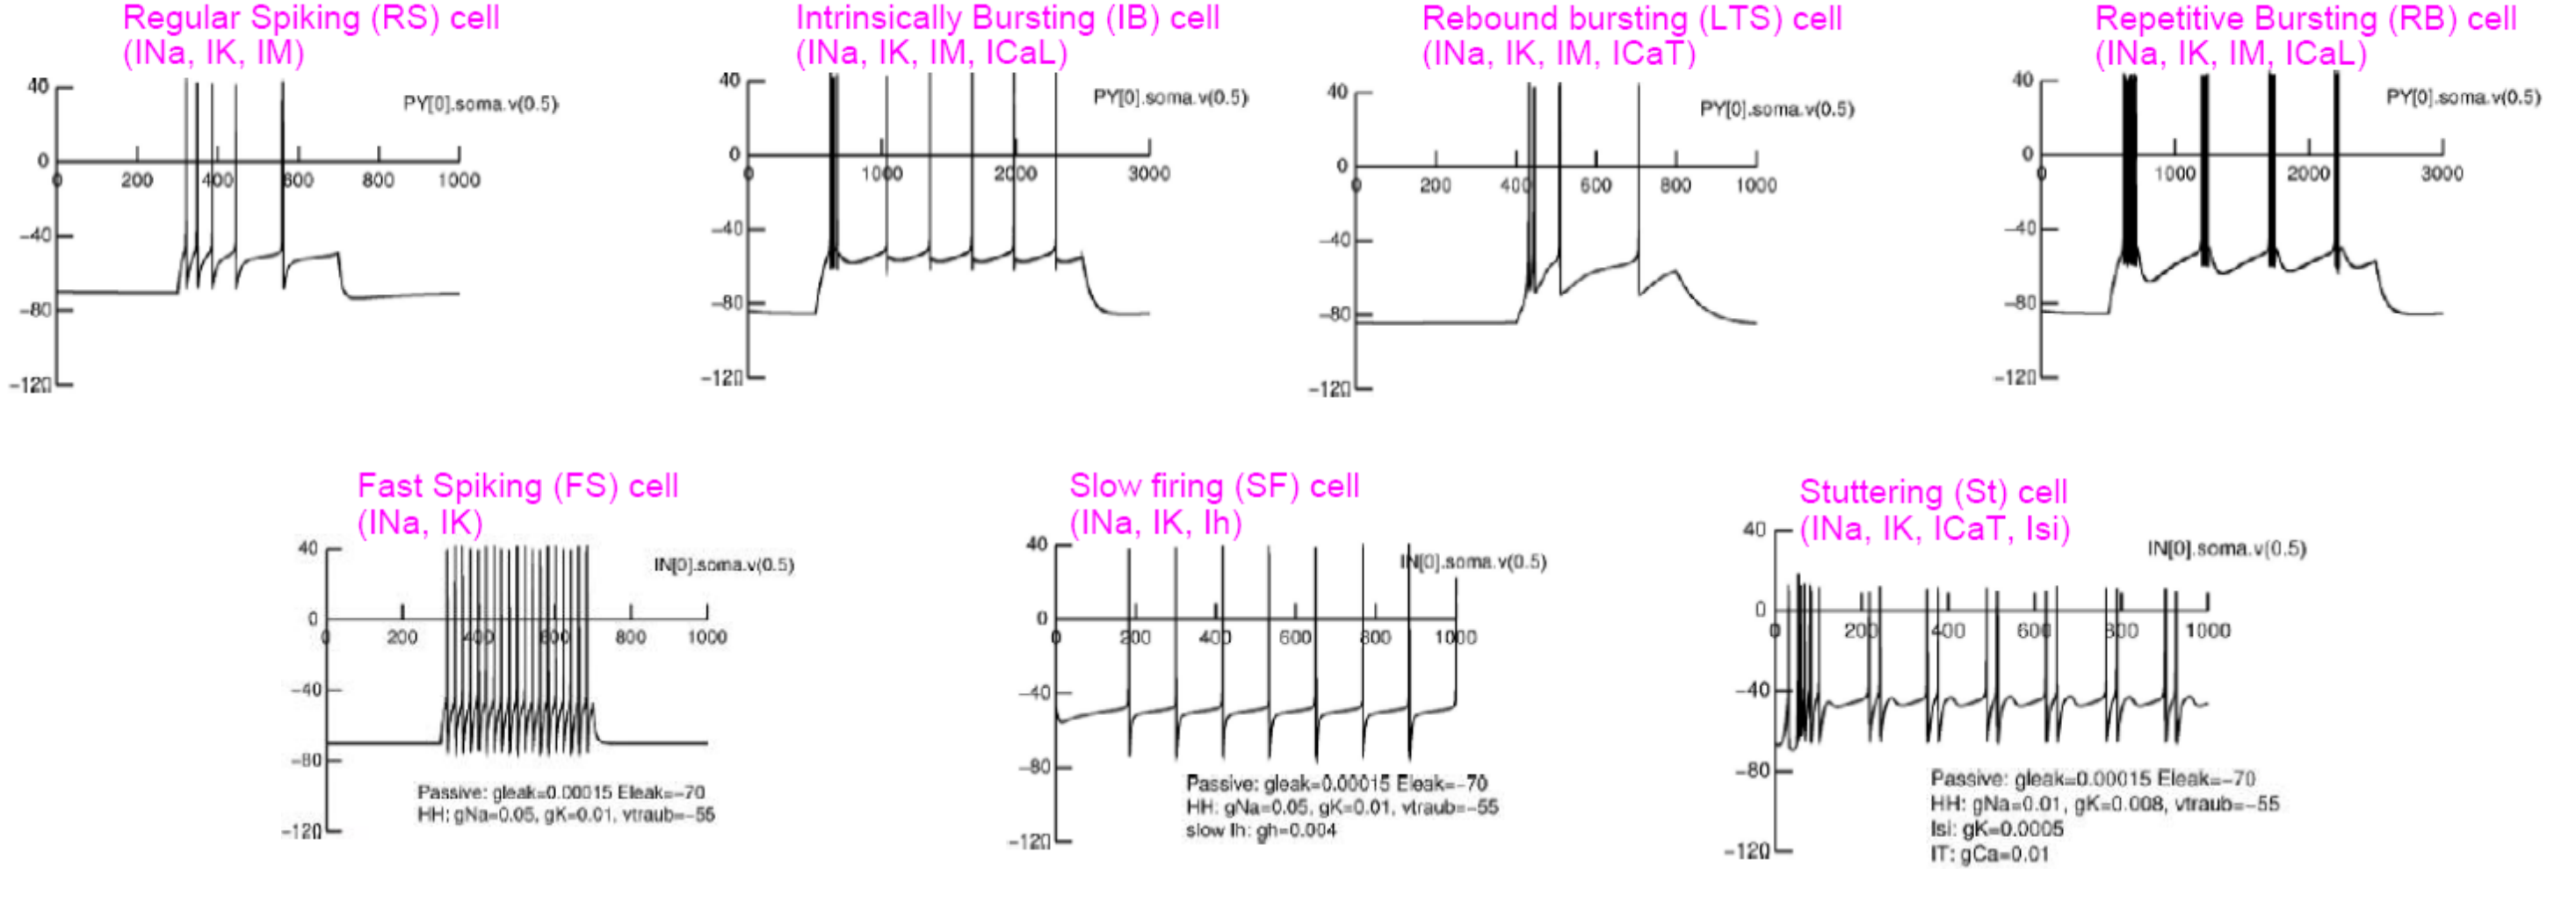
\includegraphics[scale=0.26]{06_1}
    \centering
\end{figure}
Note that these different patterns are a consequence of different ionic channels being
involved, each one with a different kinetics.
\begin{itemize}
    \item \textbf{Inward currents}: sodium current (fast), sodium current (persistent),
          calcium current (low-threshold), calcium current (high-threshold).
    \item \textbf{Outward currents}: potassium current (several families of channels).
\end{itemize}
A generic ionic current for the ions of type \(j\) can be formalized as follow:
\begin{equation*}
    I_{j}=\bar{g}_{j}\cdot{m^{p_{j}}h^{q_{j}}}\cdot{(V_{m}-E_{j})}
\end{equation*}
where the \(m\) gating particle is activating and \(h\) inactivating.

\subsection{Channels Types}
\subsubsection{Sodium Channels}
\paragraph{Fast Sodium Channels (\(I_{Na}\))} This is the kind of sodium chnnels
considered in the HH model, described by
\begin{equation*}
    I_{Na}=\bar{g}_{Na}\cdot{m^{3}h}\cdot{(V_{m}-E_{Na})}
\end{equation*}
\paragraph{Persistent Sodium Channels (\(I_{NaP}\))} This type of channel has \(q_{NaP}=0\),
therefore it is described by
\begin{equation*}
    I_{NaP}=\bar{g}_{NaP}\cdot{m}\cdot{(V_{m}-E_{Na})}
\end{equation*}
Note that if a neuron with only persistent sodium channels is considered, it would
constantly depolarize.\\
In addition to this consideration, the time constants of sodium gating particles are
comparable, thus sodium channels are responsible for hyperpolarization and depolarization,
but they are not able to produce spikes on their own.
\subsubsection{Potassium Channels}
\paragraph{Rapidly Inactivating Potassium Channels (\(I_{A}\))} They present two distinct
subtypes and have a time constant \(\tau_{h}\approx{10\;ms}\).
\paragraph{Slowly Inactivating Potassium Channels (\(I_{K}\))} They present two distinct
subtypes and have a time constant \(\tau_{h}\approx{200\;ms}\).\\
Note that the time constant of potassium \(\tau_{h,A}>>\tau_{h,Na}\), therefore the ionic
current \(I_{A}\) tends to hyperpolarize the membrane potential, slowing down the firing
rate: new action potentials occur as soon as the \(I_{A}\) current has become sufficiently
inactivated. Hence, the HH model in conjunction with these families of potassium channels
is able to model \textbf{Type I} neurons, even with very low firing frequencies, as
visible in the plot below.
\begin{figure}[H]
    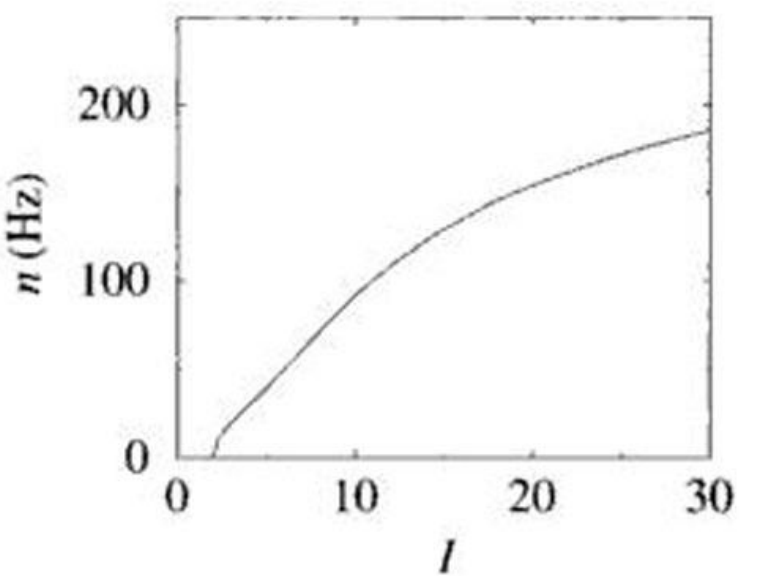
\includegraphics[scale=0.35]{06_2}
    \centering
\end{figure}
\subsubsection{Calcium Channels}
Differently from Na\({}^{+}\) and K\({}^{+}\), the concentration of Ca\({}^{2+}\) ions
is extremely low inside a cell and it is significantly affected by the calcium influx
occuring during an action potential. In particular, calcium has two functions in the
generation of an action potential:
\begin{itemize}
    \item Carry a positive electrical charge, contributing to depolarization.
    \item Modulate the activity of other channels, being a second messenger.
\end{itemize}
\paragraph{Low-Threshold Calcium Channels (\(I_{T}\))} These are inactivating channels,
similar to \(I_{Na}\), but differring in the shifting of the activation and inactivation
curves towards a hyperpolarized membrane potential: these channels are completely
inactivated at resting potential. In this case, an action potential can be elicited
by an inhibitory (hyperpolarizing) input, as a matter of fact, when it is switched off,
an overshoot of the action potential is observed, due to a quick depolarization of the
membrane, generating a low-threshold calcium spike: this phenomenon is known as
post-inhibitory rebound.
\begin{figure}[H]
    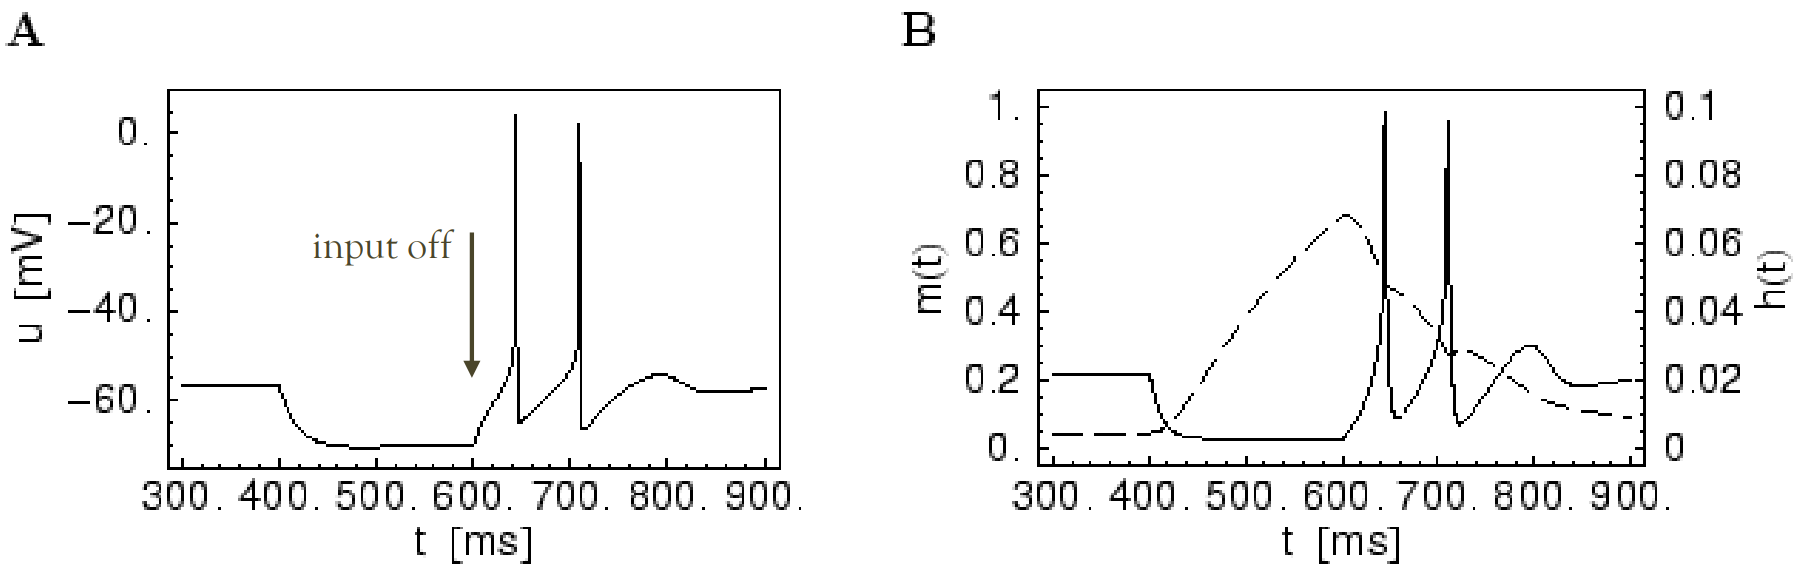
\includegraphics[scale=0.28]{06_3}
    \centering
\end{figure}
\paragraph{High-Threshold Calcium Channels (\(I_{L}\))} These channels produce a
non-inactivating current, which can be activated only at high levels of depolarization.
For instance, this current is responsible for the generation of bursting patterns.
\begin{equation*}
    I_{L}=\bar{g}_{Ca}\cdot{m^{2}}\cdot{(V_{m}-E_{Ca})}
\end{equation*}
\subsubsection{Calcium-Activated Potassium Channels}
There are two main families of calcium-activated potassium channels:
\begin{itemize}
    \item \textbf{\(I_{C}\)}: these channels depends on both voltage and Ca\({}^{2+}\)
          concentration.
          \begin{equation*}
              I_{C}=\bar{g}_{C}\cdot{m}\cdot{(V_{m}-E_{K})}
          \end{equation*}
    \item \textbf{\(I_{AHP}\)}: these channels are slower than the \(I_{C}\) ones and they
          depend solely on Ca\({}^{2+}\) concentration.
          \begin{equation*}
              I_{AHP}=\bar{g}_{AHP}\cdot{m}\cdot{(V-E_{K})}
          \end{equation*}
          Note that \(I_{AHP}\) is a non-inactivating current and due to the low time constant,
          each spike increases the activation of the gating particle \(m\). If the neuron is
          stimulated by a constant depolarizing current, each action potential elicited increases
          the amount of open AHP channels, therefore the corresponding  \(I_{K}\) is
          subtracted from the applied stimulus. This causes a decrease in the firing frequency:
          such a phenomenon is called adaptation.
          \begin{figure}[H]
              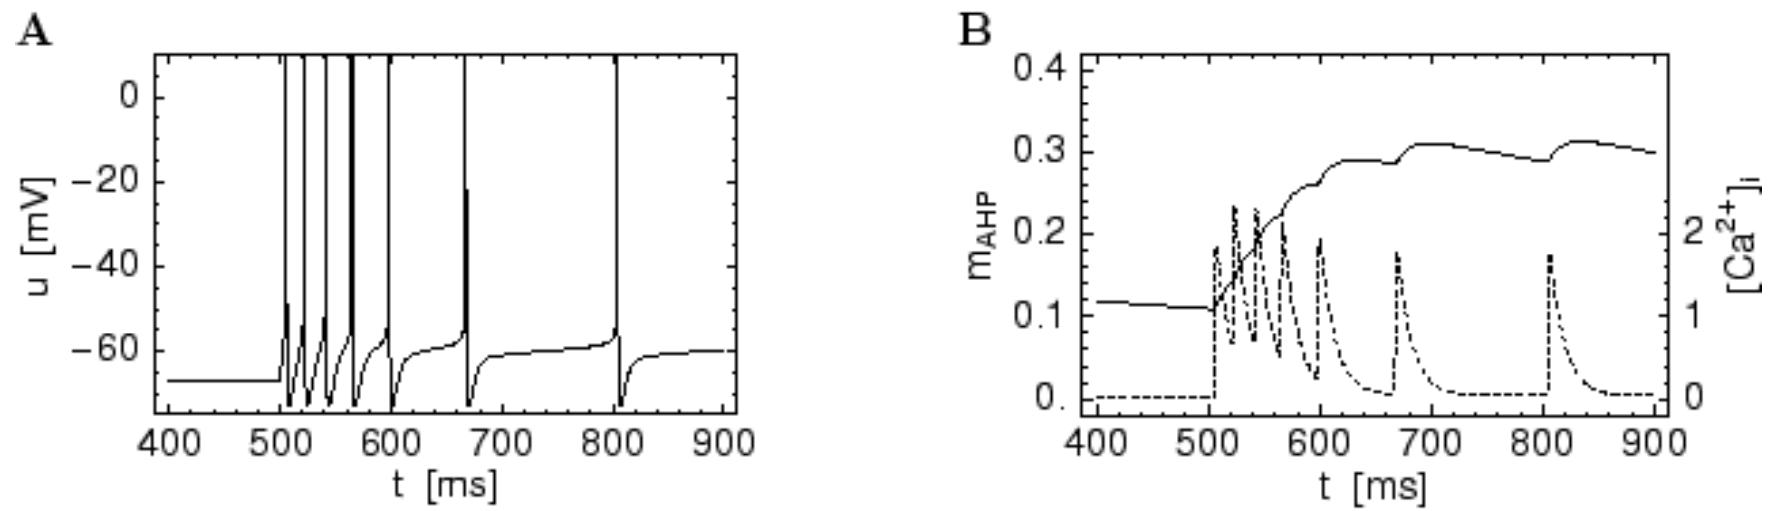
\includegraphics[scale=0.28]{06_4}
              \centering
          \end{figure}
\end{itemize}
Finally, the differential equation describing the model of a neuron (compartment \(k\))
can be as:
\begin{equation*}
    C_{k}\frac{dV_{k}}{dt}=\sum_{j}g_{j,k}(V_{j}-E_{k})-I_{ionic,k}
\end{equation*}
The ionic channels to consider are distributed as follow:
\begin{itemize}
    \item Na\({}^{+}\) channels: 2
    \item Leakage channels: 1
    \item K\({}^{+}\) channels: 6
    \item Ca\({}^{2+}\) channels: 2
\end{itemize}

\subsection{Stimulation and Activity Patterns}
Note that when stimulating a neuron it is important to carefully select the stimulation
amplitude and the location where it is delivered, as they both affect the neuron response.
\begin{figure}[H]
    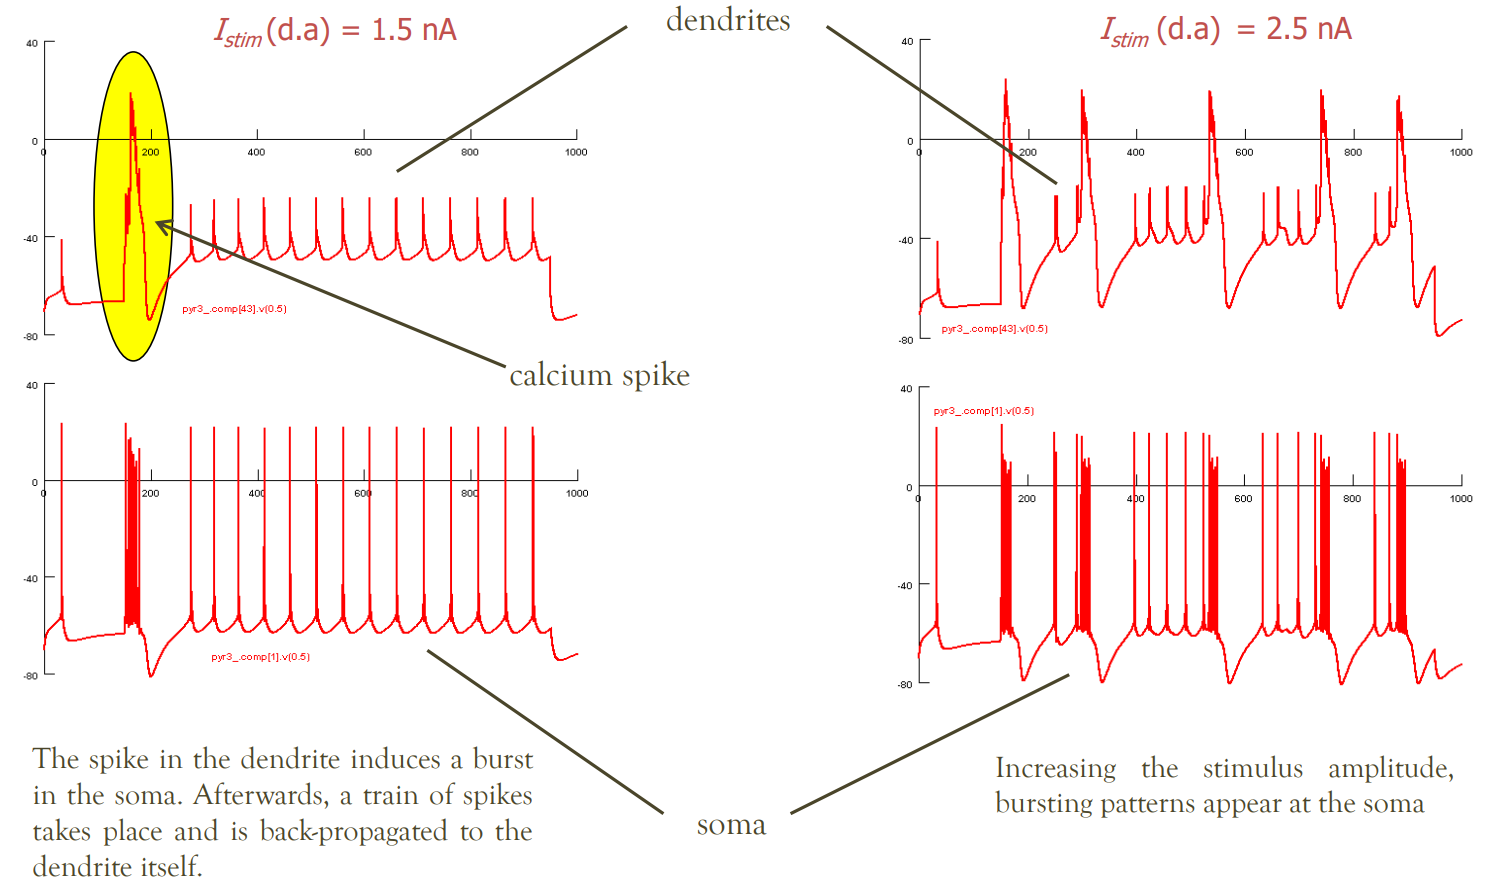
\includegraphics[scale=0.4]{06_5}
    \centering
\end{figure}
Apart from typical spikes, other kinds of activation might be observed:
\begin{itemize}
    \item \textbf{Spikelets}: small action potentials with an amplitude below \(10\;mV\).
    \item \textbf{Partial Spikes}: action potentials with an amplitude ranging from \(10\)
          to \(25\;mV\).
\end{itemize}
\begin{figure}[H]
    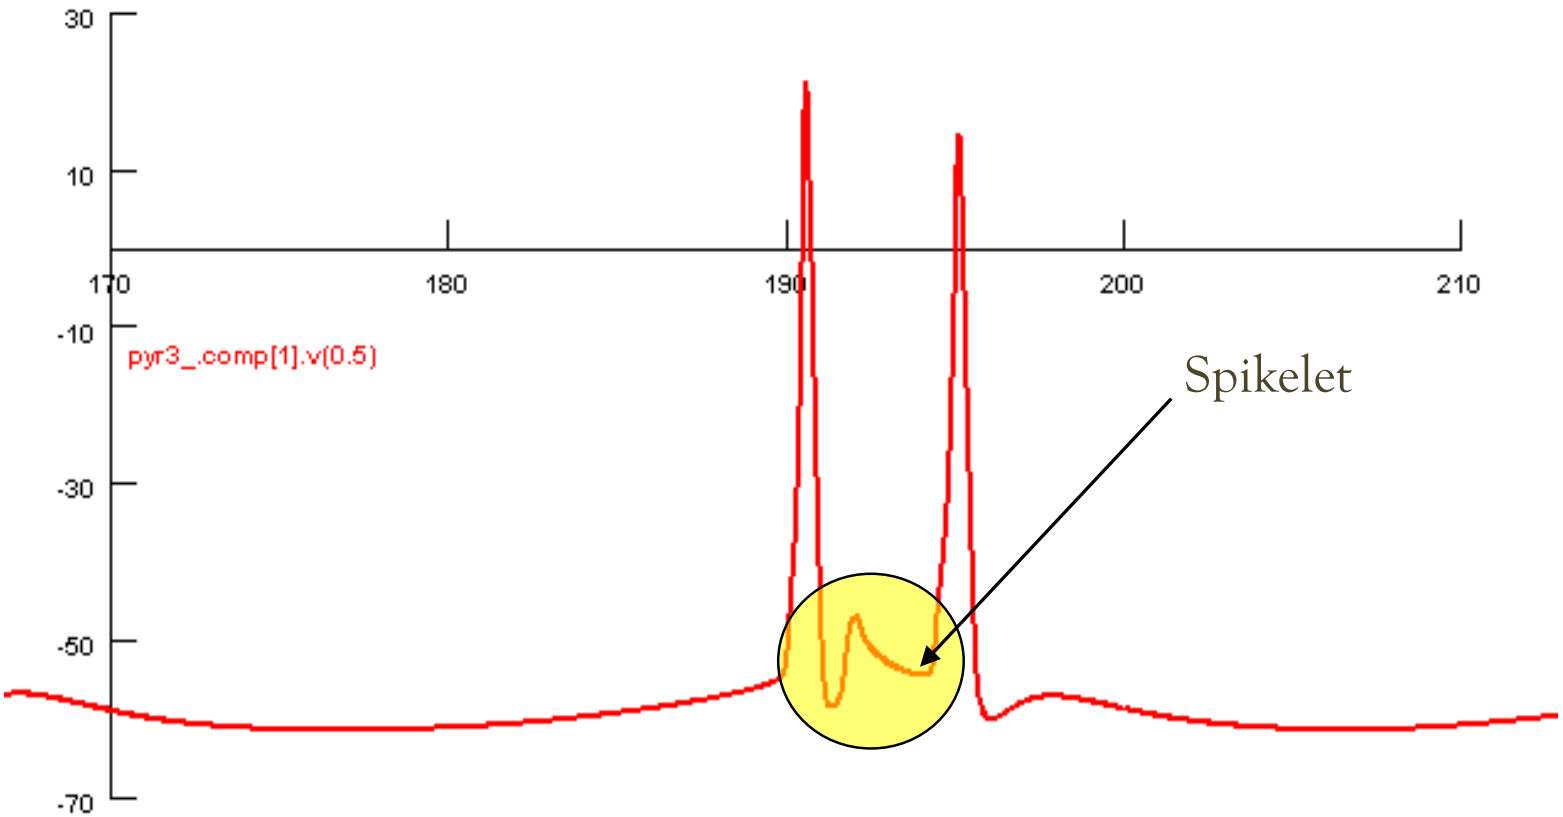
\includegraphics[scale=0.24]{06_6}
    \centering
\end{figure}
Also bursts are not all identical, but they might present different features according to
the stimulation site.
\paragraph{Apical Dendrites} A stimulation there may evoke both small spikes (due to fast
Na\({}^{+}\) channels) and spike trains separated by action potentials due to the
slow high-threshold Ca\({}^{2+}\) channels kinetics.
\paragraph{Soma} In the soma there are no calcium channels, as they exist only in the
dendrites. A more rythmic activity is thus induced, in addition the stimulation amplitude
highly shapes the response. Note that persistent Na\({}^{+}\) channels play a crucial role
in switching from rythmic spiking to rythmic bursting in the soma.
\newpage

\section{Stochastic Neuronal Models}
\graphicspath{ {./images/07/} }
As pointed out in the previous pages, the Hodgkin-Huxley model presents a number of
limitations, in particular it is based on the hypothesis that the membrane ion
permeation processes are continuous and deterministic. Unluckily this is not the case,
as a matter of fact spontaneous currents pass through voltage-dependent sodium channels,
causing a noisy and spontaneous activity of the neuron. As a consequence, stochastic models
are necessary to better describe the random fluctuations of discrete ion channels between
open and closed states.

\subsection{Multistate Channels}
It has been shown that the transmembrane ionic channels present complex molecules involving
several states and transitions: there are not only open and closed states, but also a
lot of intermediate situations.\\
If the number of gates is \(k=3\), it means that there are \(2^{k}=2^{3}=8\) different states,
among which only one represents the full open configuration, allowing the ions to flow
through the membrane.
\begin{figure}[H]
    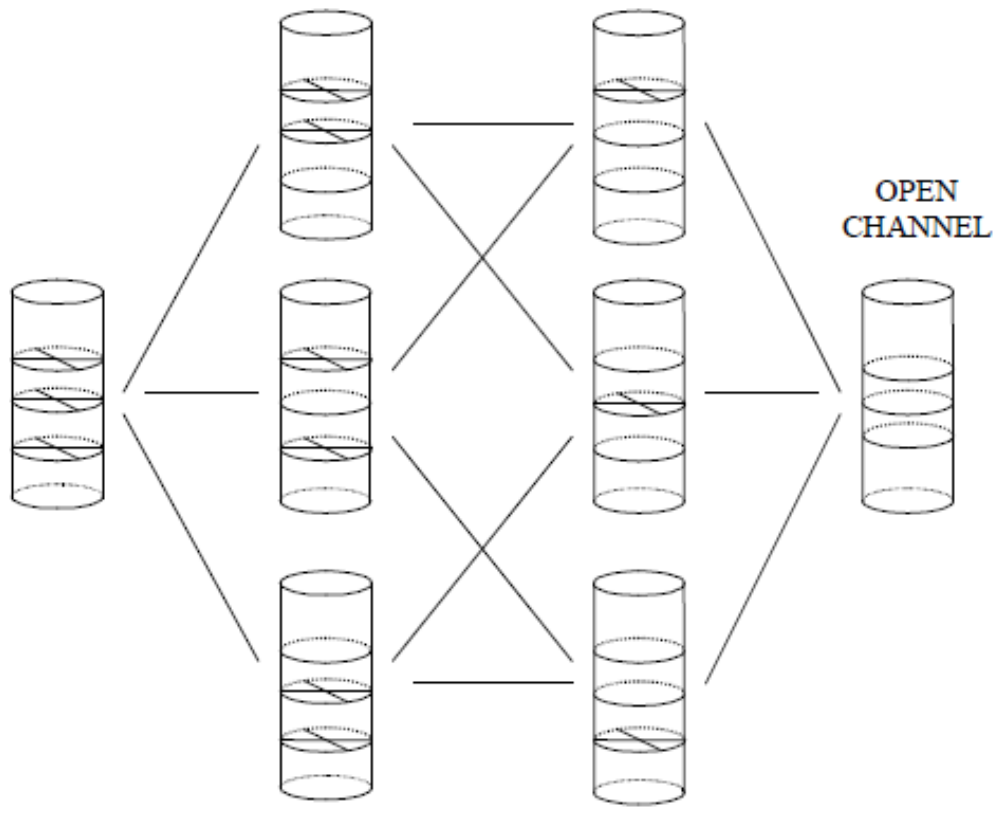
\includegraphics[scale=0.42]{07_1}
    \centering
\end{figure}
The binary activation of a certain channel with \(k\) gates is then defined as
\begin{equation*}
    \xi=\prod_{j=1}^{k}\gamma_{j}
\end{equation*}
where \(\gamma_{j}\) is the binary activation variable for the \(j\)-th gate. Note that
\(\gamma_{j}=1\) if the corresponding \(j\)-th gate is open and, consequently, \(\xi=1\)
only if all the \(k\) gates are open at the same time, otherwise \(\xi=0\).\\
To model the possible \(2^{k}\) states of a channel and the transitions among such states,
a Markov model can be employed. If the states are a finite number (\(2^{k}\)), then also the
transitions are finite.\newpage
Some assumptions are thus necessary:
\begin{itemize}
    \item The states of a single ionic channel are separated by large energy barriers. When the
          channel reaches the right amount of energy, a transition occurs.
    \item The probability to perform a transition depends only on the currently occupied state.
    \item The previous history of occupied channels is not relevant, only the membrane voltage elicits
          a transition, overcoming the energy barrier.
    \item The duration for which the present state remained occupied is not relevant.
\end{itemize}
Henceforth, the time evolution of the probability to occupy state \(S_{i}\) is described by the
equation
\begin{equation*}
    \frac{dP(S_{i},t)}{dt}
    =\sum_{j=1}^{n}P(S_{j},t)P(S_{j}\rightarrow{S_{i}})-\sum_{i=1}^{n}P(S_{i},t)P(S_{i}\rightarrow{S_{j}})
\end{equation*}
where \(P(S_{i},t)\) is the probability of being in state \(S_{i}\) at time \(t\) and
\(P(S_{i}\rightarrow{S_{j}})\) is the probability to have a transition from state \(S_{i}\)
to state \(S_{j}\). Note that, generally speaking, transitions are reversible.\\
If a large number of identical channels is considered, the probability of being in a state \(S_{i}\) can
be reinterpreted as the fraction of channels occupying the \(S_{i}\) state, denoted by \(s_{i}\), while
the transition probability \(P(S_{i}\rightarrow{S_{j}})\) becomes the rate constant of the reaction, \(r_{ij}\).
As a consequence, the previous equation can be rewritten in these terms:
\begin{equation*}
    \frac{ds_{i}}{dt}=\sum_{j=1}^{n}s_{j}r_{ji}-\sum_{i=1}^{n}s_{i}r_{ij}
\end{equation*}
Said so, the HH model should be modified according to the stochastic processes described above:
\begin{gather*}
    C_{m}\frac{dV}{dt}
    =\bar{g}_{Na}\cdot{m^{3}h}\cdot{(V_{m}-E_{Na})}
    +\bar{g}_{K}\cdot{n^{4}}\cdot{(V_{m}-E_{K})}
    +g_{leak}\cdot{(V_{m}-E_{leak})}\\
    \Downarrow\\
    C_{m}\frac{dV}{dt}
    =\bar{g}_{Na}\cdot{m}\cdot{(V_{m}-E_{Na})}
    +\bar{g}_{K}\cdot{n}\cdot{(V_{m}-E_{K})}
    +g_{leak}\cdot{(V_{m}-E_{leak})}
\end{gather*}
where \(m\) and \(n\) are stochastic processes of time and represent the fraction of open channels
selective to Na\({}^{+}\) and K\({}^{+}\) ions respectively.\\
By assuming \(N_{Na,max}\) and \(N_{K,max}\) the total number of sodium and potassium channels
respectively, it can be stated that:
\begin{gather*}
    m=\frac{1}{N_{Na,max}}\sum_{i=1}^{N_{Na,max}}\xi_{Na,i}\\
    n=\frac{1}{N_{K,max}}\sum_{i=1}^{N_{K,max}}\xi_{K,i}
\end{gather*}
Note that the binary activations reported here are to be derived by the binary activation variables,
identifies, described, and modelled through patch-clamp measurements of single channels.\\
An example of a model for potassium channels is shown here, note how the channel has to go through all
the intermediate states in order to reach the open configuration.
\begin{figure}[H]
    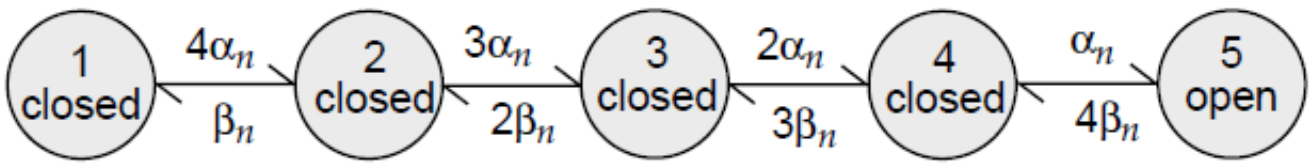
\includegraphics[scale=0.3]{07_2}
    \centering
\end{figure}
Concerning sodium channels, the HH model assumes activation and inactivation processes to be independent,
however that is not the case, as they are interdependent. In particular:
\begin{itemize}
    \item The activation process is voltage-dependent.
    \item The inactivation process is state-dependent (and voltage-independent).
\end{itemize}
Thus, an exaple model for the sodium channels can be the following one:
\begin{figure}[H]
    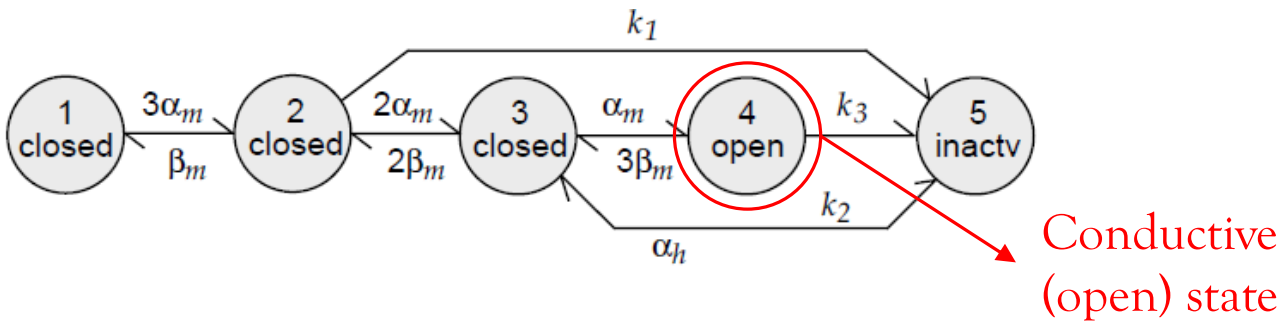
\includegraphics[scale=0.38]{07_3}
    \centering
\end{figure}
The inactive state displayed on the right side means that the channel stops depolarizing, exhibiting
a sort of refractory period, as it is not able to open again and allow the passage of ions.\\
By employing these stochastic models, the behaviour of a single channel is very far from the one
observed through the Hodgkin-Huxley model; nonetheless, by increasing the number of considered
channels the dynamics tend to be coincident with the HH model one. Therefore, it can be said
that stochastic models tends to be equivalent to the HH model as long as a large number of
channels is observed.
\begin{figure}[H]
    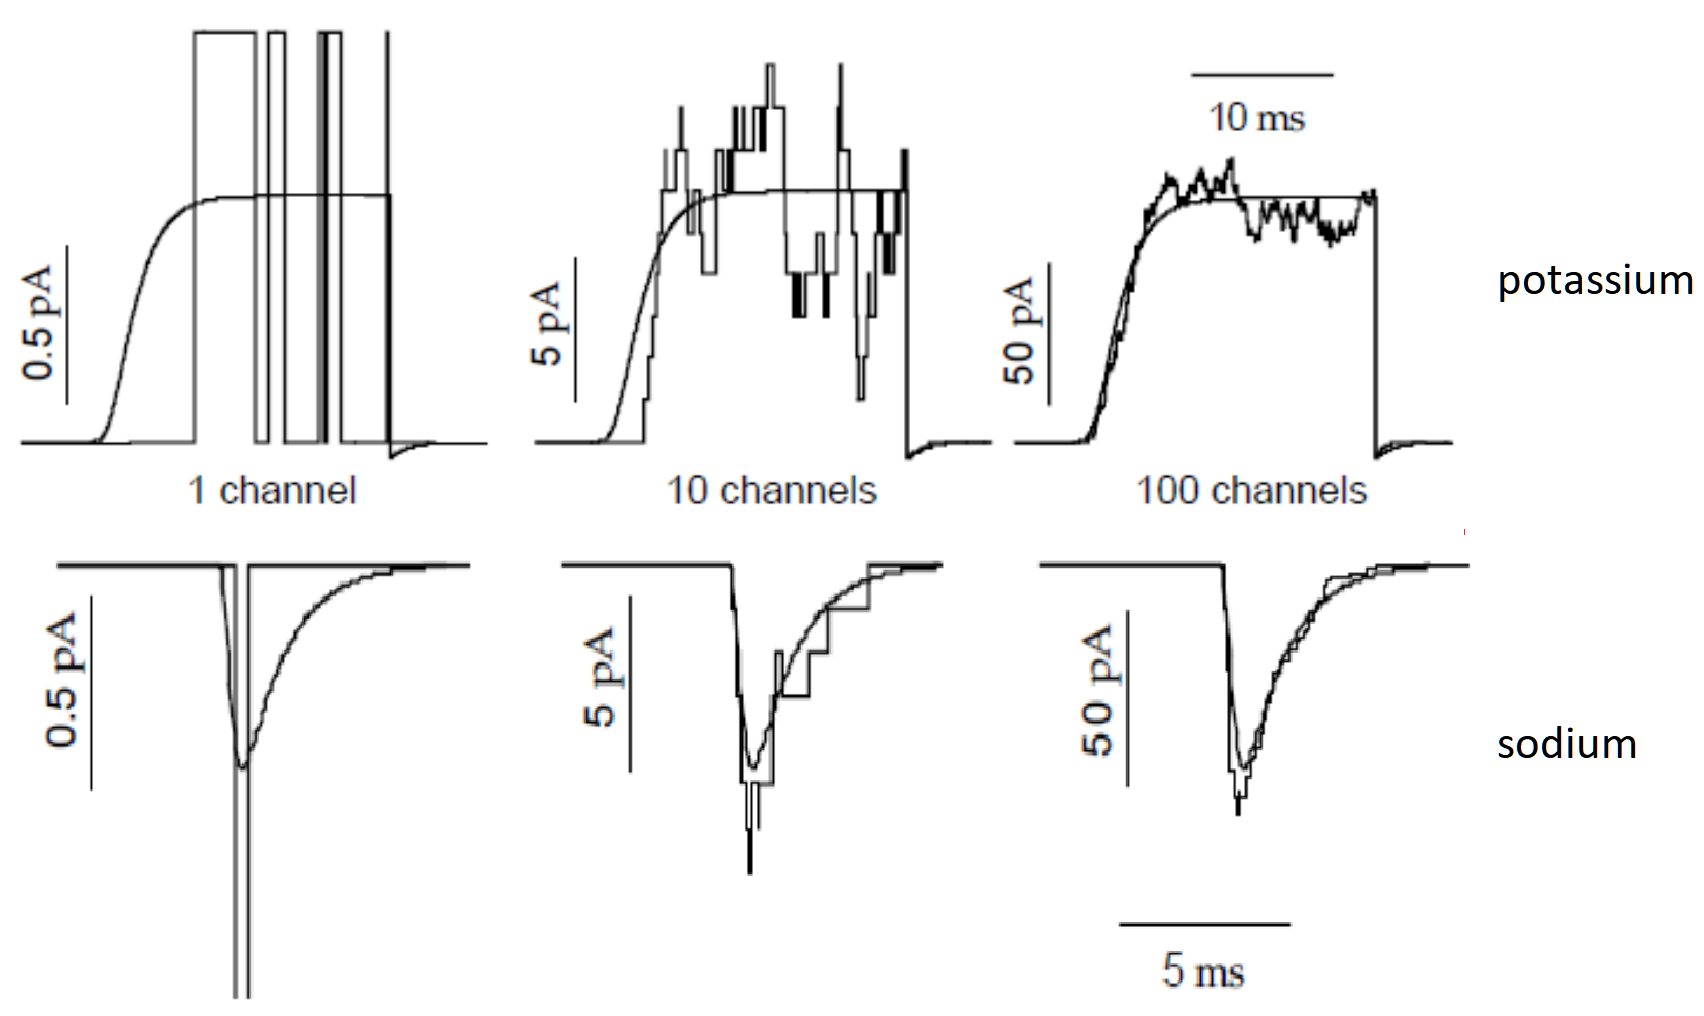
\includegraphics[scale=0.3]{07_4}
    \centering
\end{figure}
\paragraph{Why different models (HH and stochastic ones) display similar behaviours?} This is a
consequence of the speed of the activation process for the Na\({}^{+}\) conductance. In particular,
the activation variable \(m\) of the HH model reaches its voltage-dependent steady-state value
\(m_{\infty}(V_{m})\) extremely rapidly (\(\tau_{m}\approx{1\;ms}\)), making it difficult to distinguish
inactivation processes dependending on \(m\) from those depending on \(V_{m}\).
\begin{figure}[H]
    \includegraphics[scale=0.45]{07_5}
    \centering
\end{figure}
Also in the plots above it can be seen that increasing the number of observed channels leads to
a model similar to the HH one. This is true also in the case of current stimulations, as depicted below.
\begin{figure}[H]
    \includegraphics[scale=0.45]{07_6}
    \centering
\end{figure}
Note that the voltage is shown for different amounts of channels as a function of time. With no stimulation,
a flat potential is expected, precisely at the resting potential \(E_{r}\), however if small groups
of channels are considered (a small patch of cell membrane), there are several random fluctuations which
are not able to cancel each other out, resulting in a noisy activity. Similar considerations are true also
in the case where a DC stimulation is present.

\subsection{Voltage-Gated Sodium Channels}
In humans there are nine isomers of voltage-gated sodium channels (VGSC), each one with peculiar kinetics
and tissue distribution. Note that even slight changes of their gating kinetics may cause severe diseases.\\
Ideally, it is deasirable to model these sodium channel isomers through the Markov approach, employing the
possible lowest number of states, as the computational cost should be as light as possible. At the moment,
the model employing the fewest states is the Balbi one, with six states.
\begin{figure}[H]
    \includegraphics[scale=0.35]{07_7}
    \centering
\end{figure}
The Balbi model is arranged in two closed, two open, and two inactivated states. All transitions are
reversible but one.\\
When developing such a model, one of the most time-consuming and critical steps is the model
parameters tuning, which aims at matching the experimental data.
\newpage

\section{Noise in Neuronal Structures}
\graphicspath{ {./images/08/} }
A complex system is generally characterized by variability and neurons make no
exception. In this setting, variability refers to changes in some measurable quantities,
such as the spike timing. The main type of variability is the trial-to-trial one, which
can be observed across repetitions of the same experiment.
\begin{figure}[H]
    \includegraphics[scale=0.3]{08_1}
    \centering
\end{figure}
The sources of trial-to-trial variability are mainly two:
\begin{enumerate}
    \item \textbf{Deterministic properties of the system}: the initial state of the
          neuronal circuit might not be always the same.
    \item \textbf{Noise}: it is defined as random or unpredictable fluctuations
          and disturbances not belonging to the signal, which can be addictive or distort
          the signal. Noise is a crucial issue in information processing.
\end{enumerate}
Noise can be categorized into several types according to its statistical properties.
A partial solution might consist in filtering out some of the noise; on the other hand,
it might be important to investigate how and where such noise is originated.\\
The main sources of noise in the nervous system are reported in this schema.
\begin{figure}[H]
    \includegraphics[scale=0.32]{08_2}
    \centering
\end{figure}
\paragraph{Sensory Noise} External sensory stimuli are intrinsically noisy. In particular,
they are converted from several distinct domains, such as the electromagnetic one in the
case of photoreceptors, into chemical or mechanical signals. Then, such signal is amplified
and converted into an electrical one. In addition, it has been observed that stimulating
neurons with a constant stimulus, for instance a DC current, is all but natural, as real world
stimuli are far from being constant and steady; on the contrary, a natural stimulus does not
provide constant features, thus the nervous system is used to deal with noisy inputs and
extract useful information from them.
\paragraph{Cellular Noise} If neurons are driven with identical constant stimuli over repeated
trials, the timing of the elicited action potentials varies across the trials. Such a variability
is in the order of \(ms\), or even lower, but it drastically affects the capability of neurons
to detect coincident signals or their order of arrival.\\
Note that the neuronal activity might look random without actually being random. Even if the
statistical characteristics of neuronal variability resemble the ones typical of a random process,
it does not necessarily mean that the firing pattern observed is generated by such a random process.
Shannon's theory of information states that when the optimal encoding is used to maximize information
transmission, the signal will look random.

\subsection{Sources of Cellular Noise}
\paragraph{Electrical Noise} This kind of noise causes membrane potential fluctuations, either with
or without synaptic inputs. Most of the electrical noise in a cell is channels noise, which is
made of electrical currents produced by the random opening and closing of ion channels.\\
Note that if \(N\) channels are considered, the coefficient of variation \(CV\) is computed
as follow:
\begin{equation*}
    CV=\sqrt{\frac{variance}{mean}}=\sqrt{\frac{1-p(V)}{N\cdot{p(V)}}}
\end{equation*}
Therefore, it can be stated that \(CV\propto{\frac{1}{\sqrt{N}}}\), hence the noisiness of a membrane current
declines proportionally to the square root of the number of channels \(N\).
\begin{figure}[H]
    \includegraphics[scale=0.275]{08_3}
    \centering
\end{figure}
As already observed, if \(N\) is small, then the variability of a single channel is very high, but if a large
set of channels is taken into account, the model tends to be compliant with the Hodgkin-Huxley model, which
is deterministic and does not take into account noise.
\paragraph{Johnson Noise} It is related to the temperature and is generated by the thermal agitation of charge
carriers inside an electrical conductor. It is dependent on the material considered.
\paragraph{Shot Noise} This is a type of noise whenever the amount of signal particles (such as electrons or ions
in an electrical circuit or photons hitting a photoreceptor) is small enough to give rise to detectable
statistical fluctuations in a measurement, not enabling a correct and reliable esteem of the incoming
information.
\paragraph{Synaptic Noise} Synapses are always releasing a certain quantity of neurotransmitters
(synaptic bombardment), some of them might evoke some kind of response in the post-synaptic terminal
(spontaneous miniature post-synaptic current or mPSC) even if no
action potential was fired. This kind of noise is diffuclt to address, as multiple sources are involved.
In addition, the relevance of this phenomenon is greater in highly connected neurons, as the integration
effect of neurotransmitters coming from all of the available synapses is no longer negligible.

\subsection{Reliability and Noise}
Despite the brain noise, it has been shown that such noise plays a fundamental role in neural
information processing. It enhances the reliability and regularity of neuronal firing both
in single neurons and populations. Researchers demonstrated that a constant DC stimulation
generated firing patterns with a considerable variability across trials, while if random
noisy fluctuations are superimposed on such a stimulus, then the reliability of spikes
is enormously improved. This can be explained by saying that natural inputs are in fact noisy
and the nervous system is therefore designed to work with them.
\begin{figure}[H]
    \includegraphics[scale=0.24]{08_4}
    \centering
\end{figure}
Neurons fire in a clock-like fashion, with spikes being separated by fixed time intervals.
Noise facilitates this spiking periodicity.
\begin{itemize}
    \item \textbf{Stochastic Resonance}: if a neuron receives a sub-threshold time-varying input,
          then the addition of noise induces action potentials only during the peaks of such signal,
          when the activation threshold is overcome.
    \item \textbf{Coherence Resonance}: in this case neurons receive exclusively noise with a
          supra-threshold amplitude. The response is thus more synchronized, with \(CV\to{0}\).
\end{itemize}
To sum up, it should be highlighted that noise is crucial when dealing with neurons. Hence,
when building a model (at any scale) it is vital to properly take into account noisy
components. This is particularly true when the investigated topic is the coding capability of
a neuron, as coding cannot neglect the effect of spontaneous fluctuations.
\newpage

\section{Reduced Biophysical Models}
\graphicspath{ {./images/09/} }
Let's now recall for a moment the Hodgkin-Huxley model:
\begin{equation*}
    C\frac{dV}{dt}=-\bar{g}_{Na}m^{3}h(V-E_{Na})-\bar{g}_{K}n^{4}(V-E_{K})-g_{leak}(V-E_{leak})+I_{app}
\end{equation*}
The dynamics of the gating particles is reported here and depicted below:
\begin{align*}
    \frac{dm}{dt} & =\alpha_{m}(V)(1-m)-\beta_{m}(V)m \\
    \frac{dh}{dt} & =\alpha_{h}(V)(1-h)-\beta_{h}(V)h \\
    \frac{dn}{dt} & =\alpha_{n}(V)(1-n)-\beta_{n}(V)n
\end{align*}
\begin{figure}[H]
    \includegraphics[scale=0.25]{09_1}
    \centering
\end{figure}
The goal now is to switch from a model described by four differential equations (as the HH one), to
a model with reduced complexity, described only by two equations. Henceforth, some simplifications
are to be done:
\begin{enumerate}
    \item The \(\tau_{m}\) time constant, related to the gating particle \(m\), is extremely small if
          compared to \(\tau_{h}\) and \(\tau_{n}\), implying an almost instantaneous depolarization. Therefore,
          it can be said that the action potential peak due to \(m\) occurs immediately and that \(m\) presents
          no transient behaviour, assuming immediately its steady-state value (quasi-steady state approximation):
          \begin{equation*}
              m(t)\to{m_{\infty}\Bigl(V(t)\Bigr)}
          \end{equation*}
    \item By looking at the time constants \(\tau_{h}\) and \(\tau_{n}\), they are similar in magnitude,
          therefore the activation/inactivation of \(h\) and \(n\) gating particles occurs with a similar
          temporal dynamics. The two gating particles present a sort of oppsite sigmoidal behaviour, thus
          it can be said that at steady state the following relationship holds:
          \begin{equation*}
              n_{\infty}(V)\approx{1-h_{\infty}(V)}
          \end{equation*}
\end{enumerate}
Now, since it has been shown that \(n\) and \((1-h)\) present similar kinetics, they can be substituted by
a new variable \(w\), in particular \(w=b-h=a\cdot{n}\) with \(a=b=1\) in the considered case, leading to:
\begin{equation*}
    w=1-h=n
\end{equation*}
Henceforth, the HH state equation can be rewritten as follow:
\begin{gather*}
    C\frac{dV}{dt}=-\bar{g}_{Na}m^{3}h(V-E_{Na})-\bar{g}_{K}n^{4}(V-E_{K})-g_{leak}(V-E_{leak})+I_{app}\\
    \downarrow\\
    C\frac{dV}{dt}=-\bar{g}_{Na}m_{\infty}(b-w)(V-E_{Na})-\bar{g}_{K}\Bigl(\frac{w}{a}\Bigr)^{4}(V-E_{K})-g_{leak}(V-E_{leak})+I_{app}
\end{gather*}
The two gating particles present the following dynamics:
\begin{align*}
    \frac{dm}{dt} & =0\Rightarrow{\text{no transient is considered for \(m\), only its steady-state value}} \\
    \frac{dw}{dt} & =\frac{1}{\tau_{w}}G(V,w)
\end{align*}
Note that the function \(G(V,w)\) is an extra degree of freedom which allows to derived different neuron models.

\subsection{The Morris-Lecar Model}
In this model sodium channels are disregarded, while the calcium ones are taken into account, together with the
potassium channels. Here the gating particle \(w\) is substituted by \(N\), but the meaning is the same.
The model obtained is described by the two following equations:
\begin{gather*}
    C\frac{dV}{dt}=-g_{Ca}M_{SS}(V-E_{Ca})-g_{K}N(V-E_{K})-g_{leak}(V-E_{leak})+I_{app}\\
    \frac{dN}{dt}=\frac{N-N_{SS}}{\tau_{N}}
\end{gather*}
The Morris-Lecar model is capable of simulating several distinct patterns of activity.
\begin{figure}[H]
    \includegraphics[scale=0.275]{09_2}
    \centering
\end{figure}
The two differential equations describing the model can be rewritten in a generic form:
\begin{equation*}
    \frac{dV}{dt}=f(V,N)\hspace{2.5cm}\text{and}\hspace{2.5cm}\frac{dN}{dt}=G(V,N)
\end{equation*}
Given a generic solution of the system in the \(\Bigl(V(t),N(t)\Bigr)\) form, each instant \(t^{*}\) defines
a point in the phase plane. By changing \(t^{*}\) and collecting several points, trajectories and
orbits are obtained. Let's now set some definitions:
\begin{itemize}
    \item \textbf{Fixed Point}: it is an equilibrium point \(R\), such that \(f(V_{R},N_{R})=G(V_{R},N_{R})=0\),
          leading to a \textit{constant solution}.
    \item \textbf{Closed Orbit}: this implies a \textit{periodic solution}.
    \item \textbf{Nullcline}: trajectories where \(\frac{dV}{dt}=f(V,N)=0\) (\(V\)-nullcline) or
          \(\frac{dN}{dt}=G(V,N)=0\) (\(N\)-nullcline).
\end{itemize}
Note that nullclines intersect at fixed points, which can be either stable or unstable.
\begin{figure}[H]
    \includegraphics[scale=0.3]{09_3}
    \centering
\end{figure}
Each trajectory of the ones showed above has different initial points, according to the stimulation current
\(I_{app}\), however all of them tends to the same point \(P\), which is thus a global attractor,
in particular \(V_{P}=E_{rest}\) and \(N_{P}=N_{\infty}\). Note that the global attractor is itself a
fixed point and it is located at the intersection of nullclines.\\
A periodic solution corresponds to a closed curve, thus an orbit. There is a unique fixed point, which
is unstable. On the contrary, in case of bistable models, there are both a stable fixed point and a
stable periodic orbit.
\begin{figure}[H]
    \includegraphics[scale=0.33]{09_4}
    \centering
\end{figure}

\subsection{The Fitzhugh-Nagumo Model}
This is the simplest 2D - i.e., described by two differential equations - model. The goal is to learn the
current that should be supplied to the system in order to elicit a certain type of activity. This model
does not provide a clear biophysical meaning, the equivalent circuit is no longer a reproduction of
the natural structures present in a neuron. It consists of:
\begin{itemize}
    \item A voltage-like variable \(u\) with a cubic non-linearity, allowing a regenerative self-excitation
          via a positive feedback.
    \item A recovery variable \(w\) having a linear dynamics, providing a slower negative feedback.
\end{itemize}
The model is thus described by:
\begin{equation*}
    \frac{du}{dt}=u-\frac{u^{3}}{3}-w+I_{app}
    \hspace{2.5cm}
    \text{and}
    \hspace{2.5cm}
    \frac{dw}{dt}=\epsilon{u+\beta-\gamma{W}}
\end{equation*}
with \(\beta\), \(\gamma\) and \(\epsilon\) being constants.
\begin{figure}[H]
    \includegraphics[scale=0.2]{09_5}
    \centering
\end{figure}
Note that for \(I(t)=0\) there is convergence toward a stable fixed point, otherwise an unstable
fixed point is obtained, leading to an orbit.\\
In general, the state of the model can be determined by looking at the trajectories on the phase plane.
\begin{figure}[H]
    \includegraphics[scale=0.25]{09_6}
    \centering
\end{figure}
It is important to state that the Fitzhugh-Nagumo model is able to explain the \textit{excitation block}
phenomenon, consisting in the cessation of repetitive spiking as the amplitude of the stimulus current
\(I_{app}\) increases. The phases leading to excitation block are the following ones:
\begin{enumerate}
    \item \(I_{app}\simeq{0}\): the equilibrium is on the left branch of the nullcline, thus the
          model is resting.
    \item \(I_{app}\uparrow\): an increasing current shifts the nullcline upward and the equilibrium
          becomes unstable, thus the model is exhibitng a periodic spiking activity.
    \item \(I_{app}\uparrow\uparrow\): a further increase of the stimulus moves the equilibrium to the
          right side of the nullcline and the oscillations are blocked, leaving the neuron in a depolarized state.
\end{enumerate}

\subsection{The Hindmarsh-Rose Model}
This model is used in complex systems, while neuroscientists tend to disregard it, it is 3D, thus employs
three non-linear differential equations. The Hindmarsh-Rose model is aimed at studying the spiking-bursting
behaviour.
\begin{align*}
    \frac{dx}{dt} & =y+\phi{(x)}-z+I_{app}     \\
    \frac{dy}{dt} & =\psi{(x)}-y               \\
    \frac{dz}{dt} & =r\bigl[s(x-x_{R})-z\bigr]
\end{align*}
Note that \(x(t)\) represents the membrane potential, while \(y(t)\) is the rate of fast ion channels
(sodium and potassium), called the spiking variable, and \(z(t)\) is the same for slow ion channels,
denominated the bursting variable.
\begin{figure}[H]
    \includegraphics[scale=0.3]{09_7}
    \centering
\end{figure}
\newpage

\section{Abstracted Neuron Models}
\graphicspath{ {./images/10/} }
In some cases, the goal of a simulation is reproducing the macroscopic spiking activity
of a big network of neurons, diregarding the exact shape of a single action potential.
Therefore, sometimes it might be wise to simplify the model of a single neuron, such that
the overall computational cost becomes lighter and more feasible. In general, it can be
stated that the biological reliability - i.e., the shape of the action potential - is
inversely related to the computational efficiency, as shown in this scheme.
\begin{figure}[H]
    \includegraphics[scale=0.3]{10_1}
    \centering
\end{figure}

\subsection{Integrate-and-Fire Models}
The Integrate-and-Fire (IF) models are a class of abstract neuronal models extremely performant
from a computational point of view. The trade-off here is losing detail in the shape of the
action potential. These models are based on two steps: integration - i.e., the summation of the
input stimuli - and firing - i.e., the emission of a spike.\\
A bioinspired model behaves as shown below, all the input stimuli are integrated together,
both spatially and temporally, a depolarization occurs and whenever the excitability threshold
\(\theta\) is overcome, then an action potential is elicited.
\begin{figure}[H]
    \includegraphics[scale=0.3]{10_2}
    \centering
\end{figure}
The IF models instead provides a temporal integration and aim at modelling what happens below the
excitability threshold, thus the inputs summation process. If the threshold is overcome, then
a spike is emitted and it is considered to be an instantaneous point process, thus a Dirac's delta.
After that, a reset time models the refractory period of the neuron, but the repolarization of the
membrane is not taken into account at all.
\begin{figure}[H]
    \includegraphics[scale=0.3]{10_3}
    \centering
\end{figure}
The state equation of the IF model is extremely simple:
\begin{equation*}
    C_{m}\frac{dV_{m}}{dt}=I_{app}(t)
\end{equation*}
When an input current is applied, the membrane potential increases until the excitability threhsold
\(V_{th}=\theta\) is reached, at that point a Dirac's delta spike is emitted and the voltage
immediately goes back to its resting value. Note that the firing frqeuency of the model increases
linearly without limits following the \(I_{app}\) increase. Often, a refractory period \(T_{ref}\)
is added, preventing the neuron to fire during that period. Thus, the firing frequency \(f(I_{app})\) is
a function of the input current \(I_{app}\) and can be computed as shown below.
\begin{equation*}
    C_{m}\frac{dV_{m}}{dt}=I_{app}(t)
    \Rightarrow
    C_{m}\int_{E_{rest}}^{V_{m}(t)}d\hat{V}=I_{app}(t)\int_{t_{0}}^{t}d\hat{t}
\end{equation*}
Let's assume \(E_{rest}=0\), \(t_{0}=0\) and a constant DC current pulse:
\begin{equation*}
    \Rightarrow
    V_{m}(t)=\frac{I_{app}}{C_{m}}t
    \Rightarrow
    T_{spike}=\frac{C_{m}V_{th}}{I_{app}}+T_{ref}=\frac{C_{m}V_{th}+T_{ref}I_{app}}{I_{app}}
\end{equation*}
Therefore, the spiking frequency is:
\begin{equation*}
    \Rightarrow
    f(I_{app})=\frac{1}{T_{spike}}=\frac{I_{app}}{C_{m}V_{th}+T_{ref}I_{app}}
\end{equation*}
\par
This model has a huge issue, as a matter of fact the capacitor \(C_{m}\) has no way to discharge but spiking,
therefore if the model receives a below-threshold signal at some time, it will retain that voltage boost forever
until it fires again. Thus, the model implement no time-dependent memory.
\subsubsection{Leaky-Integrate-and-Fire Neuron Model}
The absence of a discharging component affecting the standard IF model is hereby solved by by adding a leak term
to the membrane potential, reflecting the diffusion of ions through the membrane. Therefore, the state equation
is modified as:
\begin{itemize}
    \item \textbf{Sub-threshold behaviour} (\(V_{m}(t)<V_{th}\)):
          \begin{equation*}
              C_{m}\frac{dV_{m}}{dt}=-g_{leak}(V_{m}-E_{leak})+I_{app}
          \end{equation*}
    \item \textbf{Supra-threshold behaviour} (\(V_{m}(t^{*})\ge{V_{th}}\)):
          \begin{equation*}
              \begin{cases}
                  t^{*}\rightarrow{\text{a spike is registered}}=\sum_{k}\delta{(t-t_{k})} \\
                  V_{m}([t^{*};t^{*}+T_{ref}])=E_{rest}
              \end{cases}
          \end{equation*}
\end{itemize}
The equivalent circuit is modified as follow, by just adding a leakage resistor.
\begin{figure}[H]
    \includegraphics[scale=0.4]{10_4}
    \centering
\end{figure}
Without any applied input (\(I_{app}=0\)), the membrane potential is equal to the resting potential \(E_{rest}\).
On the contrary, if the integrated inputs leads to a membrane potential \(V_{m}\ge{V_{th}}\), then a spike is emitted.
After that, the voltage immediately goes to \(E_{rest}\) and remains at that value for a refractory period \(T_{ref}\).\\
Note that also in this case the shape of an action potential is diregarded and only its occurence in time is of interest,
as a matter of fact neural communication is based on the occurente time of spikes and not on their shape.\\
The firing frequency \(f(I_{app})\) of a LIF neuron can be found by solving the state equation:
\begin{equation*}
    C_{m}\frac{dV_{m}}{dt}=-g_{leak}(V_{m}-E_{leak})+I_{app}
    \Rightarrow
    V_{m}(t)=E_{rest}+R_{m}I_{app}(1-e^{-t/\tau_{m}})
\end{equation*}
By assuming \(E_{rest}=0\), let's set \(V_{m}(t)=V_{th}\):
\begin{equation*}
    V_{th}=R_{m}I_{app}(1-e^{-T_{spike}/\tau_{m}})
    \Rightarrow
    \frac{R_{m}I_{app}-V_{th}}{R_{m}I_{app}}=e^{-\frac{T_{spike}}{\tau_{m}}}
    \Rightarrow
    T_{spike}=\tau_{m}\ln{\Biggl(\frac{R_{m}I_{app}}{R_{m}I_{app}-V_{th}}\Biggr)}
\end{equation*}
Therefore, the firing frequency \(f(I_{app})\) is computed as:
\begin{equation*}
    f(I_{app})=\frac{1}{T_{spike}+T_{ref}}=\frac{1}{\tau_{m}\ln{\Biggl(\frac{R_{m}I_{app}}{R_{m}I_{app}-V_{th}}\Biggr)}+T_{ref}}
\end{equation*}
Note that the refractory period \(T_{ref}\) plays a critical role in limitating the maximum firing frequency of the model,
as depicted in the image below.
\begin{figure}[H]
    \includegraphics[scale=0.4]{10_5}
    \centering
\end{figure}
However, there are several types of dynamics not captured by the LIF model, in particular they are some kinds of
sub-threshold behaviours, the spike generation, the adaptation phenomenon, and the generation of bursts.
\subsubsection{Quadratic-Integrate-and-Fire Neuron Model}
In order to model certain patterns of activity, only two differential equations might not be sufficient,
however increasing their number might not be a proper solution, as a major requirement is to keep
low the computational cost. Henceforth, in some cases non-linearities are added to the state
equation such that more complex patterns are made available.\\
For instance the Quadratic-Integrate-and-Fire (QIF) model exploits a quadratic non-linearity to roughly model
the shape of an action potential, in particular its depolarization. Therefore, the model state equation is:
\begin{equation*}
    C_{m}\frac{dV_{m}}{dt}=-g_{leak}(V_{m}-E_{leak})+\psi(V_{m})+I_{app}
\end{equation*}
with the non-linearity being
\begin{equation*}
    \psi(V_{m})=\frac{g_{leak}}{2\Delta_{t}}(V_{m}-E_{T})^{2}+g_{leak}(V_{m}-E_{leak})-I_{T}
\end{equation*}
where \(\Delta_{T}\) is inversely related to the strength of the non-linearity and \(I_{T}\) is the
current threshold.
\begin{figure}[H]
    \includegraphics[scale=0.12]{10_6}
    \centering
\end{figure}
Unluckily, this solution introduces a delay in the generation of the spike with respect to the Hodgkin-Huxley model,
which is employed as a benchmark. Note that this delay may lose some spikes whenever they are tightly packed.
\subsubsection{Exponential-Integrate-and-Fire Neuron Model}
To mitigate the delay observed in the QIF model, a very similar model called Exponential-Integrate-and-Fire (EIF)
has been introduced. It has basically the same state equation, but it changes the non-linearity \(\psi(V_{m})\),
which is no longer quadratic, but an exponential-like term:
\begin{equation*}
    \psi(V_{m})=g_{leak}\Delta_{T}e^{\frac{V_{m}-E_{T}}{\Delta_{T}}}
\end{equation*}
\begin{figure}[H]
    \includegraphics[scale=0.10]{10_7}
    \centering
\end{figure}
\par
Finally, all the models presented in the previous pages can be compared by looking at how they respond
to the same stimulus:
\begin{figure}[H]
    \includegraphics[scale=0.19]{10_8}
    \centering
\end{figure}
All the models seem to work in a similar way from a macroscopic point of view. Note that, as already said,
the QIF model tends to exhibit a slight delay and, because of being slower, it may lose some spikes
when they are packed together. As a consequence, all the models are characterized by a similar
firing rate \(f(I_{app})\) being a function of the applied current, but the QIF neuron's one will
be slightly lower, due to the missed spikes, especially when \(I_{app}\) and \(f(I_{app})\) increase.
\subsubsection{Integrate-and-Fire-or-Burst Neuron Model}
The Integrate-and-Fire-or-Burst (IFB) model is characterized by a double behaviour: it can both
elicit spikes and display bursting activity. To switch from one mode to the other, a biologically
meaningless function \(h\) is introduced in the state equation:
\begin{equation*}
    C_{m}\frac{dV_{m}}{dt}=-g_{leak}(V_{m}-E_{leak})-g_{T}\Theta(V_{m}-E_{h})h(V-E_{T})+I_{app}
\end{equation*}
The dynamics of the \(h\) function is:
\begin{equation*}
    \frac{dh}{dt}=
    \begin{cases}
        -\frac{h}{\tau_{h}^{-}}\hspace{2cm}\text{for }V_{m}>V_{h} \\
        -\frac{1-h}{\tau_{h}^{+}}\hspace{2cm}\text{for }V_{m}<V_{h}
    \end{cases}
\end{equation*}
\subsubsection{Adaptive Exponential Integrate-and-Fire Neuron Model}
The Adaptive Exponential Integrate-and-Fire (AdEx) model is described by a set of two differential equations and
aims at considering the adaptation phenomenon, which is coupled to the membrane potential thanks to the
adaptation variable \(w\).\\
The state equation includes an exponential-like non-linearity and it is
\begin{equation*}
    C_{m}\frac{dV_{m}}{dt}=-g_{leak}(V_{m}-E_{leak})+g_{leak}\Delta_{T}e^{\frac{V_{m}-V_{T}}{\Delta_{T}}}-w+I_{app}
\end{equation*}
while the kinetics of the adaptation variable is described by
\begin{equation*}
    \tau_{w}\frac{dw}{dt}=a(V_{m}-E_{leak})-w
\end{equation*}
with \(\tau_{w}\) being the adaptation time constant and \(a\) the adaptation coupling parameter.\\
Note that the mechanism allowing the AdEx neuron to show adaptation is that \(w\) is involved in the generation
of action potentials, but the decay of \(w\) is significantly slower than the decay of the action potential itself,
hence a delay in the generation of new spikes is introduced.
\begin{figure}[H]
    \includegraphics[scale=0.22]{10_9}
    \centering
\end{figure}
The AdEx neuron is also able to generate small bursts of activity by playing with the adaptation variable \(w\) and
the coupling parameter \(a\). Henceforth, with just a single model, it is possible to simulate several types of neurons,
by just properly tuning the parameters involved. Moreover, synapses can be added to build networks of AdEx neurons, even
studying the communication between clusters of AdEx neurons belonging to different families, thus exhibiting different
behaviours. Note that the AdEx neurons are highly compliant with the Hodgkin-Huxley model in terms of elicited activity.
\begin{figure}[H]
    \includegraphics[scale=0.22]{10_10}
    \centering
\end{figure}
\subsubsection{Synapses in Integrate-and-Fire Neurons}
The effect of synapses can be taken into account in the models belonging to the Integrate-and-Fire family
by simply adding a term modelling the synaptic current:
\begin{equation*}
    C_{m}\frac{dV_{m}}{dt}=-g_{leak}(V_{m}-E_{leak})-\bar{g}_{syn}P_{syn}(V_{m}-E_{syn})+I_{app}
\end{equation*}
where \(P_{syn}\) is the probability release whenever the presynaptic neuron fires.

\subsection{The Izhikevich Model}
This model is based on bifurcation methodologies, which allow to reduce complex biophysically accurate models
such as the Hodgkin-Huxley one to 2D models:
\begin{align*}
    \frac{dv}{dt}&=0.04v^{2}+5v+140-u+I_{app}\\
    \frac{du}{dt}&=a(bv-u)
\end{align*}
where \(u\) is said to be the recovery variable and the after-spike resetting conditions are the following:
\begin{equation*}
    \text{if } v\ge{30\;mV}\rightarrow
    \begin{cases}
        v\leftarrow{c} \\
        u\leftarrow{u+d}
    \end{cases}
\end{equation*}
This model is especially appreciated due to its capability to simulate tens of different types of neurons,
each one with its peculiar characteristics and firing pattern, by just tuning the parameters in a
proper way. In addition, the values to be given to the model parameters in order to replicate the
activity of a certain kind of neuron are well defined, as reported in the following plots.
\begin{figure}[H]
    \includegraphics[scale=0.4]{10_11}
    \centering
\end{figure}
The parameters meaning is both illustrated in the figure above and described in this table:
\begin{center}
    \begin{tabular}{ |c|p{8cm}|c| }
        \hline
        \textbf{Parameter} & \textbf{Meaning} & \textbf{Typical Value} \\
        \hline\hline
        \(a\) & Describes the time scale of the recovery variable \(u\): small values imply a slow recovery. & \(0.02\) \\
        \hline
        \(b\) & Describes the sensitivity of the recovery variable \(u\) towards the sub-threshold fluctuations. & \(0.2\) \\
        \hline
        \(c\) & Describes the after-spike reset value of \(v\). & \(-65\;mV\) \\
        \hline
        \(d\) & Describes the after-spike reset value of \(u\). & \(2\) \\
        \hline
    \end{tabular}
\end{center}
Some of the activity patterns reproducible by exploiting the Izhikevich model are listed here.
\begin{figure}[H]
    \includegraphics[scale=0.36]{10_12}
    \centering
\end{figure}
To sum up, several alternative models have been introduced in order to simulate the behaviour of
a neuron. The selection of the correct option is to be done by taking into account the goal of the
experiment: some models, as the HH one, are much better at reproducing also the shape of a single spike,
but in some cases such a degree of detail is not necessary, while a feasible computational cost is
a compulsory requirement, thus a model belonging to the IF family is to be preferred.

\subsection{Stochastic Point Process Models}
In some cases, researchers are not interested in simulating the whole activity of a neuron, but they
just need the sequence of spikes as a discrete time series of events, which is denominated spike
train.
\begin{figure}[H]
    \includegraphics[scale=0.45]{10_13}
    \centering
\end{figure}
When dealing with stochastic point processes, there are two basic random variables involved:
\begin{itemize}
    \item \textbf{Inter-Event-Intervals}, such as ISI or IBI \(\Rightarrow\)
    \textit{continuous random variable}
    \item \textbf{Number of spikes} in a time interval \(T\) \(\Rightarrow\)
    \textit{discrete random variable}
\end{itemize}
Let's consider a point process defined in the \((-\infty;+\infty)\) domain. The history of
the process - i.e., a specification of the position of all points in the \((-\infty;t]\) interval -
is denoted by \(H_{t}\). Then, a general description of the process is given by the probability of
observing a single event at an arbitrary time \(t\):
\begin{equation*}
    P\bigl(N(t,t+\delta{t})=1|H_{t}\bigr)
\end{equation*}
In other words, this is the instantaneous probability to deliver a spike, depending on the time
\(t\) of the story of the process \(H_{t}\).
\subsubsection{Stationary Point Processes}
\paragraph{Poisson Process} A Poisson process of intensity \(\lambda\) is defined by the requirement
that \(\forall{t}\) and for \(\delta\to{0^{+}}\):
\begin{equation*}
    P\bigl(N(t,t+\delta{t})=1|H_{t}\bigr)=\lambda{\delta}+o(\delta)
\end{equation*}
Note that this is the only kind of process for which all the events are completely independent.
In addition, it is a simple process, which is often employed in the description of neural spiking.\\
The following plots represent two Poisson distributions with different value of \(\lambda\),
representing the ISI of the neuron.
\begin{figure}[H]
    \includegraphics[scale=0.4]{10_14}
    \centering
\end{figure}
\paragraph{Renewal Process} In this kind of process the inter-event-intervals are independent
and identically distributed, therefore the process history is relevant only up to the previous
event. Note that the Poisson process is a specific type of renewal process.
\subsubsection{Non-Stationary Point Processes}
Non-stationary point processes are necessary as in experiments individual neurons can modulate
their firing rate with time, thus they do not fire in a stationary fashion. For instance, neural
plasticity modulates the generation of new spikes, as synapses are added and removed during the
ongoing activity.
\paragraph{Non-Homogeneous Poisson Process} Here the process intensity \(\lambda\) is no longer
constant, but it is a function of time, thus it becomes \(\lambda(t)\). Hence, the non-homogeneous
Poisson process model is defined by:
\begin{equation*}
    P\bigl(N(t,t+\delta{t})=1|H_{t}\bigr)=\lambda(t){\delta}
\end{equation*}
Note that the instantaneous probability is still independent on the process history.
\paragraph{Rate-Modulated Renewal Process} This model is equivalent to the renewal one, but
also here the process intensity \(\lambda(t)\) is varying over time.\\
\par
These models are especially useful when studying how the activity of some different populations
affect a target population, which is modelled by a more complex and computationally heavy solution,
such as the Izhikevich one. However, for the stimulationg populations, it is not important to fully
understand what is going in inside them, but the goal is to understand how the whole output,
such as a Poisson process, affects the target population.

\newpage

\section{Intracellular Calcium Dynamics}
\graphicspath{ {./images/11/} }
Spending time and resources to model the dynamics of calcium channels is important as
Ca\(^{2+}\) is a highly veratile intracellular signal, involved into a considerable number
of cellular processes, among which spiking activity, plasticity, regulation of the contraction
at the muscular level, metabolism, and so on. Despite the same type of Ca\(^{2+}\) ions are
involved, the time scales of the mentioned processes are very different, as shown in the
picture below.
\begin{figure}[H]
    \includegraphics[scale=0.25]{11_1}
    \centering
\end{figure}
At the level of a single cell, a model of the intracellular calcium dynamics can be built.
It should involve four steps:
\begin{enumerate}
    \item The entry of Ca\(^{2+}\) into the cell via calcium channels.
    \item The diffusion of calcium throughout the cell, which cannot be neglected as the
          calcium concentration inside the cell is very low.
    \item The action of intracellular calcium binding proteins, said buffering.
    \item The efflux or uptake of Ca\(^{2+}\) ions via the action of membrane-bound pumps,
          which is usually disregarded.
\end{enumerate}
Note that if the cell is modelled as a sphere made of concentric shells or layers, with the
outer one containing punctual calcium sources representing the channels,
the change in intracellular calcium concentration due to the influx of Ca\(^{2+}\)
ions is formalized as:
\begin{equation*}
    \frac{\partial{[\text{Ca}^{2+}]_{in}}}{\partial{t}}=-\frac{1}{2\cdot{F}\cdot{V_{n}}}I_{Ca}
\end{equation*}
where \(V_{n}\) is the volume of the sphere and \(F\) is the Faraday constant.

\subsection{Calcium Diffusion Model}
Once the Ca\(^{2+}\) ions entered the cell from a punctual source, they start to diffuse
towards the center of the cell. To model such a phenomenon, also buffering is to be
considered, it is coupled to diffusion. The following profile represents the intracellular
calcium concentration \([\text{Ca}^{2+}]_in\) as a function of the distance \(x\) from the source.
\begin{figure}[H]
    \includegraphics[scale=0.2]{11_2}
    \centering
\end{figure}
At this point, the buffered diffusion of Ca\(^{2+}\) can be mathematically described by a
system of reaction-diffusion equations with spherical symmetry. Note that B\(_{j}\) represents
the \(j\)-th species of buffer, while CaB\(_{j}\) is the calcium bound to the buffer.
\begin{equation*}
    \begin{cases}
        \frac{d\text{Ca}^{2+}}{dt}=-k^{+}_{j}[\text{Ca}^{2+}][\text{B}_{j}]+k^{-}_{j}[\text{CaB}_{j}]\equiv{R_{j}}
        \hspace{2cm}\text{Calcium kinetics}   \\
        \frac{d\text{B}_{j}}{dt}=-k^{+}_{j}[\text{Ca}^{2+}][\text{B}_{j}]+k^{-}_{j}[\text{CaB}_{j}]
        \hspace{3.42cm}\text{Buffer kinetics} \\
        \frac{d\text{CaB}_{j}}{dt}=-k^{-}_{j}[\text{CaB}_{j}]+k^{+}_{j}[\text{Ca}^{2+}][\text{B}_{j}]
        \hspace{3.075cm}\text{Calcium + Buffer kinetics}
    \end{cases}
\end{equation*}
By recalling the 2nd Fick Law
\begin{equation*}
    \frac{\partial{c_{i}}}{\partial{t}}=D_{i}\nabla^{2}c_{i}
\end{equation*}
where \(c_{i}\) is the concentration of the \(i\)-th species, the previous system can be
rewritten as:
\begin{equation*}
    \begin{cases}
        \frac{d\text{Ca}^{2+}}{dt}=D_{\text{Ca}}\nabla^{2}[\text{Ca}^{2+}]+\sum_{j}R_{j} \\
        \frac{d\text{B}_{j}}{dt}=D_{\text{B}_{j}}\nabla^{2}[\text{B}_{j}]+\sum_{j}R_{j}  \\
        \frac{d\text{CaB}_{j}}{dt}=D_{\text{CaB}_{j}}\nabla^{2}[\text{CaB}_{j}]-\sum_{j}R_{j}
    \end{cases}
\end{equation*}
Note that \(D_{\text{Ca}}\), \(D_{\text{B}_{j}}\), and \(D_{\text{CaB}_{j}}\) are the
diffusion coefficients.\\
To further simplify the model, it is assumed that the buffer does not diffuse
\(\Rightarrow{D_{\text{B}_{j}}=D_{\text{CaB}_{j}}=0}\). Thus, to sum up,
other three hypothesis are considered:
\begin{enumerate}
    \item Calcium enters via punctual sources and its concentration at steady-state is fixed.
    \item There are no sources for the buffer, thus it has a fixed concentration
          \([\text{B}_{j}]_{T}=[\text{B}_{j}]+[\text{CaB}_{j}]\).
    \item Far from the sources, calcium and buffer are in equilibrium.
\end{enumerate}
\paragraph{Evaluation of \([\text{B}_{j}]_{\infty}\)} In steady-state conditions
\(\frac{d\text{B}_{j}}{dt}=0\), therefore:
\begin{gather*}
    -k^{+}_{j}[\text{Ca}^{2+}]_{\infty}[\text{B}_{j}]_{\infty}+k^{-}_{j}[\text{CaB}_{j}]_{\infty}=0\\
    k^{+}_{j}[\text{Ca}^{2+}]_{\infty}[\text{B}_{j}]_{\infty}=k^{-}_{j}[\text{CaB}_{j}]_{\infty}\\
    k^{+}_{j}[\text{Ca}^{2+}]_{\infty}[\text{B}_{j}]_{\infty}=k^{-}_{j}\bigl([\text{B}_{j}]_{T}-[\text{B}_{j}]_{\infty}\bigr)
    \bigl(k^{+}_{j}[\text{Ca}^{2+}]_{\infty}+k^{-}_{j}\bigr)[\text{B}_{j}]_{\infty}=k^{-}_{j}[\text{B}_{j}]_{T}\\
    \Rightarrow
    [\text{B}_{j}]_{\infty}
    =\frac{k^{-}_{j}[\text{B}_{j}]_{T}}{k^{+}_{j}[\text{Ca}^{2+}]_{\infty}+k^{-}_{j}}
    =\frac{\frac{k^{-}_{j}}{k^{+}_{j}}[\text{B}_{j}]_{T}}{[\text{Ca}^{2+}]_{\infty}+\frac{k^{-}_{j}}{k^{+}_{j}}}
    =\frac{K_{j}[\text{B}_{j}]_{T}}{[\text{Ca}^{2+}]_{\infty}+K_{j}}
\end{gather*}
where \(K_{j}=\frac{k^{-}_{j}}{k^{+}_{j}}\) is the dissociation constant for buffer \(j\).\\
Similarly, also the steady-state value \([\text{CaB}_{j}]_{\infty}\) can be computed.\\
\par
To further simplify the system of equation let's now consider the following assumptions:
\begin{enumerate}
    \item The diffusion constant of each mobile buffer is not affected by the Ca\(^{2+}\) binding,
          thus \(D_{\text{B}_{j}}=D_{\text{CaB}_{j}}\).
    \item \([\text{B}_{j}]_{T}\) is uniform along the whole temporal evolution.
\end{enumerate}
Hence,
\begin{equation*}
    \frac{d\text{CaB}_{j}}{dt}=D_{\text{CaB}_{j}}\nabla^{2}[\text{CaB}_{j}]-\sum_{j}R_{j}
\end{equation*}
can be neglected from the system and
\begin{equation*}
    R_{j}=-k^{+}_{j}[\text{Ca}^{2+}][\text{B}_{j}]+k^{-}_{j}\bigl([\text{B}_{j}]_{T}-[\text{B}_{j}]\bigr)
\end{equation*}
Moreover, the following hypothesis can be exploited to make the system easier:
\begin{enumerate}
    \item The buffer does not diffuse \(\Rightarrow{D_{\text{B}_{j}}=D_{\text{CaB}_{j}}=0}\).
    \item There is only one buffer species, thus \([\text{B}_{j}]=[\text{B}]\).
\end{enumerate}
As a consequence, the following system at steady-state is obtained:
\begin{equation*}
    \begin{cases}
        0=D_{\text{Ca}}\nabla^{2}[\text{Ca}^{2+}]-k^{+}[\text{Ca}^{2+}][\text{B}]+k^{-}\bigl([\text{B}]_{T}-[\text{B}]\bigr) \\
        0=D_{\text{B}}\nabla^{2}[\text{B}]-k^{+}[\text{Ca}^{2+}][\text{B}]+k^{-}\bigl([\text{B}]_{T}-[\text{B}]\bigr)
    \end{cases}
\end{equation*}
Now, the system can be finally reduced with a further assumptions, however there are two possible strategies:
\begin{itemize}
    \item Excess Buffer Approximation (EBA)
    \item Rapid Buffer Approximation (RBA)
\end{itemize}
\subsubsection{Excess Buffer Approximation}
Here it is assumed that the mobile buffer is present in excess and cannot be saturated, thus
\([\text{B}]=[\text{B}]_{\infty}\).
Hence, the system of differential equations at steady-state becomes the following:
\begin{equation*}
    \begin{cases}
        0=D_{\text{Ca}}\nabla^{2}[\text{Ca}^{2+}]-k^{+}[\text{Ca}^{2+}][\text{B}]_{\infty}+k^{-}\bigl([\text{B}]_{T}-[\text{B}]_{\infty}\bigr) \\
        0=D_{\text{B}}\cancelto{0}{\nabla^{2}[\text{B}]_{\infty}}-k^{+}[\text{Ca}^{2+}]_{\infty}[\text{B}]_{\infty}+k^{-}\bigl([\text{B}]_{T}-[\text{B}]_{\infty}\bigr)
    \end{cases}
\end{equation*}
Leading to the following single equation:
\begin{gather*}
    D_{\text{Ca}}\nabla^{2}[\text{Ca}^{2+}]-k^{+}[\text{Ca}^{2+}][\text{B}]_{\infty}+\cancel{k^{-}\bigl([\text{B}]_{T}-[\text{B}]_{\infty}\bigr)}
    =-k^{+}[\text{Ca}^{2+}]_{\infty}[\text{B}]_{\infty}+\cancel{k^{-}\bigl([\text{B}]_{T}-[\text{B}]_{\infty}\bigr)}\\
    \Rightarrow
    0=D_{\text{Ca}}\nabla^{2}[\text{Ca}^{2+}]-k^{+}[\text{B}]_{\infty}\Bigl([\text{Ca}^{2+}]-[\text{Ca}^{2+}]_{\infty}\Bigr)
\end{gather*}
This one is a linear equation in \([\text{Ca}^{2+}]\) and can be solved as follows:
\begin{equation*}
    [\text{Ca}^{2+}]=\frac{\sigma}{2\pi{D_{C}r}}\cdot{e^{-\frac{r}{\lambda}}}+[\text{Ca}^{2+}]_{\infty}
\end{equation*}
exhibiting an exponential decay, with \(\lambda=\sqrt{\frac{D_{C}}{k^{+}[\text{B}]_{\infty}}}\) being
the characteristic length constant and \(r\) being the radius of the sphere.\\
In the following plots it can be observed how the calcium concentration decreases as the distance
\(r\) increases, due to diffusion.
\begin{figure}[H]
    \includegraphics[scale=0.2]{11_3}
    \centering
\end{figure}
EBA is appropriate when the saturability of the mobile buffer is negligible.
\subsubsection{Rapid Buffer Approximation}
This approximation assumes the Ca\(^{2+}\) binding to the buffer to be considerably faster than
the calcium diffusion and this leads to local equilibrium: at every point in space the Ca\(^{2+}\)
and buffer are in equilibrium. Also in this case the system can be rewritten with a single equation:
\begin{equation*}
    \frac{dw}{dt}=\Bigl[D_{c}\beta+D_{b}(1-\beta)\Bigr]\nabla^{2}w
\end{equation*}
Note that \(\beta\) is a function of the total mobile buffer concentration and Ca\(^{2+}\).\\
RBA is appropriate when there is significant saturability of the mobile buffer and when the buffer
kinetics are fast with respect to the diffusion of Ca\(^{2+}\) ions.

\subsection{Considerations for Realistic Models}
A more realistic scenario requires to have multple calcium channels, each one with different dynamics.
Punctual sources spread throughout the spheric model of the membrane.\\
Another element crucial in realistic model is a mechanism to remove the intracellular calcium ions and
two choices are available:
\begin{itemize}
    \item \textbf{Exchangers}: the Na\(^{+}\)-Ca\(^{2+}\) exchangers are systems exploiting the sodium
          gradient to remove calcium ina \(3:1\) ratio.
    \item \textbf{Pumps}: the Ca-ATPase pumps are another alternative to model the removal of calcium ions.
\end{itemize}
\newpage

\section{Phenomenological Synaptic Models}
\graphicspath{ {./images/12/} }
\textit{Phenomenological models} represent simple and abstract models of synapses, which are
computationally light and optimal from a functional point of view (synaptic current computation), though not reliable
from a biological one. On the opposite, \textit{biophysical models} are focused on the modelling
of the biochemical processes involved in the synaptic transmission.\\
There are two types of synaptic transmission:
\begin{itemize}
    \item \textbf{Electrical}: this method of signal propagation is extremely
          fast and it is employed by cortex interneurons.
    \item \textbf{Chemical}: this is the most common way for neural signal
          to travel, even if it is a bit slower.
\end{itemize}

\subsection{Electrical Synaptic Transmission}
Before designing a model, it is compulsory understanding how a biological system
actually works. In electrical synapses, the ions flow through the connexons,
which can be regarded as channels. Note that there is no synaptic cleft in
the case of electrical transmission. The propagation speed of the signal is
thus extremely fast.
\begin{figure}[H]
    \includegraphics[scale=0.32]{12_1}
    \centering
\end{figure}
The electrical synapse electrophysiological features are:
\begin{itemize}
    \item \textbf{Bidirectionality}: the direction of signal propagation is
          not unique, as pre and post synaptic neurons are alike.
    \item \textbf{Speed}: the propagation speed is considerably high.
    \item \textbf{Absence of a Sign}: inhibitory and excitatory synapses
          cannot be distinguished, as the effect is determined by the direction of
          the electrical current.
\end{itemize}
To model a single gap junction it is sufficient to employ a conductance behaving as
a constant resistor, which represents the electrical coupling between the
two communicating neurons:
\begin{equation*}
    I_{syn}=g_{gap}\cdot{(V_{pre}-V_{post})}
\end{equation*}
Note that in this case no plasticity nor second messengers are involved.\\
Let's now analyse what happens when multiple neurons are connected one after another
and how the signal propagates. This can be done by introducing the Transfer-Impedance
\(Z_{ab}\) between two electrically coupled cells \(a\) and \(b\). It is computed as
the ratio of Fourier transforms of the voltage responses \(V_{a}\) and \(V_{b}\)
recorded simultaneously upon the injection of a current in one of the two cells.
Note that the smallest number of intermediate cells connecting electrically two neurons
coincides with the high frequency power law exponent of the Transfer-Impedance:
\begin{equation*}
    Z_{ab}\sim{(j\omega)^{-d}}
\end{equation*}
where \(d\) is the proximity or distance.\\
Therefore, the proximity of electrical coupling is inferred from the slope of Transfer-Impedance.
Note that such an approach works only for electrical synapses, displaying a constant (time-invariant)
conductance.
\begin{figure}[H]
    \includegraphics[scale=0.5]{12_2}
    \centering
\end{figure}
Note that this approach allows to estimate the number of interneurons between the stimulated
cell and the recorded one.

\subsection{Chemical Synaptic Transmission}
Nowadays, most of the research about synapses is focused on understanding and modelling
chemical synapses, as they are widely spread and more complex than the electrical ones.
\begin{figure}[H]
    \includegraphics[scale=0.28]{12_3}
    \centering
\end{figure}
In chemical synapses, pre and post synaptic terminals are well distinguished, as they
require different morphological structures: as a consequence they are to be
modelled differently. Moreover, a synaptic cleft of approximately \(20\,nm\) is present.\\
When the goal is building a chemical synapse model, it is crucial to decide which
components of the involved biochemical reactions are to be considered. The classical
chemical neurotransmission follows these steps:
\begin{enumerate}
    \item Neurotransmitters sit inside synaptic vescicles in the presynaptic terminal.
    \item An incoming action potential propagates through the neuron and causes an influx
    of Ca\({}^{2+}\) ions via voltage-gated calcium channels.
    \item The vescicles move toward the membrane and they fuse with it and the neurotransmitters
    are released in the synaptic cleft.
    \item Neurotransmitters diffuse across the synaptic cleft and bind to the receptors of
    the postsynaptic cell.
    \item The postsynaptic cell opens its ionic channels, allowing the change of the membrane potential,
    eventually eliciting an action potential.
\end{enumerate}
It is fundamental to state that each neurotransmitter is associated to specific receptors at the
postsynaptic level. Therefore, the presynaptic neuron can always be modelled in the same way,
while the postsynaptic one will change according to the considered kinds of receptors, each one
with its own kinetics.\\
Two distinct types of neurotransmission exist:
\begin{itemize}
    \item \textbf{Ionotropic Neurotransmission}: the neurotransmitter reacts with the channel and its
    gate passes to the open state. This mechanism is \textit{fast}.
    \item \textbf{Metabotropic Neurotransmission}: the neurotransmitter reacts with second messengers
    receptors, which release second messengers inside the cells, which then open the ionic channels.
    This mechanism has a \textit{slow} onset, but might last much longer.
\end{itemize}
In addition, note that neurotransmitters can be either \textbf{excitatory} or \textbf{inhibitory}.
\begin{figure}[H]
    \includegraphics[scale=0.29]{12_4}
    \centering
\end{figure}
Another crucial property of synapses is that the effect of the depolarizations or
hyperpolarizations in the postsynaptic cell are integrated both from spatial and
temporal viewpoints.
\begin{figure}[H]
    \includegraphics[scale=0.32]{12_5}
    \centering
\end{figure}
\subsubsection{Modelling Chemical Synapses}
When it comes to modelling chemical synapses, the idea is to use the typical
equivalent circuit for the postsynaptic neuron, but
a synaptic potential \(E_{syn}\) and conductance \(g_{syn}\) are to be added.
How to estimate such a conductance? The easiest case it to consider just two
states: open and close. An open synaptic channel will allow the flow of a fixed
amount of ions, hence will exhibit a fixed conductance. The synaptic current can be
computed as:
\begin{equation*}
    I_{syn}=g_{syn}(t)\bigl(V_{m}-E_{syn}\bigr)
\end{equation*}
Note that the postsynaptic conductance \(g_{syn}\) is driven by neurotransmitters
binding to ionotropic receptors, while the synaptic reversal potential \(E_{syn}\)
determines whether the synapse is excitatory or inhibitory.\\
Each synapse has number \(N\) of independent neurotransmitter release sites, thus
also the presynaptic neuron must be taken into account. Each of the \(N\) sites releases
nothing or a single synaptic vescicle, thus the release of neurotransmitters is
quantized by the number of vescicles. Hence, let's call \(P_{rel}\) the release
probability for each site, while \(N_{rel}\) is the average number of released vescicles:
\begin{equation*}
    N_{rel}=N\cdot{P_{rel}}
\end{equation*}
Finally, the synaptic current can be rewritten as:
\begin{equation*}
    I_{syn}=\bar{g}_{syn}\cdot{N_{rel}}\cdot{P_{rel}(t)}\cdot{\bigl(V_{m}-E_{syn}\bigr)}
\end{equation*}
where \(\bar{g}_{syn}\) is the maximum value for the synaptic conductance.\\
In the following, let's introduce some of the ways to model ionotropic
synapses, but first two important measures are to be defined:
Excitatory Post-Synaptic Current (EPSC) and Excitatory Post-Synaptic Potential (EPSP).
\paragraph{Instantaneous Rise + Single Exponential Decay}
This models aims at reproducing the behaviour of fast ionotropic synapses, where the
release of neurotransmitters and the opening of synaptic channels is assumed to be
instantaneous. As a matter of fact, the following is considered to be a good
model for AMPA receptors:
\begin{equation*}
    P_{rel}(t)=P_{max}\cdot{e^{-\frac{t-t_{0}}{\tau}}}
\end{equation*}
Note how the exponential term describes the decay of postsynaptic current, while
its rise occurs instantaneously.
\begin{figure}[H]
    \includegraphics[scale=0.2]{12_6}
    \centering
\end{figure}
\paragraph{Alpha Function}
In this case the release probability kernel function is substituted by an alpha function,
which substitutes the sharp depolarization and current rise with a smoother curve.
\begin{equation*}
    P_{rel}(t)=P_{max}\cdot\frac{t-t_{0}}{\tau}\cdot{e^{-\frac{t-t_{0}}{\tau}}}
\end{equation*}
Note that only one time constant \(\tau\) is employed, settings a relationship
between the rise and decay dynamics of the EPSC. This won't allow to set them
independently and it is not realistic from a physiological viewpoint.
\begin{figure}[H]
    \includegraphics[scale=0.22]{12_7}
    \centering
\end{figure}
\paragraph{Difference of Two Exponentials}
Lastly, this model tries to overcome the limitation imposed by the alpha function
by introducing two independent time constants, regulating the rise and
decay of EPSC in an uncoupled way.
\begin{equation*}
    P_{rel}(t)=P_{max}\Bigl(e^{-\frac{t-t_{0}}{\tau_{decay}}}-e^{-\frac{t-t_{0}}{\tau_{rise}}}\Bigr)
\end{equation*}
\begin{figure}[H]
    \includegraphics[scale=0.22]{12_8}
    \centering
\end{figure}
\textbf{CAPIRE \(\tau_{peak}\) e \(f\): VEDERE GRAFICI DESMOS!}
\par
As stated before, different models can be used to represent the behaviour of different types of
neurotransmitters receptors, as illustrated in the figure below.
\begin{figure}[H]
    \includegraphics[scale=0.25]{12_9}
    \centering
\end{figure}
Henceforth, the full model of a ionotropic postsynaptic neuron by the phenomenological
approach can be written as:
\begin{equation*}
    I_{syn}=\bar{g}_{syn}\cdot{N_{rel}}\cdot{P_{rel}(t)}\cdot{(V_{m}-E_{syn})}
    \hspace{1.15cm}
    \text{where}
    \hspace{0.15cm}
    P_{rel}(t)=
    \begin{cases}
        P_{max}\cdot{e^{-\frac{t-t_{0}}{\tau}}}\\
        P_{max}\cdot\frac{t-t_{0}}{\tau}\cdot{e^{-\frac{t-t_{0}}{\tau}}}\\
        P_{max}\cdot{f}\cdot\Bigl(e^{-\frac{t-t_{0}}{\tau_{decay}}}-e^{-\frac{t-t_{0}}{\tau_{rise}}}\Bigr)
    \end{cases}
\end{equation*}
Note that the synaptic weight is represented by
\(
    w=\bar{g}_{syn}\cdot{N_{rel}}\cdot{P_{rel}(t)}
\)
leading to:
\begin{equation*}
    I_{syn}=w\cdot{(V_{m}-E_{syn})}
\end{equation*}
If plasticity is to be taken into account, this can be considered in the modelling of the
release probability \(P_{rel}(t)\), which can be increased (potentiation) or decreased
(depression). This will affect the synaptic weight \(w\), which can be either
time-dependent or time-invariant.
\subsubsection{Alternative Synaptic Modelling}
\paragraph{Conductance-based (COBA) Model}
The COBA synaptic model takes into account both excitatory and inhibitory synapses:
\begin{equation*}
    I_{syn}=g_{syn}^{e}(V_{m}-E_{syn}^{e})+g_{syn}^{i}(V_{m}-E_{syn}^{i})
\end{equation*}
Now, let's plug this cumulative synaptic current into the LIF model, obtaining a
COBA LIF neuron model:
\begin{equation*}
    C_{m}\frac{dV_{m}}{dt}=g_{leak}(V_{m}-E_{leak})+g_{syn}^{e}(V_{m}-E_{syn}^{e})+g_{syn}^{i}(V_{m}-E_{syn}^{i})+I_{stim}
\end{equation*}
Note that \(I_{syn}=I_{syn}(t)\) is time-varying, as the conductances are not time-invariant. Therefore,
the relationship between \(V_{m}\) and its derivative is no longer time-invariant, as it depends also
on synaptic conductances. Moreover, the summation of postsynaptic potentials (PSPs) is no longer
linear and the total membrane conductance \(g_{tot}=g_{leak}+g_{syn}^{e}+g_{syn}^{i}\) is itself
a function of time and results larger than \(g_{leak}\) itself, as conductances are
always positive.\\
The reaction speed of the membrane is now time-dependent and described
by its time constant:
\begin{equation*}
    \tau_{eff}=\frac{C_{m}}{g_{tot}}
\end{equation*}
This means that the effect on the membrane potential of an incoming spike depends on
all the other spikes received from all the presynaptic partners.\\
At this point, let's consider a generic synaptic conductance (either excitatory or inhibitory)
modelled by an exponential kernel. It can be written as:
\begin{equation*}
    g_{syn}^{x}(t)=\sum_{k}^{synapses}\sum_{s}^{spikes}P_{max}^{k}\theta{(t-t_{s})}e^{-\frac{t-t_{s}}{\tau_{syn}}}
\end{equation*}
Thus, the synaptic conductance is activated only whenever there is a spike triggering
the synapse. Finally, the total synaptic current is given by:
\begin{equation*}
    I_{syn}(t,V_{m})=\sum_{x\in{\{e,i\}}}\sum_{k}^{synapses}\sum_{s}^{spikes}P_{max}^{k}\theta{(t-t_{s})}(V_{m}-E_{syn}^{x})e^{-\frac{t-t_{s}}{\tau_{syn}}}
\end{equation*}
\paragraph{Current-based (CUBA) Model}
An incoming spike may cause a local variation in the membrane conductance, but the
elicited postsynaptic potential (PSP) propagates passively towards the soma,
which acts as an integrator centre, where all the inputs are summed up
to eventually generate action potentials. Hence, a COBA model
should be combined with a point neuron model, which approximate the soma:
\begin{equation*}
    C_{m}\frac{dV_{m}}{dt}=g_{leak}(V_{m}-E_{leak})+I_{syn}+I_{ext}
\end{equation*}
where the synaptic current is time-dependent and defined as:
\begin{equation*}
    I_{syn}(t)=\sum_{k}^{synapses}\sum_{s}^{spikes}P_{max}^{k}\theta{(t-t_{s})}e^{-\frac{t-t_{s}}{\tau_{syn}}}
\end{equation*}
Note that PSPs in the CUBA model are integrated linearly, without
interacting with each other.
\pagebreak
If COBA and CUBA models are to be compared, it can be seen that the
signals are almost equivalent. It can be observed a PSP
saturation, stronger in the COBA model, as the membrane
potential approaches the reversal potential. Another thing to observe
is that when stimulated by an identical Poissonian spike train,
the CUBA neuron membrane potential fluctuates significantly
stronger than the one of the COBA model, as the CUBA neuron
total conductance is lower with respect to the COBA one,
leading to a slower membrane dynamics and therefore larger PSPs.
\begin{figure}[H]
    \includegraphics[scale=0.35]{12_10}
    \centering
\end{figure}
A significant difference between the two models can be observed whenever the
inputs are integrated. The CUBA model tends to show much less bursting activity,
while the COBA neuron activity is characterized by bursts.
\begin{figure}[H]
    \includegraphics[scale=0.3]{12_11}
    \centering
\end{figure}
\newpage

\section{Biophysical Synaptic Models}
\graphicspath{ {./images/13/} }
The idea here is to describe the synaptic interaction in a more
realistic way: this can be achieved via biophysical models
partially describing the biochemical reactions involved. In particular,
two events are to be taken into account:
\begin{itemize}
    \item \textbf{Presynaptic Stage}: model the release of
          neurotransmitters kinetics.
    \item \textbf{Postsynaptic Stage}: model the synaptic current
          and synaptic receptors.
\end{itemize}
Roughly speaking, a biophysical model should take into account:
\begin{enumerate}
    \item The neurotransmitters release.
    \item The neurotransmitters diffusion.
    \item The neurotransmitters-receptors binding.
    \item The opening of channels.
\end{enumerate}
When talking about synapses kinetics schemes, there are four
different mechanisms, listed in the table below.
\begin{figure}[H]
    \includegraphics[scale=0.25]{13_1}
    \centering
\end{figure}
Note that \(C\) and \(O\) represent the closed and open conditions
respectively, while \([T]\) is the concentration of neurotransmitters and
\([G]\) the concentration on second-messengers.

\subsection{The Destexhe Model}
This is a model which aims at modelling ionotropic fast synapses, moreover
it is especially simple from the Computational point of view. The idea is to
better model the synaptic conductance \(g_{syn}(t)\) when the
neurotransmitters bind to the postsynaptic receptors, thus it
acts at the postsynaptic level, without taking into account the
behaviour of the presynaptic neuron.\\
First of all, let's write the expression of the synaptic conductance:
\begin{equation*}
    g_{syn}(t)=\bar{g}_{syn}\cdot{r(t)}
\end{equation*}
with \(r(t)\) is the fraction of bounded receptors, evolving over time.
From this, the synaptic current can be derived as usual:
\begin{equation*}
    I_{syn}=g_{syn}(t)\cdot{(V_{m}-E_{syn})}=\bar{g}_{syn}\cdot{r(t)}\cdot{(V_{m}-E_{syn})}
\end{equation*}
\paragraph{How is \(r(t)\) computed?} Let's in the first place write the
following relationship:
\begin{equation*}
    [R]+[T]\xleftrightarrow{\alpha,\,\beta}[TR^{*}]
\end{equation*}
where \([R]\), \([T]\) and \([TR^{*}]\) are the concentrations of
not-binding receptors, neurotransmitters, and binding-receptors respectively
and \(\alpha\) and \(\beta\) are parameters defining how the binding of receptors
and neurotransmitters occurs.
Then, if \([R_{0}]=[R]+[TR^{*}]\) is the total concentration of available receptors, the
fraction of bounded receptors \(r(t)\) can be defined as:
\begin{equation*}
    r(t)=\frac{[TR^{*}]}{[R_{0}]}
    \Rightarrow
    [TR^{*}]=[R_{0}]\cdot{r(t)}
\end{equation*}
Said so, the variation of \([TR^{*}]\) over time can be expressed as:
\begin{equation*}
    \frac{d[TR^{*}]}{dt}=\alpha{[R][T]}-\beta{[TR^{*}]}
\end{equation*}
By substituting \([TR^{*}]\), one would obtain:
\begin{equation*}
    \frac{d[TR^{*}]}{dt}=[R_{0}]\frac{dr(t)}{dt}
    \Rightarrow
    \frac{dr(t)}{dt}=\frac{1}{[R_{0}]}\frac{d[TR^{*}]}{dt}
\end{equation*}
Let's now carry on the following passages and substitutions:
\begin{align*}
    \frac{dr(t)}{dt}
    =\frac{1}{[R_{0}]}\frac{d[TR^{*}]}{dt}
     & =\frac{1}{[R_{0}]}\Bigl\{\alpha[R][T]-\beta[TR^{*}]\Bigr\}                              \\
     & =\alpha[T]\frac{[R]}{[R_{0}]}-\beta\frac{[TR^{*}]}{[R_{0}]}                             \\
     & =\alpha[T]\frac{[R]}{[R_{0}]}-\beta\frac{\cancel{[R_{0}]}\cdot{r(t)}}{\cancel{[R_{0}]}}
    =\alpha[T]\frac{[R]}{[R_{0}]}-\beta\cdot{r(t)}
\end{align*}
By recalling that \([R_{0}]=[R]+[TR^{*}]\) and that \([TR^{*}]=[R_{0}]\cdot{r(t)}\), the
following relationship holds:
\begin{equation*}
    [R_{0}]=[R]+[R_{0}]\cdot{r(t)}
    \Rightarrow
    [R]=[R_{0}]\bigl[1-r(t)\bigr]
    \Rightarrow
    \frac{[R]}{[R_{0}]}=1-r(t)
\end{equation*}
Finally, the following equation can be derived:
\begin{equation*}
    \frac{dr(t)}{dt}=\alpha[T]\cdot\bigl[1-r(t)\bigr]-\beta\cdot{r(t)}
\end{equation*}
Now, it is possible to write the following differential equation with a boundary
condition which describes the temporal evolution of bounded receptors at the postsynaptic level:
\begin{equation*}
    \begin{cases}
        \frac{dr(t)}{dt}=\alpha[T]\cdot\bigl[1-r(t)\bigr]-\beta\cdot{r(t)} \\
        r(t_{0})=r_{0}
    \end{cases}
\end{equation*}
\begin{figure}[H]
    \includegraphics[scale=0.32]{13_2}
    \centering
\end{figure}
A necessary hypothesis is that the release of neurotransmitters is modelled as a pulse,
as depicted in the figure above. The dynamics of \(r(t)\) is given as follow:
\begin{equation*}
    r(t)=
    \begin{cases}
        r_{\infty}+\bigl[r(t_{0})-r_{\infty}\bigr]\cdot{e^{-\frac{t-t_{0}}{\tau_{r}}}}\hspace{1.5cm}\text{for}\;t_{0}\le{t}<t_{1} \\
        r(t_{1})\cdot{e^{-\beta(t-t_{1})}}\hspace{3.5cm}\text{for}\;t\ge{t_{1}}
    \end{cases}
\end{equation*}
where
\begin{equation*}
    r_{\infty}=\frac{\alpha\cdot{[T]_{max}}}{\alpha\cdot{[T]_{max}}+\beta}
    \hspace{3cm}
    \tau_{r}=\frac{1}{\alpha\cdot{[T]_{max}}+\beta}
\end{equation*}
where \([T]_{max}\) is the maximum neurotransmitter concentration in the synaptic cleft.\\
Note that such a model works well without any assumption on the type
of synapses, which might be either excitatory or inhibitory.
\begin{figure}[H]
    \includegraphics[scale=0.29]{13_3}
    \centering
\end{figure}
In addition to that, this model also allows to easily reprodce the synaptic
integration phenomenon, which is a fundamental property of synapses. If a train
of action potentials is elicited in the presynaptic neuron, this is reflected
as a summation of postsynaptic potentials, eventually causing an action potential
in the postsynaptic neuron whenever the threshold voltage is overcome.
\begin{figure}[H]
    \includegraphics[scale=0.35]{13_4}
    \centering
\end{figure}
The major limitation of the Destexhe model is the fact that the concentration of neurotransmitters is
assumed to be a pulse, however this is not the case from a biological viewpoint. Hence, another
model better modelling what happens at the level of the presynaptic neuron is required.

\subsection{The Yamada-Zucker Model}
This model is focused on modelling the molecular reactions at the presynaptic level, thus
it is curcial to recall the main biochemical steps occurring there:
\begin{enumerate}
    \item Due to an action potential, Ca\({}^{2+}\) ions enter the presynaptic terminal.
    \item These Ca\({}^{2+}\) ions activate calcium-binding proteins (\(X\)) which are able to
          trigger the release of neurotransmitters.
    \item An infinite number of docked vescicles (\(V_{e}\)) are available in the presynaptic terminal,
          ready to release neurotransmitters: this is a \textbf{strong assumption}.
    \item The activated calcium-binding proteins (\(X^{*}\)) bind to the docked synaptic vescicles,
          activating them (\(V_{e}^{*}\)) and causing the release of \(n\) neurotransmitter molecules (\(T\)).
\end{enumerate}
Such a sequence of events can be schematized by the two coupled equations presented in the following:
\begin{gather*}
    4\text{Ca}^{2+}+X\xleftrightarrow{k_{b},\,k_{u}}X^{*}\\
    X^{*}+V_{e}\xleftrightarrow{k_{1},\,k_{2}}V_{e}^{*}\xrightarrow{k_{3}}T
\end{gather*}
where \(k_{i}\) are the so-called rate constants.\\
The overall process is also depicted below.
\begin{figure}[H]
    \includegraphics[scale=0.275]{13_5}
    \centering
\end{figure}
Three major assumptions are to be highlighted:
\begin{itemize}
    \item The amount of synaptic vescicles ready to release neurotransmitter molecules
          is infinite.
    \item The concentration of neurotransmitters \([T]\) is assumed to be uniform
          in the synaptic cleft.
    \item The concentration of neurotransmitters \([T]\) in the cleft is cleared
          by processes of diffusion, uptake, degradation, and so on.
\end{itemize}
Finally, the Yamada-Zucker model can be used to describe the concentration of neurotransmitter
molecules to be used as an input parameter for the previously seen Destexhe model: the idea is
to introduce a continuous function to transform the presynaptic neuron membrane potential \(V_{pre}\)
into a neurotransmitter concentration \([T]\). Hence, the neurotransmitter concentration
as a function of the presynaptic voltage can be written as:
\begin{equation*}
    [T](V_{pre})=\frac{[T]_{max}}{1+e^{-\frac{V_{pre}-V_{p}}{K_{p}}}}
\end{equation*}
where \([T]_{max}\) is the maximum neurotransmitter concentration in the cleft, \(V_{p}\) is
the value at which the function is half-activated and \(K_{p}\) models the steepness.

\subsection{Markov Models of Postsynaptic Currents}
One might inquire how to further increase the biophysical accuracy of a synapse model and that can be
achieved by further increasing the complexity of it. In particular, \textit{glutamate} and \textit{GABA}
are well-known to be the principal excitatory and inhibitory neurotransmitters, while the correspondent
postsynaptic receptors are:
\begin{figure}[H]
    \includegraphics[scale=0.25]{13_6}
    \centering
\end{figure}
Note that each target exhibits different coding features, due to a precise cascade of events.
Unluckily, the Yamada-Zucker model is not able to propely model this cascaded events, therefore
Markov models are introduced. Moreover, a complete model describing the postsynaptic current should
take into account three distinct phases:
\begin{enumerate}
    \item Activation/binding
    \item Deactivation/binding
    \item Desensitization (the synapse is not ready yet)
\end{enumerate}
Marvok models allow to tune the model of a specific receptor to its biological dynamics. Each receptor's
activity goes through different states, according to the type of receptor. Generally, the
postsynaptic current due to a generic receptor \(I_{rec}\) is described by the following formula:
\begin{equation*}
    I_{rec}=\bar{g}_{rec}\cdot{f(...)}\cdot{\bigl(V_{m}-E_{rev}\bigr)}
\end{equation*}
where \(\bar{g}_{rec}\) is the maximum conductance for the considered receptor,
\(E_{rev}\) is the receptor's reversing potential and \(f(...)\) is a function
accounting for the receptor's state, different from type to type.\\
The postsynaptic currents associated with the four kinds of receptors
presented before are the following:
\begin{align*}
    I_{AMPA}     & =\bar{g}_{AMPA}\cdot{[O]}\cdot{\bigl(V_{m}-E_{AMPA}\bigr)}                                   \\
    I_{NMDA}     & =\bar{g}_{NMDA}\cdot{B(V_{m})[O]}\cdot{\bigl(V_{m}-E_{NMDA}\bigr)}                           \\
    I_{GABA_{A}} & =\bar{g}_{GABA_{A}}\cdot{\bigl([O_{1}]+[O_{2}]\bigr)}\cdot{\bigl(V_{m}-E_{\text{Cl}}\bigr)}  \\
    I_{GABA_{B}} & =\bar{g}_{GABA_{B}}\cdot{\frac{[G]^{n}}{[G]^{n}+K_{d}}}\cdot{\bigl(V_{m}-E_{\text{K}}\bigr)}
\end{align*}

\subsection{Modelling the Synaptic Noise}
Spike trains are sometimes modelled according to certain statistic distributions,
commonly the Poisson one. Similar strategies can be adopted to model the
synaptic noise, which was defined in a previous chapter. As a matter or fact, synapses
continuously release a certain amount of neurotransmitters, inducing a response
in the postsynaptic neuron.\\
Noise fluctuations can be added to the model in several ways, but in general a
noisy current representing the synaptic noise is injected in the
postsynaptic neuron. Note that white noise is believed to be the best
candidate in modelling the synaptic noise. Let's define \(\xi_{t}\) as
a white noise with zero mean and unitary variance. Therefore, the noisy
current \(I_{noise}\) is a Gaussian at any time \(t\) and, after a
transient of magnitude \(\tau_{I}\), converges to a process with mean \(m_{I}\)
and standard deviation \(s_{I}\), denominated Uhlenbeck-Ornstein process.
The variation of the noisy current is expressed as:
\begin{equation*}
    dI_{noise}=-\frac{I_{noise}}{\tau_{I}}dt+\frac{m_{I}}{\tau_{I}}dt+s_{I}\sqrt{\frac{2dt}{\tau_{I}}}\xi_{t}
\end{equation*}

\subsection{Biophysical Model for the Tripartite Synapse}
The tripartite synapse refers to the functional integration and physical proximity of
three elements: the presynaptic membrane, the postsynaptic membrane and their intimate
association with surrounding astrocytes. It has been demonstrated that astrocytes
enwrapping synapses can enhance the activity at the synaptic level.
\begin{figure}[H]
    \includegraphics[scale=3.5]{13_7}
    \centering
\end{figure}
The goal is to maximize the induced release in order to maximize the transmission of
information at a synapse and this is accompanied by an increase in the asynchronous
release. Note that both AP-induced and noisy releases draw from the same neurotransmitter
resource pool, thus a large release rate can suppress synaptic transmission via either
depletion of neurotransmitter resources or desensitization of postsynaptic receptors.
Surrounding astrocytes can modulate the probabilities of vescicles release through
bidirectional signaling and hence regulate synaptic transmission.\\
In the following the sequence of steps leading to the potentiation
of the synaptic transmission thanks to an astrocyte is reported:
\begin{enumerate}
    \item Ca\({}^{2+}\) elecation in the astrocyte leads to vescicle-based release of
          glutamate.
    \item Ca\({}^{2+}\) concentration in the presynaptic terminal increases
          due to the activation of presynaptic metabotropic receptors reacting to
          the astrocytically released glutamate.
    \item The vescicle release probabilities are enhanced as a direct consequence
          of the increased presynaptic Ca\({}^{2+}\) concentration.
\end{enumerate}
\subsubsection{The Nadkarni-Jung Tripartite Synaptic Model}
This model aims at describing the behaviour of tripartite synapses.
\begin{itemize}
    \item \textbf{Presynaptic Neuron}: it mimics a hippocampal pyramidal neuron and it is
    described by the two-compartments Pinsky-Rinzel model.
    \item \textbf{Posynaptic Neuron}: it mimics a interneuron and it is modelled by the
    Wang-Buszaki model.
    \item \textbf{Surrounding Astrocyte}: it is not modelled directly, but its enhancing
    behaviour is taken into account by the Nadkarni-Jung model.
\end{itemize}
The presynaptic neuron will release \(N\in\bigl\{0,\,1,\,2\bigr\}\) vescicles
containing glutamate into the synaptic cleft, depending on the presynaptic calcium
ions concentration and on the membrane potential. Each time \(t_{rel}\) a vescicle is
released, glutamate diffuses through the synaptic cleft and binds to postsynaptic
neuron AMPA receptors, eliciting an AMPA current:
\begin{equation*}
    I_{AMPA}=\bar{g}_{AMPA}\cdot{\gamma_{AMPA}}\cdot{\bigl(V_{m}-E_{syn}\bigr)}
\end{equation*}
where \(\gamma_{AMPA}\) describes the first order kinetics of AMPA receptors:
\begin{equation*}
    \frac{d\gamma_{AMPA}}{dt}=\Theta(t-t_{rel})-\Theta(t-t_{rel}-1\,ms)-\frac{\gamma_{AMPA}}{1}
\end{equation*}
Finally, \(I_{AMPA}\) is considered in the postsynaptic neuronal model together with
the other ionic currents and the leakage current.\\
The astrocyte acts whenever the glutamate in the synaptic cleft binds to its
receptors, triggering the release of extra Ca\({}^{2+}\) ions from internal stores
in the cytosol via a second messenger denominated IP\({}_3\). Hence, an
additional source of Ca\({}^{2+}\) ions is introduced and the calcium ions bind to
the postsynaptic receptors.\\
In the following, the results of the tripartite synapse model are reported. In
particular, the presynaptic firing rate was set at \(4\;Hz\) and the AMPA receptor
mediated response is obtained for both the control case - i.e., without astrocytes -
and in the presence of surrounding astrocytes.
\begin{figure}[H]
    \includegraphics[scale=0.45]{13_8}
    \centering
\end{figure}
The postsynaptic currents do not code very well for the \(4\;Hz\) input spike train,
since only a third of them are transmitted to the postsynaptic terminal.
\begin{figure}[H]
    \includegraphics[scale=0.45]{13_9}
    \centering
\end{figure}
In the presence of astrocytes the postsynaptic currents enhance the \(4\;Hz\) input
spike train transmission, hence astrocytes facilitate signal propagation.
\newpage

\end{document}